\documentclass[10pt,letterpaper,cm]{nupset}
\usepackage[margin=1.2in]{geometry}
\usepackage{graphicx}
 \usepackage{enumerate}
  \usepackage{enumitem}
 \usepackage{stmaryrd}
 \usepackage{bm}
\usepackage{amsfonts}
\usepackage{amssymb}
\usepackage{pgfplots}
\usepackage{amsmath,amsthm}
\usepackage{lmodern}
\usepackage{xcolor}
\usepackage{soul}
\usepackage{tikz-cd}
\usetikzlibrary{arrows}
\tikzset{commutative diagrams/.cd,arrow style=tikz,diagrams={>=latex'}}
\usepackage{faktor}
\usepackage{xfrac}
\usepackage{mathtools}
\usepackage{bm}
\usepackage{ dsfont }
\usepackage{mathrsfs}
\usepackage{hyperref}
\usepackage{float}
\hypersetup{colorlinks=true, linkcolor=red,          % color of internal links (change box color with linkbordercolor)
    citecolor=green,        % color of links to bibliography
    filecolor=magenta,      % color of file links
    urlcolor=cyan           }
\usepackage{ifthen}
\usetikzlibrary{shapes.geometric}
\usetikzlibrary{decorations, decorations.markings} 
\usetikzlibrary{arrows, arrows.meta}
\tikzset{ ->-/.style args={#1 #2 #3}{
         decoration={markings,mark= at position 0.5 with {\arrow{stealth}}, }, 
            postaction={decorate}, }, 
        ->-/.default= {0.5 6pt black }}
\tikzset{ -<-/.style args={#1 #2 #3}{
        decoration={markings,mark= at position 0.5 with {\arrow[>=stealth]{<}}, }, 
        postaction={decorate}, }, 
    -<-/.default= {0.5 6pt black }}    
    
\usepackage{thmtools}
\usepackage[capitalise]{cleveref} 

\usepackage{xspace}
    
\theoremstyle{definition}
\newtheorem{definition}{Definition}[subsection]
\newtheorem{exmp}[definition]{Example}
\newtheorem{non-exmp}[definition]{Non-example}
\newtheorem{note}[definition]{Note}

\theoremstyle{theorem}
\newtheorem{theorem}[definition]{Theorem}
\newtheorem{lemma}[definition]{Lemma}
\newtheorem{prop}[definition]{Proposition}
\newtheorem{corollary}[definition]{Corollary}
\newtheorem*{claim}{Claim}
\newtheorem{exercise}[definition]{Exercise}

\theoremstyle{remark}
\newtheorem{remark}[definition]{Remark}
\newtheorem*{todo}{To do}
\newtheorem*{question}{Question}
\newtheorem*{conv}{Convention}
\newtheorem*{aside}{Aside}
\newtheorem*{notation}{Notation}
\newtheorem*{term}{Terminology}
\newtheorem*{background}{Background}
\newtheorem*{further}{Further reading}
\newtheorem*{sources}{Sources}

\makeatletter
\def\th@plain{%
  \thm@notefont{}% same as heading font
  \itshape % body font
}
\def\th@definition{%
  \thm@notefont{}% same as heading font
  \normalfont % body font
}
\makeatother


\makeatletter
\renewcommand*\env@matrix[1][*\c@MaxMatrixCols c]{%
  \hskip -\arraycolsep
  \let\@ifnextchar\new@ifnextchar
  \array{#1}}
\makeatother
\pgfplotsset{unit circle/.style={width=4cm,height=4cm,axis lines=middle,xtick=\empty,ytick=\empty,axis equal,enlargelimits,xmax=1,ymax=1,xmin=-1,ymin=-1,domain=0:pi/2}}
\DeclareMathOperator{\Ima}{Im}
\newcommand{\A}{\mathcal A}
\newcommand{\C}{\mathbb C}
\newcommand{\E}{\vec E}
\newcommand{\CP}{\mathbb CP}
\newcommand{\F}{\mathbb F}
\newcommand{\G}{\mathbb G}
\renewcommand{\H}{\mathbb H}
\newcommand{\HP}{\mathbb HP}
\newcommand{\K}{\mathbb K}
\renewcommand{\L}{\mathcal L}
\newcommand{\M}{\mathbb M}
\newcommand{\N}{\mathbb N}
\renewcommand{\O}{\mathbf O}
\newcommand{\OP}{\mathbb OP}
\renewcommand{\P}{\mathcal P}
\newcommand{\Q}{\mathbb Q}
\newcommand{\I}{\mathbb I}
\newcommand{\R}{\mathbb R}
\newcommand{\RP}{\mathbb RP}
\renewcommand{\S}{\mathbf S}
\newcommand{\T}{\mathbf T}
\newcommand{\Z}{\mathbb Z}
\newcommand{\B}{\mathcal{B}}
\newcommand{\1}{\mathbf{1}}
\newcommand{\ds}{\displaystyle}
\newcommand{\ran}{\right>}
\newcommand{\lan}{\left<}
\newcommand{\bmat}[1]{\begin{bmatrix} #1 \end{bmatrix}}

\renewcommand{\a}{\mathscr{A}}
\renewcommand{\b}{\mathscr{B}}
\renewcommand{\c}{\mathscr{C}}
\renewcommand{\d}{\mathscr{D}}
\newcommand{\e}{\mathscr{E}}
\newcommand{\y}{\mathscr{Y}}
\renewcommand{\j}{\mathscr{J}}
\newcommand{\X}{\mathscr X}

\newcommand{\h}{\vec h}
\newcommand{\f}{\vec f}
\newcommand{\g}{\vec g}
\renewcommand{\i}{\vec i}
\renewcommand{\k}{\vec k}
\newcommand{\n}{\vec n}
\newcommand{\p}{\vec p}
\newcommand{\q}{\vec q}
\renewcommand{\r}{\vec r}
\newcommand{\s}{\vec s}
\renewcommand{\t}{\vec t}
\renewcommand{\u}{\vec u}
\renewcommand{\v}{\vec v}
\newcommand{\w}{\vec w}
\newcommand{\x}{\vec x}
\newcommand{\z}{\vec z}
\newcommand{\0}{\vec 0}

\newcommand{\new}{\text{new}}

\newcommand{\dcc}{\textsf{DCC}\xspace}
\newcommand{\acc}{\textsf{ACC}\xspace}

\DeclareMathOperator*{\Span}{span}
\DeclareMathOperator*{\GL}{GL}
\DeclareMathOperator*{\SL}{SL}
\DeclareMathOperator{\rng}{range}
\DeclareMathOperator{\gemu}{gemu}
\DeclareMathOperator{\almu}{almu}
\DeclareMathOperator{\Char}{\mathsf{char}}
\DeclareMathOperator{\id}{\mathrm{id}}
\DeclareMathOperator{\nd}{nd}
\DeclareMathOperator{\mult}{mult}
\DeclareMathOperator{\graph}{Graph}
\DeclareMathOperator{\gal}{Gal}
\DeclareMathOperator{\tr}{Tr}
\DeclareMathOperator{\ad}{adm}
\DeclareMathOperator{\row}{row}
\DeclareMathOperator{\norm}{N}
\DeclareMathOperator{\aut}{Aut}
\DeclareMathOperator{\Int}{Int}
\DeclareMathOperator{\ext}{Ext}
\DeclareMathOperator{\stab}{Stab}
\DeclareMathOperator{\orb}{Orb}
\DeclareMathOperator{\inn}{Inn}
\DeclareMathOperator{\out}{Out}
\DeclareMathOperator{\op}{op}
\DeclareMathOperator{\fix}{Fix}
\DeclareMathOperator{\ab}{ab}
\DeclareMathOperator{\sgn}{sgn}
\DeclareMathOperator{\syl}{syl}
\DeclareMathOperator{\Syl}{Syl}
\DeclareMathOperator{\im}{im}
\DeclareMathOperator{\hur}{Hur}
\DeclareMathOperator{\ed}{End}
\DeclareMathOperator{\gr}{\mathsf{gr}}
\DeclareMathOperator{\map}{Map}
\DeclareMathOperator{\mor}{mor}
\DeclareMathOperator{\ob}{ob}
\DeclareMathOperator{\pr}{pr}
\DeclareMathOperator{\fs}{fs}
\DeclareMathOperator{\conj}{conj}
\DeclareMathOperator{\Sing}{Sing}
\DeclareMathOperator{\Mat}{Mat}
\DeclareMathOperator{\Hom}{Hom}
\DeclareMathOperator{\Fun}{\mathbf{Fun}}
\DeclareMathOperator{\Fr}{Fr}
\DeclareMathOperator{\supp}{supp}

\pagestyle{headings}

\linespread{1.3}

% info for header block in upper right hand corner
\name{Perry Hart}
\class{MATH 602}
\assignment{Fall 2018}

\begin{document}
\thispagestyle{empty}
\begin{abstract}
These notes are based on Tony Pantev's ``Algebra I'' lectures at UPenn. Any mistake in what follows is my own.
\end{abstract}

\tableofcontents
\newpage

\section{Group actions}

\subsection{Lecture 1}

\begin{definition} 
A \textit{(left) action of a group $G$ on a set $S$} is a homomorphism $\theta : G \to \aut(S)$, where $ \aut(S)$ denotes the group of all set bijections $S\to S$. 

\begin{notation}
We may write $g\cdot x$ for $\theta(g)(x)$.
\end{notation}

\smallskip

Equivalently, a group action is a function $a : G \times S \to S$ such that 
\begin{enumerate}[label=(\roman*)]
\item $a(g, a(g', x)) = a(gg', x)$ and
\item $a(e, x) = x$
\end{enumerate}
for any $g,g' \in G$ and $x\in S$. 
\end{definition}

Indeed, given a homomorphism $\theta : G \to \aut(S)$, we have a function $G\times S \to S$ defined by  $\left(g, x\right) \mapsto \theta(g)(x)$. Conversely, given an action $a : G\times S \to S$, we have a homomorphism $G \to \aut(S)$ defined by $g \mapsto \left(x \mapsto a(g, x)\right)$.


\begin{exmp}
The \textit{trivial group action} sends each element $g$ to the identity function $\id_S$ on $S$.
\end{exmp}

\smallskip

\begin{definition}
A \textit{right group action} is a function $b: S \times G \to S$ such that 
\begin{enumerate}[label=(\roman*)]
\item $b(b(x, g), g') = b(x, gg')$ and
\item $b(x, e) = x$
\end{enumerate}
for any $x\in S$ and $g,g' \in G$ . 
\end{definition}


\begin{exercise} 
Find a homomorphism representing a right group action $a: S \times G \to S$.
\end{exercise}
\begin{proof}
Given $a$, define $f: G^{\op} \to \aut(S)$ by $g \mapsto \left(x \mapsto a(x, g)\right)$. This is a homomorphism. Conversely, given a homomorphism $f: G^{\op} \to \aut(S)$, define $a(x, g) = f(g)(x)$. This is a right action.
\end{proof}

\medskip

Every group action $\theta: G \to \aut(S)$ factors through a \textit{tautological action} $H \leq \aut(S)$. 
\[
\begin{tikzcd}
G \arrow[r, two heads] \arrow[rr, "\theta", bend left] & \im{\theta} \arrow[r, hook] & \aut(S)
\end{tikzcd}
\]

Moreover, we have a commutative triangle
\[ \begin{tikzcd}
G \arrow{r}{q} \arrow[swap]{dr} {\theta} & \faktor{G}{\ker(\theta)} \arrow{d}{\cong} \\% 
 & \theta(G)
\end{tikzcd}.
\]

\medskip

\begin{definition}
Consider a group action $\theta: G \to \aut(S)$.
\begin{enumerate}
\item We say that $\theta$ is \textit{faithful} or \textit{effective} if it is injective. 
\item We say that $\theta$ is \textit{free} if for any $g\in G$ and $s\in S$, $\theta(g)(s) =s \implies g =e$.
\end{enumerate}
\end{definition}

\smallskip

 Let $x\in S$. Define the \textit{stabilizer subgroup of $x$} as 
 \[
 \stab_{\theta}(x)  \equiv \left\{g \in G \mid g \cdot x = x\right\}.
 \] Further, define the \textit{orbit of $x$} as $$\orb_{\theta} \equiv \left\{y \in S \mid \exists g \in G \text{ s.t. }g \cdot x = y\right\}.$$ Note that the orbits of an action behave as equivalence classes. 


\begin{exercise} $ $
\begin{enumerate}
\item Given an action $a: G \times S \to S$, show that the equivalence relation $R_a \subset S \times S$ is the projection of $\graph(a) \subset G\times S \times S$ onto $S \times S$.
\item If $\theta : G \to \aut(S)$ is a group action and $x\in S$, then show that the function $\faktor{G}{\stab_{\theta}(x)} \to \orb_{\theta}(x)$ given by $[g] \mapsto g \cdot x$ is well-defined and bijective.
\end{enumerate}
\end{exercise}


\begin{proof} $ $
\begin{enumerate}
\item This follows from the fact that $R_a = \left\{(s, gs): s \in S, \ g\in G\right\}$.
\item
\end{enumerate}
\end{proof}

\begin{corollary}
If $G$ is finite, then $\left\lvert{\orb_{\theta}(x)}\right\rvert = \frac{ \left\lvert{G}\right\rvert}{\left\lvert{\stab_{\theta}(x)}\right\rvert}$.
\end{corollary}

\medskip

\begin{exmp}
Any action $\theta : G \to \aut(S)$ induces the following group actions.
\begin{enumerate}
\item $\mathcal{P}(\theta) : G \to \aut(\mathcal{P}(S))$ given by $g \mapsto \left(T \mapsto \theta(G)(T)\right)$.
\item For any subset $T \subset S$ that is stable under $\theta$, $\theta_T : G \to \aut(T)$ given by $g \mapsto \theta(g)\restriction_T$.
\item For any set $X$, the \textit{pullback action} $\theta^\ast : G \to \aut(X^S)$ given by $g \mapsto \left(f \mapsto f \circ \theta(g^{-1})\right)$.
\item $\theta_{\ast}: G \to \aut(S^X)$ given by $g\mapsto \left(f \mapsto \theta(g) \circ f\right)$.
\item $\theta^{\times n} : G \to \aut(S^n)$ given by $g \mapsto \left((x_1, \ldots, x_n) \to (gx_1, \ldots, gx_n)\right)$
\end{enumerate}
\end{exmp}

\begin{exmp}
Let $R\subset S \times S$ be an equivalence relation such that $\theta^{\times 2}(g)(R) = R$ for each $g 
\in G$. Then the map $\faktor{G}{R}: G \to \aut\left(\faktor{S}{R}\right)$ given by $g \mapsto \left([s] \mapsto [gs]\right)$ is an action.
\end{exmp}

\begin{exmp}
Let $a : G \times S \to G$ be an action. If $S = G$, then 
\begin{enumerate}[label=(\alph*)]
\item the \textit{left regular action} is given by $a(g, x) = gx$; 
\item the \textit{right regular action} is given by $a(g, x) = xg^{-1}$; and 
\item the \textit{conjugation action}. given by $a(g, x) = gx g^{-1}$.
\end{enumerate}
\end{exmp}

\smallskip

If $\conj: G \to \aut(G)$ denotes the conjugation action $g \mapsto \left(x\mapsto gxg^{-1}\right)$, then we call $$\faktor{G}{Z(G)} \cong  \inn(G)\coloneqq  \im(\conj)$$ the subgroup of \textit{inner automorphisms of $G$}, which is a normal subgroup. Further, we call the quotient group $$\faktor{\aut(G)}{\inn(G)}$$ the group of \textit{outer automorphisms of $G$}, denoted by $\out(G)$.

\begin{exercise}
Let $\theta$ denote the conjugation action. Show that $\ker{\theta}$ equals the center $Z(G)\coloneqq \left\{g\in G: gx=xg, \ x\in G\right\}$ of $G$
\end{exercise}



\subsection{Lecture 2}

Suppose that a set $S$ possesses additional structure $\Phi$ (such as a group law). Let the subgroup $\aut_{\Phi}(S) \leq \aut(S)$ consists of all those automorphisms of $S$ preserving $\Phi$. We say that a group $G$ \textit{acts on $S$ by automorphisms of $\Phi$} if we have an action $\theta : G\to \aut(S)$ such that $\theta(g)$ preserves $\Phi$ for every $g\in G$.  In this case, there is a commutative triangle

\[ 
\begin{tikzcd}
G \arrow{r}{\theta} \arrow[swap]{dr} & \aut(S) \\% 
 & \aut_{\Phi}(S) \arrow[hookrightarrow]{u}
\end{tikzcd}.
\]

\smallskip

\begin{exmp}
The conjugation action maps elements of a group $G$ to $\aut_{+}(G)$ the group of automorphisms of $G$.
\end{exmp}

We can define a further class of examples with the following notion from representation theory.

\begin{definition}  Let $S$ be a set and $G$ be a group. Let $k$ be a field.
\begin{enumerate}
\item If $\left(S, +\right)$ is an abelian group and $\theta : G \to \aut_+(S)$ is an action, then we call $S$ a \textit{left $G$-module}.
\item If $S$ is also a vector space over $k$ and $\theta$ is $k$-linear, then $\theta$ is called a \textit{$k$-linear representation of $G$}.
\end{enumerate}
\end{definition}

\medskip

\begin{exmp}[The permutation representation]\label{PR}
Let $S = \{1, \ldots, n\}$ and $G = S_n$. Let $X$ be a set. Then we have an action $\theta^{\ast} : G\to \aut(X^S) \cong \aut(X^n)$ given by $$\theta^{\ast}(\sigma)(x_1, \ldots, x_n) = \left(x_{\sigma^{-1}(1)}, \ldots, x_{\sigma^{-1}(n)}\right)$$. If $X$ is a field, then $X^S \cong X^n$, which is an $n$-dimensional vector space. In this case, $\theta^\ast$ is an $X$-linear representation of $S_n$ and factors as

\[ \begin{tikzcd}
G \arrow{r}{\theta^{\ast}} \arrow[swap]{dr} & \aut(X^n) \\% 
 & \GL_n(X) \arrow[hookrightarrow]{u}
\end{tikzcd}.
\]

\end{exmp}

\smallskip

\Cref{PR} holds for any action $\theta: F \to \aut(S^k)$ where $k$ is a field. This is called the \textit{regular representation of $G$}.


\medskip

\begin{exmp}[Power set representation]
Given an action $\theta: G \to \aut(S)$, we get an action $\P(\theta): G \to \aut(\P(S))$ given by $g \mapsto \left(X \mapsto \theta(g)(X)\right)$. Since $\P(S) \sim (\Z_2)^S$, we see that $\P(\theta)$  is a $\Z_2$-linear representation of $G$. Therefore, any action of $G$ on $S$ induces a representation of $G$.
\end{exmp}

\medskip

\begin{exmp}[Galois theory]
Let $f(x) = a_nx^n + \cdots + a_0$ over $\Q$ where $a_n \ne 0$. Thanks to the fundamental theorem of algebra, we know that $f(x) = a_n(x-\beta_1)\cdots (x-\beta_n)$ for some $(\beta_1, \ldots, \beta_n) \in \C^n$. As it turns out, each $\beta_i$ has the form $f(a_0, \ldots, a_n)$ for some algebraic function $f$  if and only if a certain symmetry group of $\left\{B_i\right\}$ has a special property (to be covered next semester).

\smallskip

Consider 
\begin{gather*}
\Q\left[\tilde{\beta}\right]  \coloneqq  \Q[\beta_1, \ldots, \beta_n] = \left\{F(\beta_1, \ldots, \beta_n) : F \in \Q[x_1, \ldots, x_n]\right\} \\ \underbrace{\gal(f)  \coloneqq  \left\{\sigma \in S_n : \exists\text{ bijection } g : \Q\left[\tilde{\beta}\right] \to \Q\left[\tilde{\beta}\right] \text{ s.t. }  g(F(\beta_1, \ldots, \beta_n)) = F(\beta_{\sigma(1)}, \ldots, \beta_{\sigma(n)})\  \forall{F} \in \Q[x_1, \ldots, x_n]\right\}}_{\textit{Galois group of }f}.
\end{gather*}

\begin{exercise}
Show that $g: G \to \aut(\Q[\tilde{\beta]})$ is a homomorphism where $G \coloneqq  \left\{g(\sigma): \sigma \in \gal(f)\right\}$.
\end{exercise}

\smallskip

In fact, $G$ is a representation of $\Q[\tilde{\beta}]$, yielding
\[ \begin{tikzcd}
G \arrow{r} \arrow[swap]{dr} & \aut(\Q[\tilde{\beta}]) \\% 
 & \GL_\Q(\Q[\tilde{\beta}]) \arrow[hookrightarrow]{u}
\end{tikzcd}.
\]
Now, consider the polynomial $f(x) \equiv (x^2 -3)(x^2 -5)$, which has roots $\left\{\pm \sqrt{3}, \pm \sqrt{5}\right\}$. Then $\gal(f) \subset S_4$. Note that $g\cdot q= q$ for each $g \in \gal(f)$ and $q\in \Q$. If $\sigma(1) =3$, then $g(\sigma)(\beta_1^2) = g(\sigma)  (3) = \beta_3^2 = 5$, which is impossible. By similar reasoning, it follows that $\gal(f) = \left\{(1), (1 2), (3 4), (1 2)(3 4)\right\} \cong \Z_2 \times \Z_2$.
\end{exmp}

\subsection{Lecture 3}

\begin{notation}
If $G$ acts on $S$, then let $G \diagdown S$ denote the set of orbits.
\end{notation}

\begin{definition} Let $\theta: G \to \aut(S)$ be an action.
\begin{enumerate}
\item We say that  $\theta$ is \textit{transitive} if for any $s, s' \in S$, there is some $g \in G$ such that $g(s) = s'$. 
\item We say that $\theta$ is \textit{simple} if $\stab_\theta(x) = \left\{e\right\}$ for any $x \in S$.
\item If $\theta$ is both simple and transitive, then it's called a \textit{$G$-torsor}.
\end{enumerate}
\end{definition}

If $\theta$ is simple, then for any $x \in S$, the mapping $f: G \to S$ given by $g\mapsto \theta(g)(x)$ is a bijection.

\begin{exmp} $ $
\begin{enumerate}
\item Consider the action $\rho: S^1 \to \aut(\C)$ given by $\theta \mapsto \rho_{\theta}\coloneqq \left(z \mapsto e^{i\theta}z\right).$ Then $$\rho_{\theta} = \begin{bmatrix} \cos(\theta) & {-\sin{\theta}} \\ \sin{\theta} & \cos{\theta} \end{bmatrix}$$ for each $\theta$.  Note that $\orb_{\rho}(0) = \{0\}$ and $\orb_{\theta}(z) = \left\{w \mid \left\lvert{w}\right\rvert = \left\lvert{z}\right\rvert\right\}$. Therefore,  $S^1 \diagdown \R^2 = \R_{\geq 0}$, which induces a map $\C \to \R_{\geq 0}$ given by $z \mapsto \left\lvert{z}\right\rvert$.
\item Let $H \leq G$. Consider the restriction $\ell\restriction_H : H \to \aut(G)$ of the \textit{left translation} action $\ell$ of $G$ on itself. Then $H \diagdown G$ equals the set of right cosets of $H$ in $G$. 
\item The orbits of the conjugation action of $G$ on itself are precisely  the conjugacy classes of $G$. 
\end{enumerate}
\end{exmp}

\begin{exercise} $ $
\begin{enumerate}

\item Show that if $\sigma, \tau \in S_n$, then they are conjugate in $S_n$  if and only if $\sigma$ and $\tau$ have the same type of cyclic decomposition.
\item Show that there is a natural bijection between ${S_n}\diagdown_{\conj}{S_n}$ and the set of unordered partitions of $\left\{1, \ldots, n\right\}$.
\end{enumerate}
\end{exercise}

\begin{definition}
Let $\theta : G \to \aut(S)$ and $\psi: G \to \aut(T)$ be actions. A function $f: S \to T$ is called \textit{equivariant} or \textit{an intertwiner for $\theta$ and $\psi$} if for each $g \in G$, the following square commutes.
\[
\begin{tikzcd}[row sep=large, column sep = large]
S \arrow[r, "f"] \arrow[d, "\theta(g)", swap]
& T \arrow[d, "\psi(g)"] \\
S \arrow[r, "f"']
& T
\end{tikzcd}
\]
\end{definition}


We say that $\theta$ and $\psi$ are \textit{isomorphic}, written as $\theta \cong \psi$,  if there is an equivariant bijection for $\theta$ and $\psi$.

Note that  $\theta \cong \psi$ if and only if there exist intertwiners $f_1 : S \to T$ and $f_2 : T \to S$ such that $f_1 \circ f_2 = \id_T$ and $f_2 \circ f_1 = \id_S$. 


\begin{exmp} $ $
\begin{enumerate}
\item If $\theta: G \to \aut(S)$ is simply transitive and $x \in S$, then $f_x: G \to S$ defined by $g \mapsto \theta(g)(x)$ intertwines $\theta$ and left translation on $G$. Therefore, every $G$-torsor action is non-canonically isomorphic to left translation on $G$.
\item Moreover, if $H \leq G$, then left translation by $G$ on the coset space $\left\{gH\right\}$ is well-defined and is transitive. We can extend this to prove that left translations by $G$ on a coset space characterize transitive actions up to isomorphism.
\end{enumerate}
\end{exmp}

\smallskip

Let $ \theta: G \to \aut(S)$ be an action and $K \subset S$ be an orbit. Then $\theta \restriction_K$ is a transitive action. 

\begin{theorem}
If $x \in K$, then $f_x: \faktor{G}{\stab_\theta(x)} \to K$ given by $[g] \mapsto \theta(g)(x)$ is well-defined and an equivariant bijection for $\theta \restriction_K$ and left translation by $G$ on $\faktor{G}{\stab_\theta(x)}$.
\end{theorem}

\begin{proof}
Let $[g] = [h]$. Then $g = hs$ for some $s \in \stab(x)$. Hence $$\theta(g)(x) = \theta(hs)(x) = \theta(h)(\theta(s)(x)) = \theta(h)(x),$$ proving that $f_x$ is well-defined.

Define the map $F: K \to \stab_\theta(x)$ by $F(y) = S_y \coloneqq  \left\{g \in G : \theta(g)(x) = y\right\} = [s_0]$ for fixed $s_0 \in S_y$.
It's easy to check that this is the inverse of $f_x$. 

Finally, let $g, g'\in G$. Then 
\begin{align*} f_x \circ \ell(g)(g') & = f_x(l(g)) \\ & = f_x(g[g'])  \\ & = \theta(gg')(x) 
 \\ & = \theta(g)(\theta(g')(x))\\ &  = \theta(g) \circ f_x(g').
\end{align*}
\end{proof}

\begin{corollary}
If $\theta : G \to \aut(S)$ is a transitive action, then $\theta$ is isomorphic to the left translation action of $G$ on $\faktor{G}{H}$ where $H$ denotes any chosen stabilizer subgroup $ \stab_{\theta}(x)$.
\end{corollary}

\begin{corollary}
If $\theta : G \to \aut(S)$ is an action, then 
\begin{gather*}
S = \coprod_{\omega \in G\diagdown S}\omega
\\ \theta = \coprod_{\omega \in G \diagdown S} \theta_{\omega}
\end{gather*}
such that each $\theta_{\omega}$ is isomorphic to the left translation action of $G$ on $\faktor{G}{\stab_{\theta}(x)}$ for any chosen $x\in S$. 
\end{corollary}

\begin{corollary}[Orbit-stabilizer]
Let $G$ be  finite  and $\theta : G \to \aut(S)$ be an action. Then $$ \left\lvert{\orb_{\theta}(x)}\right\rvert = \frac{\left\lvert{G}\right\rvert}{\left\lvert{\stab_{\theta}(x)}\right\rvert}     $$ for any $x\in S$. 
\end{corollary}

\begin{corollary}[Class equation]
If $G$ is finite, then $$\left\lvert{G}\right\rvert = \left\lvert{Z(G)}\right\rvert + \sum_{{\substack{C \text{ conj. class} \\ \left\lvert{C}\right\rvert >1}}} \left\lvert{C}\right\rvert     .$$
\end{corollary}

\begin{exercise}{Suppose that $H \leq G$.}
\begin{enumerate}
\item Compute the kernel of the left translation action $\ell$ by $G$ on $\faktor{G}{H}$
\item Show that $H \unlhd G$  if and only if the kernel of $\ell$ restricted to $H$ is trivial. 
\end{enumerate}
\end{exercise}

\subsection{Lecture 4}

\begin{corollary} If $G$ is finite and $H\leq G$ with $[G:H] =p$ where $p$ is the least prime dividing $\left\lvert{G}\right\rvert$, then $H\unlhd G$.
\end{corollary}
\begin{proof}
Consider the left translation action $\ell : G \to \aut(G/H)$. Let $\omega$ be any orbit of the restricted action $\ell\restriction_H$, so that $\left\lvert{\omega}\right\rvert = \frac{\left\lvert{H}\right\rvert}{\left\lvert{\stab}\right\rvert}$. Since $\left\lvert{\omega}\right\rvert \mid \left\lvert{H}\right\rvert$, it follows that $\left\lvert{\omega}\right\rvert=1$ or $\left\lvert{\omega}\right\rvert \geq p$. But $[G:H] = p$, and there is already an orbit of size $1$. This implies that there are exactly $p$ orbits of size $1$. Thus, $\ell\restriction_H$ is trivial, which means that $H \unlhd G$.
\end{proof}

\smallskip

If $G$ and $S$ are finite and $\theta : G \to \aut(S)$ is an action, then for each $g\in G$, consider the subset $\fix(g) \subset S$ consisting of all elements $s$ such that $g \cdot s = s$.

\begin{exercise}[Burnside's lemma]   Check that $$\left\lvert{G \diagdown S}\right\rvert = \frac{1}{\left\lvert{G}\right\rvert} \sum_g \left\lvert{\fix(g)}\right\rvert.$$ For a hint, consider $\left\{(g,x): g \cdot x=x\right\} \subset G \times S$.
\end{exercise}
 
\begin{definition}
Let $p$ be a prime. A finite group $G$ is a \textit{$p$-group} if $\left\lvert{G}\right\rvert = p^k$ for some $k \geq 0$. 
\end{definition}

\begin{prop}  $ $
\begin{enumerate}
\item If $\left\lvert{G}\right\rvert = p$ and $p$ is prime, then $G$ is isomorphic to the cyclic group $C_p$ of order $p$.
\item Every $p$-group has nontrivial center.
\end{enumerate}
\end{prop}
\begin{proof} $ $
\begin{enumerate}
\item Choose an element $x\in G$ such that $x\ne e$. Note that $\left\lvert{\langle x\rangle}\right\rvert \mid \left\lvert{G}\right\rvert =p$. Hence $\left\lvert{\langle x\rangle}\right\rvert = p$ since $p$ is prime. This means that $\langle x\rangle = G$.
\item The class equation implies that $\left\lvert{Z(G)}\right\rvert \equiv 0 \mod p$. But $Z(G)$ contains at least the identity element, so that $\left\lvert{Z(G)}\right\rvert>0$. It follows that $\left\lvert{Z(G)}\right\rvert\geq p$.
\end{enumerate}
\end{proof}

\section{Solvable and nilpotent groups}

Let $G$ be any group.
We say that a sequence of subgroups $$  G= G_0 \supset G_1 \supset \cdots \supset G_s \supset \cdots    $$ is a \textit{subnormal series} if $G_i \unlhd G_{i-1}$ for each $i\geq 1$. We say that it is a \textit{normal series} if $G_i \unlhd G_0$ for each $i\geq 0$. 


\smallskip

Set $\Delta^{(0)}G =G$ and $\Delta^{(k+1)}G = \Delta(\Delta^{(k)}G)$, where $$\Delta G\coloneqq \Delta^{(1)} G \coloneqq \left\{x\in G : x =aba^{-1}b^{-1}\right\},$$ known as the \textit{commutator} or \textit{derived} subgroup of $G$.

\smallskip

Then $\Delta G$ is the smallest subgroup $H$ such that $\faktor{G}{H}$ is abelian, so that $$G = \Delta^{(0)}G \unrhd \Delta^{(1)}G \unrhd \Delta^{(2)}G \unrhd \cdots $$ is a normal abelian series, called the \textit{derived series of $G$}.

\smallskip

The group $G^{\ab}\coloneqq  \faktor{G}{\Delta G}$ is called the \textit{abelianization of $G$}.
If $f: G \longrightarrow \underset{\text{abelian}} A$, then $f$ factors uniquely as follows.

\[ \begin{tikzcd}
G \arrow[r, "f"] \arrow[dr, "g", swap] & A \\
 & G^{\ab}\arrow[u, "\tilde{f}", swap].
\end{tikzcd}
\]
where $\tilde{f}: G^{\ab} \to A$ is given by $x\mapsto f(x)$.
In other words, the map $g$ is universal for maps from $G$ to abelian groups. 


\begin{definition} $ $
\begin{enumerate}
\item We say that the derived series of $G$ \textit{terminates} if $\Delta^{(t+1)}G = \Delta^{(t)}G$ for some $t$. 

In this case, if $\Delta^{(t)}G=\left\{e\right\}$, then we say that the series \textit{terminates at $\left\{e\right\}$}.
\item We say that $G$ is \textit{solvable} if its derived series terminates at $\left\{e\right\}$. 

The least $t$ for which $\Delta^{(t)}$ is trivial is called the \textit{solvable length of $G$}.
\end{enumerate}
\end{definition}


\begin{exercise}\label{ex7} Prove the following assertions.
\begin{enumerate}
\item Any subgroup or quotient of a solvable group is solvable.
\item If $H\unlhd G$ and $\faktor{G}{H}$ are solvable, then so is $G$.
\item $G$ is solvable  if and only if it admits a finite abelian subnormal series. 
\end{enumerate}
\end{exercise}

\begin{definition}{Let $G$ be a group.}
\begin{enumerate}
\item $G$ is called \textit{polycyclic} if it has a finite subnormal series with cyclic factors.
\item $G$ is called \textit{nilpotent} if it has a finite normal series  $G =G_0 \unrhd G_1 \unrhd \cdots \unrhd G_n = \left\{e\right\}$ where $\faktor{G_{i-1}}{G_i}\subset Z\left(\faktor{G}{G_i}\right)$ for each $1\leq i\leq n$.
\end{enumerate}
\end{definition}

\begin{note} $ $
\begin{enumerate}
\item Every quotient and subgroup of a nilpotent group is nilpotent. 
\item Every $p$-group $G$ is nilpotent. 
\begin{proof}
Let $G_0 = \left\{e\right\}$ and $G_1 = Z(G)$. Further, for each $i>1$, let $G_{i}$ satisfy 
\begin{align*}
G  \geq & G_i \geq G_{i-1}
\\ \faktor{G_i}{G_{i-1}} & = Z\left(\faktor{G}{G_{i-1}}\right).
\end{align*}
 Since any quotient of $G$ is a $p$-group, it has nontrivial center unless it equals $G$.  Thus, the $G_i$ form a strictly increasing sequence bounded above by $G$. Since $G$ is finite, $G = G_k$ for some $k$. Note that each $G_i$ is the pullback of a normal subgroup under the natural projection and thus itself normal in $G$.
\end{proof}
\end{enumerate}
\end{note}

\subsection{Lecture 5}

\begin{exmp}  $ $
\begin{enumerate}
\item Every abelian group is nilpotent and thus solvable. 
\item There are abelian groups which are not polycyclic, e.g., $G\coloneqq \faktor{\Q}{\Z} \cong \mu_{\infty}$ where $\mu_{\infty}$ denotes the group of all roots of unity. Recall that this is  not finitely generated.  But if $G$ is polycyclic, then it admits a cyclic subnormal series $G = G_0 \unrhd G_1 \cdots \unrhd G_n$. Choose $x_i$ that generates each factor $\faktor{G_{i-1}}{G_i}$ for $1\leq i \leq n$.  This implies that $\langle x_i\rangle = G$, a contradiction. 
\item The dihedral group $D_n$ is polycyclic (hence solvable) since the subgroup $\langle r\rangle$ has index $2$.
\item $S_3\cong D_3$ is not nilpotent. Indeed, its only normal subgroup is $\langle (1 2 3)\rangle$, which is nontrivial and thus cannot be contained in $Z(D_3)$.
\end{enumerate}
\end{exmp}

\begin{exercise}
Determine the nilpotent dihedral groups. 
\end{exercise}
\begin{proof}
We claim that $D_n$ is nilpotent  if and only if $n$ equals a power of $2$. We know that any $p$-group is nilpotent. Conversely, if $n$ is odd, then $D_n$ has trivial center, hence is not nilpotent. Further, if $n= 2^km$ with $m$ odd and $k\geq 1$, then $Z(D_n) = \{e, m2^{k-1}\}$, so that $\faktor{D_n}{Z(D_n)} \cong D_{m2^{k-1}}$, which by induction we can assume is not nilpotent. Since every quotient of a nilpotent group is nilpotent, $D_n$ cannot be nilpotent when $n = 2^km$ for any $k\geq 0$. This proves our claim.
\end{proof}

\begin{note}\label{r10}
 We have the following two chains of strict containments for certain classes of groups.
\begin{enumerate}[label=(\roman*)]
\item Cyclic $\subsetneq$ Abelian $\subsetneq$ Nilpotent $\subsetneq$ Solvable.
\item Cyclic $\subsetneq$ Polycyclic $\subsetneq$  Solvable.
\end{enumerate}
\end{note}


To complete our proof that each containment is strict, it suffices to produce a nilpotent group which is not abelian.


\begin{exmp}
Let $V$ be a finite-dimensional vector space over $\R$. Let $\omega: V\times V\to \R$ be a bilinear map on $V$ such that
\begin{enumerate}[label=(\alph*)]
\item $\omega$ is skew-symmetric, i.e., $\omega(x,y) = {-\omega(y,x)}$
\item If $\omega(x,y) =0$ for every $y \in V$, then $x=0$.
\end{enumerate}
Here $\omega$ is called a \textit{symplectic form on $V$}, and $V$ is called a \textit{symplectic vector space}. Build a group $H(V, \omega)$ on the set $V \times \R$ by the operation $(x,a)\cdot(y,b) \equiv \left(x+y, a+b + \omega(x,y)\right)$. This is called the \textit{Heisenberg group of $H$}. It is the group of symmetries of the observables in a simple quantum mechanical system. 

\begin{exercise} 
Check that $Z(H(V, \omega)) \cong \R$ and that $\faktor{H(V, \omega)}{Z(H(V, \omega))} \cong \left(V, +\right)$ as groups. 
\end{exercise}
This means that $H(V, \omega)$ is nilpotent but not abelian.
\end{exmp}

\begin{exmp}
Let $k$ be a field and  $B_n(k)$ denote all $n\times n$ matrices of the form
\[
  \left[
    \begin{matrix}
       a_1 & & &  &\\
       & a_2 & & \Large{*}  \\
       & & \ddots & & \\
       & \text{\Large0}  & & & a_{n} 
\\
    \end{matrix}
  \right]
\] with entries in $k$ such that each $a_i \ne 0$. Then $B_n(k)$ is called the \textit{standard Borel subgroup} of $\GL_n(k)$. Note that it is not abelian for each $n>1$. 

\medskip

 We prove by induction that it is solvable.  In the case where $n=1$, it is abelian, hence solvable. Now suppose it's solvable for each $n-1$ where $n>1$ is fixed. Define a surjective homomorphism $f: B_n(k) \to B_{n-1}(k)$ by mapping each matrix $M$ to the upper left $n-1 \times n-1$ matrix contained in $M$. Then $\ker{f}$ consists of matrices of the form
\[
  \left[
    \begin{matrix}
       1 & & &  c_1\\
       & 1 &  \text{\Large0} & \vdots \\
       & & \ddots & \vdots  \\
        & \text{\Large0}  & &  c_{n} 
\\
    \end{matrix}
  \right]
\] where $c_{n} \ne 0$. Hence there is a surjective homomorphism $g: \ker{f} \to k^{\times}$ given by sending this matrix to $c_n$. Then $\ker{g}$ consists of matrices of the form
\[
  \left[
    \begin{matrix}
       1 & & &  c_1\\
       & 1 &  \text{\Large0} & \vdots \\
       & & \ddots & c_{n-1}  \\
        & \text{\Large0}  & &  1 
\\
    \end{matrix}
  \right]
  \] so that $\ker{g} \cong \left(k^{n-1}, +\right)$, which is abelian.  Two applications of \cref{ex7}(2) show that $B_n(k)$ is solvable, thereby completing our proof.
\end{exmp}

\begin{prop}
$S_n$ is solvable  if and only if $n\leq 4$.
\end{prop}
\begin{proof}
Recall the surjective homomorphism $\sgn: S_n \to \{\pm 1\}$ given by $\sigma \mapsto \det(P_\sigma)$ where $P_\sigma$ denotes the permutation matrix. Then the \textit{alternating group} $A_n \coloneqq \ker(\sgn)$ consists of all \textit{even} permutations of $\left\{1,2, \ldots, n\right\}$. Note that if $\sigma = \left(i_1 \; \cdots \; i_k\right)$, then $\sgn(\sigma) = ({-1})^{k-1}$ since since $\sigma$ can be written as a cycle of
$k - 1$ transpositions, each having a permutation matrix with determinant ${-1}$. We now see that $S_n$ is solvable  if and only if $A_n$ is solvable. 
\end{proof}

\begin{lemma}
$A_n$ is generated by $3$-cycles. Moreover, if $n\geq 5$, then it is generated by products of pairs of independent transpositions. 

\end{lemma}

\begin{proof}
We know that $A_n$ is generated by products of even numbers of transpositions.  Now observe that 
\begin{flalign}
& (i\;j)(j\;k) = (i\;j\;k) \\ & (i\;j) (k\;\ell) = (i\;j\;k)(j\;k\;\ell) \\ & (i\;j)(j\;\ell) = (i\;j)(\ell\;m)(k\;j)(\ell\;m).
\end{flalign}
\end{proof}

\begin{lemma}
$\Delta S_n = A_n$. 
\end{lemma}

\begin{proof}
Clearly, $A_n \supset \Delta S_n$.  When $n=3$, $S_n \cong C_3$ and $\Delta S_n$ is nontrivial, giving $A_n = \Delta S_n$. For each $n >3$, we have $S_3 \subset S_n$, so that $A_3 = \Delta S_3 \subset \Delta S_n$. Thus, $(1\; 2 \; 3)\in \Delta S_n$. But every $3$-cycle  is conjugate to this one. Since $\Delta S_n$ is normal, it follows that $\Delta S_n = A_n$.
\end{proof}

\begin{lemma} $ $
\begin{enumerate}
\item $\Delta^{(2)}S_4 = \Delta A_4 \cong C_2 \times C_2$.
\item $\Delta^{(2)} S_n = \Delta A_n = A_n$ for each $n\geq 5$.
\end{enumerate}
\end{lemma}

\begin{proof} $ $
\begin{enumerate}
\item Recall that $A_4 \unrhd \{(1), (1\;2), (3\; 4), (1\;2)(3\;4)\}\cong C_2 \times C_2$. Since $\faktor{A_4}{C_2 \times C_2}$ is abelian, we see that $C_2 \times C_2 \supset \Delta A_4\ne \left\{e\right\}$. Since $\Delta A_4$ is normal, it must equal $C_2 \times C_2$.
\item 
Note that $\Delta A_4 \subset \Delta A_n$ for each $n\geq 5$. Thus, $(1\; 2)(3\; 4)\in \Delta A_n=\Delta^{(2)}S_n\subset S_n$ for each $n\geq 4$. This implies that $\Delta A_n \unlhd S_n$ so that $\Delta A_n$ contains all conjugates of $(1\; 2)(3\; 4)$. But since two permutations are conjugate exactly when they have the same cycle type, it follows that  $\Delta A_n = A_n$ for each $n\geq 5$ .
\end{enumerate}
\end{proof}

\begin{corollary}
$A_n$ is not solvable when $n\geq 5$.
\end{corollary}

\bigskip

\begin{aside}
 We have that $A_5 \cong \faktor{\SL_2\left(\Z/5\right)}{\left(\pm \I\right)}.$
 
 \smallskip
 
Indeed, by inspection, there are exactly six lines in the vector space $\left(\Z/5\right)^2$. Enumerate the bases for these as follows.
$$ \underbrace{\begin{bmatrix} 1 \\ 1  \end{bmatrix}}_{   \ell_1 }   
\quad  \underbrace{\begin{bmatrix} 1 \\ 2  \end{bmatrix}}_{  \ell_2 }  
\quad \underbrace{\begin{bmatrix} 1 \\ 3  \end{bmatrix}}_{   \ell_3 }  
 \quad  \underbrace{\begin{bmatrix} 1 \\  4 \end{bmatrix}}_{ \ell_4   }  
  \quad \underbrace{\begin{bmatrix} 0 \\ 1  \end{bmatrix}}_{  \ell_5  }  
   \quad \underbrace{\begin{bmatrix} 1 \\  0 \end{bmatrix}}_{ \ell_6   }   .$$
  Let $L= \left\{\ell_1, \ldots, \ell_6\right\}$. Define the group action $\theta : \SL_2(\Z /5)\to \aut(L)\cong S_6$ by $$M\cdot \left\{n\ell_i : n\in \Z/5\right\} = \left\{n M\ell_i : n \in \Z/5\right\}.$$
  It's clear that $\left(\pm \I\right) \subset \ker \theta$. By the universal property of the natural projection, there is some unique homomorphism $\phi : \faktor{\SL_2\left(\Z/5\right)}{\left(\pm \I\right)} \to S_6$ such that 
  \[
  \begin{tikzcd}
\SL_2\left(\Z/5\right) \arrow[r, "\theta"] \arrow[d, "\pi"', two heads] &\aut( L) \\
\faktor{\SL_2\left(\Z/5\right)}{\left(\pm \I\right)} \arrow[ru, "\phi"', dashed] & 
\end{tikzcd}
  \]
 commutes. Let $X= \begin{bmatrix} 0 & 4 \\ 1 & 0  \end{bmatrix}$ and $Y= \begin{bmatrix} 0 & 4 \\ 1 & 4  \end{bmatrix}$. Then a few straightforward computations show that 
 \begin{gather*}
 \left\lvert{\phi(\pi(X))}\right\rvert = 2
 \\  \left\lvert{\phi(\pi(Y))}\right\rvert = 3
 \\ \left\lvert{\phi(\pi(XY))}\right\rvert =5.
 \end{gather*}
 It is a fact of elementary group theory that $$A_5 = \langle x, y \mid x^2 = y^3 = (xy)^5 = e \rangle.$$ From this we see that the restriction $\phi \restriction_{\langle \pi(X), \pi(Y) \rangle} : \langle \pi(X), \pi(Y) \rangle \to A_5$ is a surjective homomorphism.  Since $\faktor{\SL_2\left(\Z/5\right)}{\left(\pm \I\right)}$ has order $60$, it follows that $$\faktor{\SL_2\left(\Z/5\right)}{\left(\pm \I\right)} =  \langle \pi(X), \pi(Y) \rangle    \cong A_5,$$ as desired.
\end{aside}

\subsection{Lecture 6}

\begin{remark}
In Galois theory, one finds that a polynomial $f(x)$ over $\Q$ is solvable in radicals if and only if the group $\gal(f)$ is solvable. 
\end{remark}

\medskip

\begin{note}
In the setting of finite groups, we can add information to our chain of containments in \cref{r10} as follows.
\begin{enumerate}[label=(\roman*)]
\item Cyclic $\subsetneq$ Abelian $\subsetneq$ Nilpotent $\subsetneq$ Solvable.
\item Cyclic $\subsetneq$ \textbf{Abelian} $\subsetneq$ Polycyclic $\bm =$  Solvable.
\end{enumerate}
\end{note}

\smallskip

Symmetry groups of polynomials are similar to freely acting symmetry groups of homeomorphisms on topological spaces, giving a correspondence $\gal(f) \longleftrightarrow \pi_1(X)$. 

Moreover, if the space $X$ has an interesting underlying geometry, then the possibilities of $\pi_1(X)$ belonging to one of the classes of groups listed in \cref{r10} are constrained. For example,
a compact complex submanifold of $\CP^n$ is known as a K\"ahler manifold. It is known that any finite group is realizable as $\pi_1(X)$ for some K\"ahler manifold $X$.

\begin{definition}
If $\Gamma$ is a group and $P$ a property of groups, then we say that $\Gamma$ is \textit{virtually $P$} if there exist a finite subgroup $F \unlhd \Gamma$ and a subgroup $I \leq \Gamma$ of finite index so that if $q: \Gamma \to \faktor{\Gamma}{F}$ is the natural projection, then $q(I)$ has $P$. 
\end{definition}

\begin{theorem}[Arapura-Nuri (2005)]
For all groups of the form $\pi_1(X)$ with $X$ a K\"ahler manifold, we have the following chains of containments.
\begin{align*}
 \text{v. Cyclic } &\subsetneq \text{ v. Abelian } \subsetneq \text{ v. Nilpotent } = \text{ v. Solvable}.
\\ \text{v. Cyclic } &  \subsetneq \text{ v. Abelian } \subsetneq \text{ v. Polycyclic } = \text{ v. Solvable}.
\end{align*}
\end{theorem}

\bigskip

\begin{exmp}
If $\left\lvert{G}\right\rvert =p^2$ with $p$ prime, then $G$ is abelian.
\end{exmp}
\begin{proof}
Note that $G$ has nontrivial center as a result of the class equation. If $\left\lvert{Z(G)}\right\rvert =p^2$, then $Z(G) = G$, as desired. Suppose that $\left\lvert{Z(G)}\right\rvert =p$. 
\begin{claim}
For any group $H$, if the quotient group $\faktor{H}{Z(H)}$ is cyclic $\langle \left[a\right]\rangle$, then $H$ is abelian. 
\end{claim}
\begin{proof}
Let $f,h\in H$, so that $\left[f\right] = \left[a\right]^n$ and $\left[h\right] = \left[a\right]^m$ for some $n,m\in \Z_{\geq 0}$. This means that $f = a^nc_1$ and $h = a^mc_2$ for some $c_1, c_2\in Z(H)$. Therefore,
\begin{align*}
fh & = \left( a^nc_1\right)\left(a^mc_2\right)
\\ & = a^na^mc_1c_2
\\ & = a^ma^nc_2c_1
\\ & = \left(a^mc_2\right)\left(a^nc_1\right)
\\ & = hf.
\end{align*}
\end{proof}
As the group  $\faktor{G}{Z(G)}$ has order $p$, it is cyclic. Thus, $G$ is abelian.
\end{proof}

\begin{exercise}
Suppose, again, that $\left\lvert{G}\right\rvert =p^2$ with $p$ prime. Show that $G$  is isomorphic to either $C_p \times C_p$ or $C_{p^2}$.
\end{exercise}

\section{Sylow theorems}

\begin{definition}
Let $G$ be a group with 
\begin{itemize}
\item $\left\lvert{G}\right\rvert= p^km$,
\item  $p$ prime, $k\geq 1$, 
\item $m\geq 1$, and 
\item $\left(p,m\right) =1$. 
\end{itemize}
Then $H \leq G$ is called a \textit{$p$-Sylow subgroup of $G$} if $\left\lvert{H}\right\rvert = p^k$.
\end{definition}

\begin{notation} $ $
\begin{enumerate}
\item  Let $\Syl_p(G)$ denote the set of $p$-Sylow subgroups of $G$. 
\item  Let both $n_p(G)$ and $\syl_p(G)$ denote $\#{\Syl_p(G)}$. 
\end{enumerate}
\end{notation}

\smallskip

\begin{theorem}[Weak Sylow-I]\label{ws1}
Every finite group $G$ with $\left\lvert{G}\right\rvert = p^{\beta}m$ contains a $p$-Sylow subgroup.
\end{theorem}
\begin{proof}
Proceed by induction on $\left\lvert{G}\right\rvert$. We can write $G$ as the union of conjugacy classes $$Z(G) \coprod_{x\notin Z(G)} C(x).$$ We have three cases to consider.

\smallskip

 \underline{Case 1:} Let $x\in G$ such that $\left\lvert{C(x)}\right\rvert>1$ and $p\nmid \left\lvert{C(x)}\right\rvert$. But since $\left\lvert{C(x)}\right\rvert\left\lvert{Z_G(x)}\right\rvert =\left\lvert{G}\right\rvert$, we see that $\left\lvert{C(x)}\right\rvert \mid m$ and $p^{\beta}\mid \left\lvert{Z_G(x)}\right\rvert< \left\lvert{G}\right\rvert$. By induction, $Z_G(x)$ and thus $G$ contain a $p$-Sylow subgroup.

\medskip

 \underline{Case 2:}
 Suppose that for any $x\in G$, if $\left\lvert{C(x)}\right\rvert >1$, then $p\mid \left\lvert{C(x)}\right\rvert$. Then $p\mid Z(G)$. Write $\left\lvert{Z(G)}\right\rvert = p^{\alpha}n$ with $1\leq \alpha\leq \beta$ and $(n, p)=1$. If $\alpha = \beta$, then we're done by induction, so assume that $\alpha <
 \beta$. Since $\left\lvert{Z(G)}\right\rvert < G$, by induction we have some $H\leq Z(G)$ with $\left\lvert{H}\right\rvert = p^{\alpha}$. This is normal in $G$, and $\left\lvert{\faktor{G}{H}}\right\rvert = p^{\beta - \alpha}\frac{m}{n} < \left\lvert{G}\right\rvert$. Hence there is some $p$-Sylow subgroup $S\leq \faktor{G}{H}$.  Let $S'\coloneqq q^{-1}(S)$, the pullback of $S$ under the natural projection $q: G\twoheadrightarrow \faktor{G}{H}$.  Then $\faktor{S'}{H} =S$, which implies that $p^{\beta}= \left\lvert{S'}\right\rvert$. 

\medskip

 \underline{Case 3:} Assume that $Z(G) = G$. In this case, we can apply \cref{FTFAG} (proven below) to get an isomorphism of the form 
 \[
 G \cong C_{s_1}\times \cdots \times C_{s_k}.
 \] By induction, we can take a direct product of $p$-Sylow subgroups of the $C_{s_i}$, which must be a $p$-Sylow subgroup of $G$.
\end{proof}

\smallskip

We have another proof of \cref{ws1}. Let $\left\lvert{G}\right\rvert = p^{\beta}m$ with $(p, m) =1$. Let $$ S = \left\{A\subset G : \left\lvert{A}\right\rvert = p^{\beta}\right\}.$$ We see that $G$ acts on $S$ by left translation and that $\left\lvert{S}\right\rvert = {p^{\beta}m \choose p^{\beta}}$, which is coprime to $p$. Therefore, there is some orbit $\Omega_x$ such that $p \nmid  \left\lvert{\Omega_x}\right\rvert$. Since $\left\lvert{\Omega_x}\right\rvert \left\lvert{\stab_G(x)}\right\rvert = \left\lvert{G}\right\rvert$, we must have that $p^{\beta} \mid \left\lvert{\stab_G(x)}\right\rvert$. Note that $\stab_G(x)$ acts on $A$ by left translation. As this action is free, each orbit must have cardinality equal to $\left\lvert{\stab_G(x)}\right\rvert$ and thus be divisible by $p^{\beta} =\left\lvert{A}\right\rvert$. This implies that $A$ is the only orbit, and thus $\left\lvert{A}\right\rvert = \stab_G(x)$.



\begin{exercise}[Strong Sylow-I]
Use the fact that every $p$-group is nilpotent to prove that any finite group contains a $p$-subgroup of every possible order.
\end{exercise}

\subsection{Lecture 7}

\begin{theorem}[Sylow-II] Let $G$ have $\left\lvert{G}\right\rvert= p^{\beta}m$ as before.
\begin{enumerate}
\item Every $p$-subgroup of $G$ is contained in some $p$-Sylow subgroup.
\item Any two $p$-Sylow subgroups of $G$ are conjugate.
\end{enumerate}
\end{theorem}

\begin{proof} $ $
\begin{enumerate}
\item Let $H\leq G$ be a $p$-subgroup and $S\leq G$ a $p$-Sylow subgroup.  Let $H$ act by left translation on the coset space $\faktor{G}{S}$. We have $\faktor{G}{S} = \coprod$ ($H$-orbits), where each $H$-orbit has cardinality dividing $\left\lvert{H}\right\rvert$. If $\mathds{O}$ is a nontrivial orbit, then $p\mid \left\lvert{\mathds{O}}\right\rvert$, so that if every orbit is nontrivial, then $p\mid \left\lvert{\faktor{G}{S}}\right\rvert =m$, a contradiction. Thus, there is some orbit $\mathds{O} = \left\{gS\right\}$. Since $hgS = gS$ for every $h\in H$, we have $g^{-1}Hg\subset S$, i.e., $H\leq gSg^{-1}$. Note that $\left\lvert{gSg^{-1}}\right\rvert=\left\lvert{S}\right\rvert$.
\item We just have showed that $H\leq gSg^{-1}$ for some $g\in G$. Hence if $\left\lvert{H}\right\rvert = p^{\beta}$, then $H=gSg^{-1}$.
\end{enumerate}
\end{proof}

\begin{corollary}
If $n_p(G)=1$, then the $p$-Sylow subgroup is normal in $G$.
\end{corollary}

\begin{corollary}
Let $S\in \Syl_p(G)$. Then $N_G(N_G(S)) = N_G(S)$.
\end{corollary}

\begin{proof}
We know that $N_G(S) \subset N_G(N_G(S))$. Since $N_G(S)$ is the maximal subgroup $H$ of $G$ such that $S\unlhd H$, it suffices to show that $S\unlhd N_G(N_G(S))$.

Pick any $p$-Sylow subgroup $H$ of $N_G(N_G(S))$. If $h\in H$, then $\left\lvert{h}\right\rvert =p^K$ for some $K\geq 0$. Consider $\bar{h} \in \faktor{N_G(N_G(S))}{N_G(S)}$, so that $\left\lvert{\bar{h}}\right\rvert$ is also a $p$-power. Observe that $$\left[N_G(N_G(S)): N_G(S)\right]\mid \left[G: N_G(S)\right] \mid \left[G:S\right]=m.$$ Therefore, $\left\lvert{\bar{h}}\right\rvert =1$, so that $h \in N_G(S)$. It follows that $H \subset N_G(S)$. Since $H$ and $S$ are both $p$-Sylow subgroups of $N_G(S)$, we know that $H = nSn^{-1} = S$ for some $n\in N_G(S)$. Thus, $S$ is the unique $p$-Sylow subgroup of $N_G(N_G(S))$, hence is normal in $N_G(N_G(S))$.
\end{proof}

\begin{exercise} Let $G$ have $\left\lvert{G}\right\rvert=p^{\beta}$ and $H\leq G$ have $\left\lvert{H}\right\rvert=p^{\alpha}$ where $\alpha < \beta$. 
\begin{enumerate}
\item Let $H$ act by left translation on $\faktor{G}{H}$. Prove that this action has a fixed point other than $eH$.
\item Show that $H < N_G(H)$.
\item Show that there is some $\tilde{H} \leq G$ such that $\left\lvert{\tilde{H}}\right\rvert =p^{\alpha+1}$ and $H \leq \tilde{H} \leq G$.
\end{enumerate}
\end{exercise}

\smallskip

\begin{theorem}[Sylow-III]
Suppose that $\left\lvert{G}\right\rvert= p^{\beta}m$ as before.
\begin{enumerate}[label=(\arabic*)]
\item $n_p(G) \mid m$.
\item $n_p(G) \equiv 1 \mod p$.
\end{enumerate}
\end{theorem}

\begin{proof} $ $
\begin{enumerate}
\item Notice that $G$ acts transitively on $\Syl_p(G)$ by conjugation, so that $n_p(G) \mid \left\lvert{G}\right\rvert$ by the orbit-stabilizer theorem. But (2) shows that $n_p(G)$ and $p$ are coprime. Therefore, $n_p(G) \mid m$.
\item The conjugation action of $G$ on itself induces a transitive action of $G$ on $\Syl_p(G)$. Note that if $T \in \Syl_p(G)$, then $\stab_T(G) = N_G(T)$. Now restrict the action to a chosen $p$-Sylow subgroup $S$. We have  that $$\Syl_p(G) = \coprod{\left(\text{fixed points}\right)}\sqcup \coprod{\left(\text{nontrivial }S\text{-orbits}\right)}.$$ This implies that if there is exactly one fixed point (namely $S$), then $$n_p(G) \equiv 1 \mod p.$$ To this end, suppose that $H$ is a fixed point. Then both $H$ and $S$  are $p$-Sylow subgroups of $N_G(H)$ since $\left\lvert{N_G(H)}\right\rvert \mid \left\lvert{G}\right\rvert$. Thus, they are conjugate. Hence $H=S$.
\end{enumerate}
\end{proof}

\begin{note}
Let $S\in \Syl_p(G)$. The number of $p$-Sylow subgroups of $G$ is precisely $\left[G : N_G(S)\right]$.
\end{note}

\begin{corollary}
If $\left\lvert{G}\right\rvert = pq$ with $p$ and $q$ primes such that $p<q$ and $q \not \equiv 1 \mod p$, then $G\cong C_{pq}$. 
\end{corollary}
\begin{proof}
It suffices to show that $n_p(G) =n_q(G)=1$ for in this case $G$ is isomorphic to the direct product its $p$-Sylow subgroup and its $q$-Sylow subgroup. Note that $n_q(G)\mid p$ and $n_q(G) \equiv 1 \mod q$. Hence $n_q(G) = 1 + qk$ for some $k\in \Z_{\geq 0}$. But $n_q(G) \leq p <q$, so that $k=0$. This proves that $n_q(G)=1$.

Likewise, we have that $n_p(G)\mid q$ and $n_p(G) \equiv 1 \mod p$. Since $q \not \equiv 1 \mod p$ by assumption, it follows that $n_p(G) =1$ as well.
\end{proof}

\medskip

\begin{exmp}
Every group $G$ of order $45$ is abelian.
\end{exmp}
\begin{proof}
We have that $\left\lvert{G}\right\rvert = 3^25$.  Thus, $n_3(G) \in \left\{1, 5\right\}$ with $n_3(G) \equiv 1\mod 3$. This implies that $n_3(G) = 1$. Further, $n_5(G) \in \left\{1, 3, 9\right\}$ with $n_5(G) \equiv 1 \mod 5$. This implies that $n_5(G) =1$. Hence there are two normal subgroups $F, H\leq G$ such that $\left\lvert{F}\right\rvert =9$ and $\left\lvert{H}\right\rvert =5$. But $H \cap F$ must be trivial, and thus $G\cong H \times F$. This means that $G \cong C_5 \times F$. But recall that any group of order $9$ is cyclic or isomorphic to $C_3 \times C_3$. Hence $F$ is abelian, and so is $G$. 

Alternatively, we can define an isomorphism $\psi: H \times F \to G$ by $\left(h,f\right) \mapsto hf$. Indeed, as both $H$ and $F$ are normal in $G$, they commute with each other, making $\psi$ a homomorphism. As $\left\lvert{FH}\right\rvert = 45$, we see that $FH=G$, so that $\psi$ is surjective. If $hf =e_G$, then $h= f^{-1}$, in which case $h\in F \cap H$. Such an element must be trivial, which implies that $\ker{\psi}$ is trivial, i.e., that $\psi$ is injective. Thus, $\psi$ is an isomorphism.
\end{proof}

\subsection{Lecture 8}

\begin{theorem}[Fundamental theorem of finite abelian groups]\label{FTFAG}
If $G$ is a finite abelian group, then $$ G \cong \Z/u_1 \times \cdots \times \Z/u_n$$ such that each $u_i$ is a positive integer and $u_i \mid u_{i+1}$ for each $i=1, \ldots, n-1$.
\end{theorem}

\begin{proof}
Choose finitely many generators $g_1, \ldots, g_n$ for $G$ with $n$ minimal. We have a surjective homomorphism $\phi : \Z^n \to G$ given by $e_i \mapsto g_i$. Set $ N = \ker{\phi}$.
\begin{claim}
$N$ is free, i.e., $N \cong \Z^n$.
\end{claim}
\begin{proof}
Proceed by induction on $n\in \Z_{\geq 1}$. For the base case, notice that  $N = d\Z$ for some integer $d\ne 0$, so that $N \cong \Z$. For the induction step, suppose that our claim holds for any subgroup $M\leq \Z^m$ of finite index where $m<n$. Let $M = \langle e_1, \ldots, e_{n-1}\rangle\cap N$. Then $$\faktor{\langle e_1, \ldots, e_{n-1}\rangle}{M}\leq \faktor{\Z^n}{N},$$ which is finite. By our induction hypothesis, it follows that $M \cong \langle e_1, \ldots, e_{n-1}\rangle$. 

Find a basis $\left(f_1, \ldots, f_{n-1}\right)$ for $M$ and consider the surjective group homomorphism $p : \Z^n \to \Z$ defined by $\left(x_1, \ldots, x_n\right) \mapsto x_n.$ Then $\ker{p} = \langle e_1, \ldots, e_{n-1}\rangle$. We also see that $p(N) \ne 0$ for otherwise $N$ would have infinite index. Hence $p(N) = k\Z$ for some nonzero integer $k$. Let $f_n = \left(0, \ldots, 0, k\right)\in \Z^n$, so that $p(f_n) =k$. Then $\left\{f_1, \ldots, f_n\right\}$ is a basis for $N$. Indeed, if $\xi \in N$, then $p(\xi) = zk$ for some $z\in \Z$. Then $\xi - zf_n \in \ker{p} \cap N = M$. Hence $\xi \in \langle f_1, \ldots, f_n\rangle$. 

Moreover, given the equation $0 = a_1f_1 + \cdots + a_nf_n$, we see that $0= p(0) = a_nk$. Since $f_1, \ldots, f_{n-1}$ are linearly independent, it follows that $a_i= 0$ for each $i=1, \ldots, n$. Thus, $f_1, \ldots, f_n$ are linearly independent as well.
\end{proof}
Let $i : N \to \Z^n$ denote inclusion. As this is $\Z$-linear, it may be represented by some $C\in \Mat_n(\Z)$. But $\Z$-linearity entails $\Q$-linearity. Hence $C$ also defines a $\Q$-linear map $i_{\Q} : \Q^n \to \Q^n$. Note that if $\ker{i_{\Q}} \ne \left\{0\right\}$, then $\ker{i} \ne \left\{0\right\}$, which is impossible. It follows that $\det(C) \ne 0$.

\begin{claim} %%%
By elementary row and column operations, $C$ is equivalent to a diagonal matrix $\left(u_1, \ldots, u_n\right)$ such that  $u_i \in \Z_{>0}$ and $u_i \mid u_{i+1}$ for each $i=1, \ldots, n-1$. 
\end{claim}
\begin{proof}[Proof omitted]
\end{proof}

 In particular, we can find bases $\left\{\tilde{f}_i\right\}$ and $\left\{\tilde{e}_i\right\}$ of $N$ and $\Z^n$, respectively, such that $ \tilde{f}_i = u_i \tilde{e}_i$ for each $i$. Therefore, we have that $G\cong \faktor{\Z^n}{N} \cong \Z/u_1 \times \cdots \times \Z/u_n$.
\end{proof}


We may adapt this proof to show that if $A$ is a finitely generated abelian group, then $$A \cong \Z^r \times \Z/u_1 \times \cdots \times \Z/u_n$$ for some unique integer $r\geq 0$ (known as the \textit{Betti number} of $G$). 

\smallskip

\begin{corollary}
Weak Sylow-I.
\end{corollary}


\section{Composition series}

\subsection{Lecture 9}

\begin{definition}
A group $G$ is \textit{simple} if it has no nontrivial proper normal subgroup.
\end{definition}

\begin{exmp} $ $
\begin{enumerate}
\item An abelian group is simple if and only if it has prime $p$ order.
\item A $p$-group is simple if and only if it has order $p$.
\item If $\left\lvert{G}\right\rvert = pq$, then $G$ is not simple.
\end{enumerate}
\end{exmp}

\begin{definition}
A \textit{composition series for $G$} is a subnormal series $G = G_0 > G_1 > \cdots > G_k = \left\{e\right\}$ where each $\faktor{G_i}{G_{i+1}}$ is simple.
\end{definition}

\begin{exmp} $ $
\begin{enumerate}
\item Any finite group $G$ has a composition series.
\begin{proof}
By Zorn's lemma, $G$ contains a maximal normal subgroup $G_1$. Likewise, $G_1$ contains a maximal normal subgroup $G_2$, and so on. Note that $\faktor{G_i}{G_{i+1}}$ has no nontrivial normal subgroup $H$, for otherwise $\pi^{-1}(H)$ is a nontrivial normal subgroup in $G_i$ such that $\pi^{-1}(H) \supsetneq G_{i+1}$, contrary to our choice of $G_{i+1}$.  Therefore,  $$G> G_1 > G_2 > \cdots > \left\{e\right\}$$ is a composition series for $G$.
\end{proof}
\item Any finitely generated group $G$ has a composition series.
\begin{proof}
If $G$ is simple, then we're done. So assume otherwise. Let $n\in \N$ be maximal so that there is some proper $H \lhd G$ that contains $n$ generators of $G$. Let $S$ denote the set of such subgroups $H$. Note that $S$ satisfies the hypotheses of Zorn's lemma, thereby yielding a maximal element $H'$. Then $\faktor{G}{H'}$ is simple. \reversemarginpar{\marginpar{\small{How do we proceed if $H'$ is not simple or finitely generated? If $G$ is abelian, then we're good, but not otherwise.}}}
\end{proof}
\item $\Z$ has no composition series, since no nontrivial subgroup of $\Z$ is simple.
\item Every $p$-group has a composition series where each factor is $\faktor{\Z}{p}$.
\item Let $\left\lvert{G}\right\rvert= pq$ with $p$ and $q$ distinct primes. Let $G_1$ be the unique $q$-Sylow subgroup of $G$. Then $G > G_1 > \left\{e\right\}$ is a composition series for $G$.
\end{enumerate}
\end{exmp}

\begin{prop}
$A_5$ is simple.
\end{prop}
\begin{proof}
Suppose that $N \unlhd A_5$ is nontrivial. Let $\sigma \in N$ be nontrivial. We may assume that $\left\lvert{\sigma}\right\rvert =p$ for some prime $p$. Then $\sigma$ can be decomposed into disjoint cycles each of length $p$.
\begin{claim}
If $\sigma \in A_n \subset S_n$ and in the decomposition of $\sigma$ we have either
\begin{enumerate}[label=(\roman*)]
\item two even cycles of equal length or
\item an odd cycle,
\end{enumerate}
then the conjugacy class of $\sigma$ in $A_n$ is the same as its conjugacy class in $S_n$.
\end{claim}
\begin{proof}
If condition (i) holds, then $\sigma = (i_1 \cdots i_r)(j_1 \cdots j_r)\cdots$ for some odd $r$. In this case,  construct the odd permutation $\tau \equiv (i_1 \; j_1)(i_2 \; j_2) \cdots (i_r \; j_r)$. Note that 
\begin{align*} 
\tau(i_1 \cdots i_r)\tau^{-1} &  = (j_1 \cdots j_r)  
\\ \tau (j_1 \cdots j_r) \tau^{-1} & = (i_1 \cdots i_r).
\end{align*} This implies that $\tau \in Z_{S_n}(\sigma)$. It's easy to see as well that there is an odd permutation in the centralizer when the second condition holds. Now, let $\phi \in \conj_{S_n}(\sigma)$. Write $\phi = \alpha \phi \alpha^{-1}$. Assume that $\alpha$ is odd. Then there is some odd $\tau \in Z_{S_n}(\sigma)$. Noe that $$(\alpha \tau) \sigma (\alpha \tau)^{-1} = \alpha \tau \sigma \tau^{-1} \alpha^{-1} = \alpha \sigma \alpha^{-1} = \phi.$$ But $\alpha \tau$ is even, which completes our proof.
\end{proof}
We have three cases to consider. First, if $p=2$, then $\sigma$ is the product of two independent transpositions. By our claim, it follows that $N = A_5$. Second, if $p=3$, then $N$ contains all $3$-cycles because any two $3$-cycles are conjugate in $A_5$. Finally, suppose that $p=5$. Let $\sigma = (i_1 \cdots i_5)$ and consider $$\tau \coloneqq (i_1 \; i_2\; i_3) \sigma (i_1 \; i_2\; i_3)^{-1} = (i_2 \; i_3 \; i_1 \; i_4 \; i_5).$$ Then $\tau \sigma^{-1} = (i_1 \; i_2 \; i_3) \in N$, which implies that $N$ contains all $3$-cycles. In conclusion, $N$ cannot be proper.  \reversemarginpar{\marginpar{\small{Why did we need that whole claim?}}}
\end{proof}

\bigskip


Now, if $\left\lvert{G}\right\rvert = pq$ with $p$ and $q$ distinct primes, then we have a sequence $$\faktor{\Z}{q} \overset{i}{\hookrightarrow} F \overset{\pi}{\twoheadrightarrow} \faktor{\Z}{p}$$ of group maps such that $\im(i) = \ker{\pi}$. 

\begin{question}
What data do we need to reconstruct $G$ from $\faktor{\Z}{p}$ and $\faktor{\Z}{q}$?
\end{question}


\begin{definition}
A sequence of groups with homomorphisms $S \overset{\phi}{\longrightarrow} G \overset{\pi}{\longrightarrow} Q$ is called a \textit{short exact sequence}  if
\begin{enumerate}[label=(\roman*)]
\item  $\phi$ is injective, 
\item $\pi$ is surjective, and 
\item $\ker{\pi} = \im{i}$. 
\end{enumerate}
In this case, we say that $G$ is an \textit{extension of $Q$ by $S$}. If $\phi(S) \leq Z(G)$, then we say this is a \textit{central extension}.
\end{definition}


In general, a sequence $G_1 \overset{\phi_1}{\longrightarrow} G_2 \overset{\phi_2}{\longrightarrow} \cdots \overset{\phi_k}{\longrightarrow} G_k$ is called \textit{exact at the term $G_i$} if 
\[\label{eqn:ex}
\ker{\phi_i} = \im(\phi_{i-1}) \tag{$\ast$}
\] and is called \textit{exact} if it is exact at all terms for which \eqref{eqn:ex} makes sense.

\medskip

If $G$ has subnormal series $G = G_0 > G_1 > \cdots > G_k = \left\{e\right\}$, then for each $0 \leq i \leq k-1$, we get an extension $$\eta_i :\ 1 \to G_{i+1} \to G_i \to \faktor{G_i}{G_{i+1}} \to 1.$$ Thus, $G$ can be built successively from the $\faktor{G_i}{G_{i+1}}$ and $\eta_i$.

\smallskip

This reduces the classification problem for groups admitting decomposition series to two smaller classification problems.
\begin{enumerate}[label=(\Roman*)]
\item understanding all possible simple groups and
\item understanding ways of extending simple groups by a subgroup.
\end{enumerate}

\begin{definition}
A group extension $1 \to H  \overset{i}{\longrightarrow} G \overset{q}{\longrightarrow} K \to 1$ is called \textit{split} if we can find a homomorphism $s : K \to G$ such that $q \circ s = \id_K$. In symbols, \[
	\begin{tikzcd}
	1\rar & H\rar["i" above] & G\rar["q" above] & K\rar\lar[bend left=30,"s" below] & 1. \\
	\end{tikzcd}
\]
\end{definition}

\begin{exmp}
Let $\left\lvert{G}\right\rvert= pq$. Then $1 \to \faktor{Z}{q} \to G \to \faktor{Z}{p}$ is split.
\end{exmp}

\medskip

If  \[
	\begin{tikzcd}
	1\rar & H\rar["i" above] & G\rar["q" above] & K\rar\lar[bend left=30,"s" below] & 1. \\
	\end{tikzcd}
\]
is a split exact sequence, then we say that $G$ is \textit{essentially a product} of $H$ and $K$ by way of the inclusions $H \overset{i}{\hookrightarrow} G$ and $K \overset{s}{\hookrightarrow} G$. Further, we have $HS \cong G$ and $H \unlhd G$ where $S\coloneqq s(K) \cong K$. To see that $G = HS$, notice that if $g \in G$, then $q(g) \in K$ and $x\coloneqq  s(q(g)) = g \in S$ with $q(gx^{-1}) = q(g)q(x)^{-1} = e$. In this case, $gx^{-1} \in \ker{q} = H$.


\subsection{Lecture 10}


Let $G$ be a group and $\left\{G_1, \ldots, G_k\right\}$ be a collection of subgroups. Recall that $G$ decomposes as the (direct) product of $G_1, \ldots, G_k$, i.e., the map $$\phi : G_1 \times \cdots \times G_k \to G,\ \quad  (g_1, \cdots, g_k) \mapsto g_1\cdots g_k$$ is an isomorphism, if and only if
\begin{enumerate}[label=(\roman*)]
\item Each $g\in G$ can be written uniquely as $g_1 g_2\cdots g_k$, i..e, $\phi$ is bijective.
\item We have $xy = yx$ for any $x \in G_i$ and $y\in G_j$, i.e., $\phi$ is a morphism.
\end{enumerate}


\begin{exercise} $ $
\begin{enumerate}
\item Check that condition (i) is equivalent to the condition that $G_1 \cdots G_k = G$ and $G_i \cap (G_1 \cdots \widehat{G}_i \cdots G_k) = \left\{e\right\}$.
\item Check that condition (ii) is equivalent to the condition that $G_i \unlhd G$ for each $i$.
\end{enumerate}
\end{exercise}

\begin{exmp} $ $
\begin{enumerate}
\item $\C^{\ast} \cong S^1 \times \R$ via the mapping $z \mapsto \left(e^{i\theta}, r\right)$. Note also the extension \[
	\begin{tikzcd}
	1\rar & S^1\rar["i" above] & \C^{\ast}\rar["\left\lvert{\cdot}\right\rvert" above] & \R_{>0}\rar & 1. \\
	\end{tikzcd}
\]
\item $\GL_n^{+}(\R) \cong \SL_n(\R) \times \R_{>0}$ via $A\mapsto \left(\frac{A}{\sqrt[n]{\det A}}, \det A\right)$.
We have a short exact sequence  \[
	\begin{tikzcd}
	1\rar & \SL_n\rar["i" above] & \GL_n^{+}(\R)\rar["\det" above] & \R_{>0}\rar\lar[bend left=30,"s" below] & 1, \\
	\end{tikzcd}
\] where $s(x) = \frac{1}{\sqrt[n]{a}}I_n$. Note that $s(\R_{>0}) = Z(\GL_n^+(\R))$, which of course commutes with $\SL_n(\R)$.
\item Let $\mathsf{Diag}_n$ denote the group of diagonal matrices over $k$. Then $\mathsf{Diag}_n \cong \underbrace{k^{\ast}\times \cdots \times k^{\ast}}_{n \text{ copies}}.$
\item If $p$ is prime, then $\faktor{\Z}{p^2}$ is not a product of any nontrivial subgroups. For if $\faktor{\Z}{p^2} \cong H \times K$, then $H \unlhd \faktor{\Z}{p^2}$ is nontrivial, so that $H = \langle x^p \rangle$ where $\langle x \rangle = \faktor{\Z}{p}$. Similarly, $K \cong C_p$. But $K \ne H$, contrary to the fact that $\faktor{\Z}{p^2}$ has a unique subgroup of order $p$. 
\medskip

 In fact, this shows that $1 \to H \to \faktor{\Z}{p} \to K \to 1$ cannot be split.
\item If $a, b >0$ are coprime, then $\faktor{\Z}{ab} \cong \faktor{\Z}{a} \times \faktor{\Z}{b}$. Yet, $S_3 \not \cong \faktor{\Z}{2} \times \faktor{\Z}{3}$, as the subgroup $s\left(\faktor{\Z}{2}\right)$ in 
\[
	\begin{tikzcd}
	1\rar & \faktor{\Z}{3}\rar["i" above] & S_3(\R)\rar["\sgn" above] & \faktor{\Z}{2}\rar\lar[bend left=30,"s" below] & 1, \\
	\end{tikzcd}
\] is \emph{not} normal.
\end{enumerate}
\end{exmp}

\begin{definition}
Suppose that $H, K\leq G$ with $H$ normal and $G = HK$. If $H \cap K$ is trivial, we call $G$ the \textit{semidirect product of $H$ and $K$}, denoted by $H \rtimes K$.
\end{definition}


\begin{note}
Recall that if $H \unlhd G$ and $K \leq G$, then $HK$ is a subgroup of $G$ and $HK= KH$.
\end{note}

\medskip

Suppose that $G = HK$ with $H\unlhd G$ and $H \cap K = \left\{e\right\}$. Let $\alpha : K \to \aut_{\mathbf{Grp}}(H)$ be the inner automorphism of $H$, which depends on the group law $*_G$. Then $*_G$ can be recovered from $*_H$, $*_K$, and $\alpha$.
Indeed,
let $g_1, g_2 \in G$. Then decompose $g_1 = h_1k_1$ and $g_2= h_2k_2$ uniquely, so that $$g_1g_1 = (h_1\alpha_{k_1}(h_2))k_1k_2.$$

\medskip

We are ready to state an equivalent formulation of the notion \textit{semidirect product}. To this end,
let $K$ and $H$ be groups and $\alpha : K \to \aut(H)$ be a structure-preserving action. Then the \textit{semidirect product of $K$ with $H$ along $\alpha$}, denoted by $H \rtimes_{\alpha} K$, is the group with underlying set $H \times K$ and group law $$\left(h_1, k_1\right)\left(h_2, k_2\right) \equiv  \left(h_1 \alpha_{k_1}(h_2), k_1k_2\right).$$

Every semidirect product is naturally a split extension of $K$ by $H$. Indeed, if $K \ltimes_{\alpha} H$, then $i_H : H \to K \ltimes_{\alpha} H$ is normal and $p_K : K\ltimes_{\alpha} H \to K$ is a surjective homomorphism with kernel $H$. Hence \[
	\begin{tikzcd}
	1\rar &H\rar["i_H" above] & K\ltimes_{\alpha} H \rar["p_K" above] & K\rar\lar[bend left=30,"i_K" below] & 1 \\
	\end{tikzcd}
\] is split, and $i_K(K)$ is normal  if and only if $\alpha$ is trivial, which holds if and only if $K \ltimes_{\alpha} H \cong H \times K$.

\smallskip

 Conversely, if 
\[
	\begin{tikzcd}
	1\rar &H\rar["i" above] & G \rar["q" above] & K\rar\lar[bend left=30,"s" below] & 1 \\
	\end{tikzcd}
\]
is a split extension, then we get an inner automorphism $\alpha : s(K) \to \aut(H)$. Note that $s(K)$ is normal if and only if $\alpha$ is trivial. The map $\phi : \ltimes_{\alpha} H \to G$ given by $(h,x) \mapsto hx$ is an isomorphism.


\begin{definition}
Let \[
	\begin{tikzcd}
	1\rar &H\rar["i_1" above] & G_1 \rar["q_1" above] & K\rar& 1 \\
	\end{tikzcd}
\]
and 
\[
	\begin{tikzcd}
	1\rar &H\rar["i_2" above] & G_2 \rar["q_2" above] & K\rar& 1 \\
	\end{tikzcd}
\]
be extensions. Then they are \textit{equivalent} or \textit{isomorphic} if there is some map $\phi : G_1 \overset{\cong}{\longrightarrow} G_2$ such that 
\[
\begin{tikzcd}[row sep =large]
1 \arrow[r] & H \arrow[r] \arrow[d, "\id" description] & G_1 \arrow[r] \arrow[d, "\phi" description] & K \arrow[r] \arrow[d, "\id" description] & 1 \\
1 \arrow[r] & H \arrow[r] & G_2 \arrow[r] & K \arrow[r] & 1
\end{tikzcd}
\]
commutes.
\end{definition}

\begin{exmp} $ $
\begin{enumerate}
\item $S_n \cong C_2 \ltimes_{\alpha} A_n$ where $\alpha(1) \equiv \conj_{(1 \; 2)}$.
\item  If $\left\lvert{G}\right\rvert = pq$ with $q>p$, then $G \cong \faktor{\Z}{p} \ltimes_{\alpha} \faktor{\Z}{q}$. By Sylow,  if $q\not \equiv 1 \mod p$, then $\alpha$ must be trivial. 
\end{enumerate}
\end{exmp}

\begin{exercise}
Recall  the Heisenberg group  $H(V, W)$. Show that $0 \to \R \to H(V, W) \to V \to 0$ cannot be split.
\end{exercise}

\subsection{Lecture 11}

There is no general theory for classifying all group extensions. There is one in the setting of abelian groups, but it relies on spectral sequences.

A group $G$ is \textit{indecomposable} if it cannot be written as the direct product of two nontrivial subgroups. By convention, the trivial group is not indecomposable. 
Once we answer the question of existence, we ask in how many ways can we break a group into (a) simple groups or (b) indecomposable groups. We've shown that the existence of a composition series ensures that a group can be broken into simple groups. We now turn to the existence question for (b).


\begin{definition}\label{ACC} We say that $G$ has 
\begin{enumerate}
\item the \textit{ascending chain condition (\acc)} if any ascending normal series of subgroups stabilizes.
\item the \textit{descending chain condition (\dcc)} if any descending normal series of subgroups stabilizes.
\end{enumerate}
\end{definition}

\begin{exmp} Any scenario can happen.
\begin{enumerate}
\item Any finite group has both \acc and \dcc.
\item $\Z$ has \acc but not \dcc. On the one hand, if $a\Z \leq b\Z$, then $b\mid a$. But any positive integer has only finitely many divisors. Hence $\Z$ has \acc. On the other hand, we have an descending normal series
\[
\Z > 2\Z > 4\Z >\cdots >2^n\Z> \cdots
,\] which never stabilizes. 
\item Given $p$ prime, let $G_p \coloneqq  \left\{z\in \C^{\ast} : z^{p^k} =1 \text{ for some } k \right\}$. This has \dcc but not \acc.  \reversemarginpar{\marginpar{\small{Why?}}}
\item $\Q$ has neither \acc nor \dcc.
\end{enumerate}
\end{exmp}

\begin{exercise} Prove the following assertions.
\begin{enumerate}
\item Given an exact sequence $1 \to H \to G \to K \to 1$, if both $H$ and $K$ have \acc and \dcc, then so does $G$. 
\item If $G = H \times K$ and $G$ has \acc and \dcc, then so do $H$ and $K$.
\end{enumerate}
\begin{proof} $ $ 
\begin{enumerate}
\item 
\item Both $H$ and $K$ are normal in $G$, and any normal subgroup of either is normal in $G$.
\end{enumerate}
\end{proof}
\end{exercise}


\begin{prop}\label{lp}
If $G$ has either \acc or \dcc, then it can be written as the product of indecomposables.
\end{prop}
\begin{proof}
Let $D$ denote the class of groups that can be written as the product of indecomposables. Note that $D$ is closed under direct products and that it contains any indecomposable group. 

\smallskip

 Assume, toward a contradiction, that $G$ has \dcc but $G \notin D$. Set $H_0 = G$ so that $H_0 = H_1 \times K_1$ with $H_1 \notin D$ and $K_1 \ne \left\{e\right\}$. Proceeding in this way, we can construct $H_n = H_{n+1} \times K_{n+1}$ with $H_{n+1} \notin D$ and $K_{n+1}$ nontrivial. Thus, we get a normal series $G= H_0 > H_1 > H_2 > \cdots$. But there must be some $i$ such that $H_i = H_{i+1}$, a contradiction.

\smallskip

 Next, assume that $G$ has \acc but $G \notin D$. By the same process as above, we can construct a normal series $$K_1 < K_1 \times K_2 < K_1 \times K_2 \times K_3 < \cdots < \cdots < G.$$ But this must stabilize as well, a contradiction.
\end{proof}

\begin{theorem}[Krull-Schmidt]
Suppose that $G$ has \acc and \dcc, so that $G$ is a product of indecomposables \begin{align*}
G &  = A_1 \times \cdots \times A_s \\ G & = B_1 \times \cdots \times B_t.
\end{align*} Then $s=t$, and $A_i = B_i$ up to reindexing the $B_j$.
\end{theorem}
\begin{proof}
Recall that $\ed(G) = \left\{\phi : G \to G \mid \phi \text{ is a homomorphism}\right\}$. This is a monoid under composition.
\begin{definition}
An endomorphism $\phi$ of $G$ is \textit{normal} if $\phi \circ \conj_x = \conj_x \circ \phi$ for any $x\in G$.
\end{definition}
\begin{lemma} $ $
\begin{enumerate}
\item The set of normal endomorphisms is closed under composition.
\item The inverse of a normal automorphism is also normal.
\item Normal endomorphisms preserve normal subgroups.
\item If $\phi$ and $\psi$ are normal, then $\phi + \psi$ is normal, where $\phi + \psi$ is given by $g\mapsto \phi(g)\psi(g)$.
\item If $G = G_1 \times \cdots \times G_k$ and $p_i$ and $f_i$ denote projection and inclusion, respectively, then each each $f_ip_i$ is normal. Moreover, for any $\left\{a_1, \ldots, a_r\right\} \subset \left\{1, \ldots, k\right\}$, we have that $\sum_{j=1}^r f_{a_j}p_{a_j}$ is normal.
\end{enumerate}
\end{lemma}
\begin{prop}
If $G$ has \acc and \dcc and $\phi$ is normal, then $\phi$ is injective if and only if it's surjective.
\end{prop}
\begin{proof}
Suppose first that $\ker{\phi}$ is trivial. Suppose there is some $g \in G \setminus \phi(G)$.  Then $\phi^n(g) \notin \phi^{n+1}(G)$ for any $n \geq 1$. Hence $G > \phi(G) > \phi^2(G) > \cdots$ is a normal series that fails to terminate, a contradiction. 
\medskip

 Now suppose that $\phi$ is not injective. Find nontrivial $g_1 \in \ker{\phi}$. Suppose, toward a contradiction, that $\phi(g_2) = g_1$ for some $g_2$. Then $g_2 \notin \ker{\phi}$ but $g_2 \in \ker{\phi^2}$. Continue to get the chain $\ker{\phi} < \ker{\phi^2} < \cdots$, which fails to stabilize, a contradiction. 
\end{proof}

\begin{definition}
An endomorphism $\phi$ is \textit{nilpotent} if $\phi^n = (g \mapsto e)$ for some $n\geq 1$.
\end{definition}

\begin{lemma}[Fitting]
If $G$ has \acc and \dcc and $\phi: G \to G$ is normal, then $G = K \times H$ where 
\begin{gather*}
\phi(K)  \subset K
\\ \phi(H)   \subset H
\\  \phi \restriction_K  \text{ is nilpotent}
\\  \phi \restriction_H  \text{ is an automorphism}.
\end{gather*}
\end{lemma}
\begin{proof}
For each $n\in \N$, set $K_n = \ker{\phi^n}$ and $H_n = \im \phi^n$. This yields a normal series \begin{align*}
G & = H_0 \geq H_1 \geq \cdots 
\\ K_1 & \leq K_2 \leq \cdots \leq G.
\end{align*}
Find $a \in \N$ where both stabilize. Set $H = H_a$ and $K = K_a$. Then $$\phi(H) = \phi(\phi^a(H)) = \phi^{a+1}(H) = H_{a+1} = H_a = H.$$ Further, $\phi(K) = \phi(K_a) = \left\{\phi(x) : x \in \ker{\phi^a}\right\}$, and thys $\phi^a\phi(x) = \phi(\phi^a(x)) =e$. Hence both $H$ and $K$ are stable under $\phi$. Note that we've shown $\phi \restriction_H$ is surjective. By \cref{lp}, $\phi \restriction_H$ is an isomorphism provided that $H$ has \acc and \dcc. But we can show that $G = K \times H$ as follows.
\begin{enumerate}[label=(\alph*)]
\item Let $x \in K \cap H$. Then 
\begin{align*}
x \in H = H_a = \phi^a(G) & \implies \phi^a(G) = x \text{ for some }g 
\\ &\implies \phi^a(\phi^a(g)) = \phi^a(x) =  0 
\\ & \implies g \in K_{2a} = K_a = K 
\\ & \implies \phi^a(g) = e 
\\ & \implies x =e.
\end{align*}
\item Let $g \in G$. Then 
\begin{align*} \phi^a(g) \in H = H_a = H_{2a} & \implies \phi^a(g) = \phi^{2a}(x) \text{ for some }x\in G
\\ &  \implies \phi^a(g \phi^a(x^{-1})) =e
\\ &  \implies g\phi^a(x) 
\\ & \implies g\phi^a(x^{-1}) \in K_a =K 
\\ & \implies g = kh \text{ for some }k\in K \text{ and }h\in H.
\end{align*}
\item $H, K \unlhd G$,
\end{enumerate}
It remains to show that $\phi \restriction_K$ is nilpotent. But it's clear that $(\phi \restriction_K)^a = e$.
\end{proof}

\subsection{Lecture 12}

\begin{corollary}\label{pc1}
Suppose that $G$ is indecomposable and has \acc + \dcc. Then any normal map $\phi : G \to G$ is either nilpotent or an automorphism.
\end{corollary}

\begin{lemma}\label{PL1}
Suppose that $G$ is indecomposable and has \acc + \dcc and that $\phi$ and $\psi$ are endomorphisms such that $\phi + \psi$ is an endomorphism. If $\phi$ and $\psi$ are nilpotent, so is $\phi + \psi$.
\end{lemma}

\begin{proof}
Thanks to \cref{pc1}, as long as $\phi + \psi$ is not nilpotent, it must be an automorphism. Set $\gamma = (\phi + \psi)^{-1}$. Then $\underbrace{\phi \circ \gamma}_U + \underbrace{\psi \circ \gamma}_V = (\phi +\psi) \circ \gamma = \id_G$. Hence $U + V = \id_G$. (We call $U$ and $V$ a \textit{normal decomposition} of $\id_G$.) We see that $V + U$ is also a normal decomposition of $\id_G$ by applying $(-)^{-1}$ to the equation $U(x)V(x) =x$ for any $x \in G$.
Now, $U^2 + UV = U(U + V) = U = (U + V)U = U^2 + VU$. This implies that $UV = VU$. Hence we can apply the binomial theorem to get $$(U + V)^n = \sum_{a=0}^n{ {n}\choose {a}} U^aV^{n-a}.$$ But since $U = \phi \circ \gamma$, we know that $\ker{U}\geq \gamma^{-1}(\ker{\phi}) \cup \left\{e\right\} > \left\{e\right\}$. Likewise, $\ker{V} > \left\{e\right\}$. Thus, $U$ and $V$ must be nilpotent. There are minimal $k, l \in \N$ such that $U^k = 0 = V^l$. Set $n = k+l -1 \geq 1$. Then each $U^aV^{n-a}$ has either $a\geq k$ or $n-a\geq l$, so that $\id_G = (U+V)^n = 0$. It follows that $G$ is trivial, and this contradicts that $G$ is indecomposable.
\end{proof}

We finally return to our proof of Krull-Schmidt. Suppose that $r=1$. Let $p_i : G \to A_i$ and $q_j : G \to B_j$ be projections and $f_i : A_i \hookrightarrow G$ and $g_j : B_j \hookrightarrow G$ be inclusions. Note that each $g_j \circ q_j$ is normal and that $\sum_{j=1}^t g_j \circ q_j = \id_G$. Note also that $p_i \circ f_i = \id_{A_i}$ and $q_j \circ g_j = \id_{B_j}$. This gives $$\id_{A_1} = p_1 \circ \id_G \circ f_1 = p_1 \circ \left(\sum_{j=1}^t g_j \circ g_j\right) \circ f_1 = \sum_{j=1}^t (p_1 \circ g_j \circ q_j \circ f_1).$$ Each $p_1 \circ g_j \circ q_j \circ f_1$ is normal, and each sub-sum of $\sum_{j=1}^t (p_1 \circ g_j \circ q_j \circ f_1)$ is normal. Hence if each sub-sum is nilpotent, then \cref{PL1} implies that $A_1$ is trivial, contrary to the fact that $A_1$ is indecomposable. Hence $ p_1 \circ g_j \circ q_j \circ f_1$ for some $1\leq j \leq t$. Reindex the $B_i$ so that $B_j = B_1$. 

\medskip

 Thus, $G= A_1 \times \cdots \times A_r$ and $G= B_j \times \cdots \times B_t$. Further, $\phi\coloneqq p_1\circ g_1\circ q_1\circ f_1$ is an automorphism. Let $\gamma\coloneqq  \phi^{-1}$. This implies that $(\gamma \circ p_1 \circ g_1)\circ (q_1\circ f_1)=\id_{A_1}$, so that $q_1f_1$ has a left inverse. We check that this is also a right inverse of $q_1f_1$, giving $B_1 \cong A_1$.

\medskip

Consider $\theta \coloneqq  (q_1f_1)(\gamma p_1g_1) : B_1 \to B_1$, which is normal. We want to check that this is the identity map. It's easy to check that $ \theta^2 =  \theta.$
By Fitting, $\theta$ is either an automorphism or nilpotent. If $\theta$ is an automorphism, then $\theta^2 = \theta \implies \theta = \id_{B_1}$, and we're done. Suppose that it is nilpotent with $n$ minimal such that $\theta^n =0$. Then $0 = \theta^n = \theta^2 \circ \theta^{n-2} = \theta \circ \theta^{n-2}= \theta^{n-1}$. Hence $n=1$, so that $\theta =0$. This implies that $$\id_{A_1}^2 = (\gamma p_1 g_1)(q_1 f_1)(\gamma p_1 g_1)(q_1 f_1) = (\gamma p_1 g_1)\theta(q_1 f_1) = 0,$$ meaning $A_1= \left\{e\right\}$, a contradiction.

\medskip


Now, $\ker{q_1} = B_2 \times \cdots \times B_t$ \reversemarginpar{\marginpar{\small{Even after reindexing?}}}, and $\ker(q_1 \circ f_1) = \left\{e\right\}$. Hence $$H\coloneqq  A_1 \cdot (B_2 \times \cdots \times B_t) \cong A_1 \times B_2 \times \cdots \times B_t.$$ Define $\psi : G\to G$ by $$b_1b_2\cdots b_t \mapsto \gamma f_1p_1(b_1)b_2b_3\cdots b_t,$$ whose output is precisely  $$\left(q_1f_1\right)^{-1}(b_1)b_2\cdots b_t= f_1(q_1f_1)^{-1}q_1 + g_2q_2+\cdots + g_tq_t .$$ Then $\psi$ is a normal endomorphism with image equal to $H$. Moreover, since $A_1\cap (B_2 \times \cdots \times B_t) =\left\{e\right\}$, we have $\ker{\psi} =\left\{e\right\}$. Therefore, $\psi$ is an isomorphism by Fitting, which means that $H=G$.

\medskip

 In summary, $A_2 \times \cdots \times A_s \cong \faktor{G}{A_1} \cong B_2\times \cdots \times B_t$. We can repeat our preceding argument to see that $s=t$ and that $A_i \cong B_i$ up to reindexing.
\end{proof}

\begin{corollary}
Suppose that $G$ is a finite abelian group, so that $G \cong C_{p_1^{k_1}} \times \cdots \times C_{p_n^{k_n}}$. Then the $(p_i, k_i)$ are uniquely determined up to reordering.
\end{corollary}

\smallskip

Suppose that $G$ is finite and that 
\begin{gather*}
G = F^0G \geq F^1G \geq \cdots \geq F^sG = \left\{e\right\}  
\\ G = T^0G \geq T^1G \geq \cdots \geq T^tG = \left\{e\right\}
\end{gather*}
are two composition series of $G$. Consider the \textit{graded groups} 
\begin{gather*}
\gr_F(G) \equiv \prod \faktor{F^i}{F^{i+1}}
\\ \gr_T(G) \equiv \prod \faktor{T^i}{T^{i+1}}.
\end{gather*}

\begin{corollary}
 If $\gr_F(G) \cong \gr_T(G)$, then each pair of factors of $F$ and $T$ are isomorphic up to reordering. 
\end{corollary}

\begin{definition}
If $F^{\bullet}G$ and $T^{\bullet}G$ are two composition series for $G$, then they are \textit{equivalent} or \textit{isomorphic} if $\gr_F(G) \cong \gr_T(G)$.
\end{definition}

\subsection{Lecture 13}

\begin{definition}
Let $G$ be a group. A \textit{filtration $F^{\bullet}{G}$ on $G$} is a subnormal series of the form
\[
\cdots \unlhd F^{i+1}{G} \unlhd F^i{G} \unlhd F^{i-1}{G} \unlhd \cdots \unlhd F^0{G} = G
.\]
\end{definition}

\begin{note}\label{filt} Suppose that $F^{\bullet}G$ is a filtration on $G$.
\item If $i : H \hookrightarrow G$, then we get an induced filtration on $H$ given by $$F^a{H}\coloneqq  i^{-1}(F^aG) = H \cap F^a{G}.$$  Similarly, if $q: G \to K$ is a quotient map, then we get an induced filtration on $K$ given by $$F^aK\coloneqq  q(F^aG) = \faktor{F^aG}{F^aG \cap \ker{q}}.$$
\end{note}


Suppose that $F^{\bullet}G$ and $T^{\bullet}G$ are two filtrations on $G$. Define the \textit{graded $i$-th piece} as $$\gr_F^i(G) \equiv \faktor{F^iG}{F^{i+1}G}.$$ Thanks to \cref{filt}, there is an induced filtration $T^{\bullet}\gr_F^i(G)$. Similarly, there is an induced filtration $F^{\bullet}\gr_T^j(G)$. Then we get graded pieces $\gr_T^j\gr_F^iG$ and $\gr_F^i \gr_T^j G$. These produce two \textit{bigraded} groups $\gr_F\gr_TG$ and $\gr_T\gr_FG$.


\begin{lemma}[Zassenhaus or butterfly]
Suppose that $G$ is a group with $A \unlhd \widetilde{A} \leq G \geq \widetilde{B} \unrhd B$. Then we have a group isomorphism $$\faktor{A\cdot \left(\widetilde{A} \cap \widetilde{B}\right)}{A \cdot \left(\widetilde{A} \cap B\right)} \cong \faktor{B \cdot \left(\widetilde{A} \cap \widetilde{B}\right)}{B\cdot (A \cap \widetilde{B})}.$$
\end{lemma}
\begin{proof}
We know that \begin{gather*}
A \unlhd \widetilde{A} \implies A \cap \widetilde{B} \unlhd \widetilde{A} \cap \widetilde{B} 
\\ B \unlhd \widetilde{B} \implies \widetilde{A} \cap B \unlhd \widetilde{A} \cap \widetilde{B}.
\end{gather*} 
Then $$D\coloneqq  \left({A} \cap \widetilde{B}\right) \cdot \left(\widetilde{A} \cap {B}\right) \cong  \left(\widetilde{A} \cap {B}\right) \cdot \left({A} \cap \widetilde{B}\right)$$ is normal in $\widetilde{A} \cap \widetilde{B}$. Let $x \in B \cdot \left(\widetilde{A} \cap \widetilde{B}\right)$ and write $x = bc$. Take $cD \in \faktor{\widetilde{A} \cap \widetilde{B}}{D}$. The map $f: x \mapsto cD$ is well-defined. Indeed, if $x = b_1c_2 = b_2c_2$, then $b_2^{-1}b_1 = c_2c_1^{-1}$, so that $c_2c_1^{-1} \in B \cap \widetilde{A} \cap \widetilde{B} = \widetilde{A}\cap B \leq D$, i.e., $c_2D = c_1D$.

\medskip

It's clear that $f$ is surjective. We show that $f$ is a homomorphism. Let $x_1= b_1c_1$ and $x_2 = b_2c_2$. Then $x_1x_2 = b_1(c_1b_2c_1^{-1})c_1c_2$. Thus, $f(x_1x_2) = c_1c_2D = (c_1D)(c_2D)$.

\medskip


Moreover, we compute 
\begin{align*} 
\ker{f} &= \{x = bc : c \in D\}  
\\ & = \left\{ x= bc_1c_2 : c_1\in {A} \cap \widetilde{B}, \  c_2 \in \widetilde{A} \cap {B}\right\}
\\ & = \left\{ x= bc_1c_2 : c_2\in {A} \cap \widetilde{B}, \  c_1 \in \widetilde{A} \cap {B}\right\} 
\\ & = \left\{x = bc : c \in A \cap \widetilde{B}\right\} 
\\  & = B \cdot \left(A \cap \widetilde{B}\right).
\end{align*} Therefore, $\faktor{B \cdot \left(\widetilde{A} \cap \widetilde{B}\right)}{ B \cdot \left(A \cap \widetilde{B}\right)} \cong \faktor{\widetilde{A} \cap \widetilde{B}}{D}$. 

\medskip

 The other isomorphism with $\faktor{\widetilde{A} \cap \widetilde{B}}{D}$ is obtained by swapping $A \longleftrightarrow B$ and $\widetilde{A} \longleftrightarrow \widetilde{B}$.
\end{proof}

\begin{corollary}
$\gr_T^j\gr_F^i{G} \cong \gr_F^i \gr_T^j{G}$.
\end{corollary}
\begin{proof}
Note that $\gr_F^i \gr_T^j{G} = \frac{F^i(\gr_T^j{G})}{F^{i+1}(\gr_T^j{G})}$. 
Using the second isomorphism theorem, we see that 
\begin{align*}
F^i(\gr_T^j{G}) \\ & = \frac{F^i(T^j{G})}{F^i(T^j{G}) \cap T^{j+1}{G}} 
\\ & = \frac{T^j{G} \cap F^i{G}}{(T^j{G} \cap F^i{G}) \cap T^{j+1}{G}} 
\\ & \cong \frac{T^{j+1}{G} \cdot (T^j{G} \cap F^i{G})}{T^{j+1}{G}} .
\end{align*} 
Similarly, $F^{i+1}(\gr_T^j{G}) \cong \frac{T^{j+1}{G} \cdot (T^j{G} \cap F^{i+1}{G})}{T^{j+1}{G}}.$ 
It follows that $$\gr_F^i \gr_T^j{G} = \frac{T^{j+1}{G} \cdot (T^j{G} \cap F^{i}{G})}{T^{j+1}{G} \cdot (T^j{G} \cap F^{i+1}{G})}.$$
Likewise, we can show that
$$\gr_T^j \gr_F^i{G} = \frac{F^{i+1}{G} \cdot (F^i{G} \cap T^{j}{G})}{F^{i+1}{G} \cdot (F^i{G} \cap T^{j+1}{G})}.$$ Thus, the assertion that $\gr_T^j\gr_F^i{G} \cong \gr_F^i \gr_T^j{G}$ is a special instance of the butterfly lemma. 
\end{proof}

\begin{definition}
A filtration $F^{\bullet}G$ is called \textit{non-repetitious} if $F^i \ne F^{i+1}G$ for any $i$. 
\end{definition}

\begin{definition}
We say that $\left\{R^iG\right\}_{i=1}^t$ is a \textit{refinement} of $\left\{F^iG\right\}_{i=1}^s$ if there is a non-decreasing map $j : [s] \to [t]$ such that $F^aG = R^{j(a)}G $ for every $a \in [s]$.
\end{definition}

\begin{theorem}[Schreier refinement]\label{schr}
Suppose that $\left\{F^iG\right\}_{i=0}^s$ and $\left\{T^jG\right\}_{j=0}^t$ are filtrations on $G$. Then we can find respective refinements $\widetilde{F}^{\bullet}G$ and $\widetilde{T}^{\bullet}G$ which are equivalent to our original filtrations. Further, if the two original filtrations are non-repetitious, then we can choose the refinements to be non-repetitious as well. 
\end{theorem}
\begin{proof}
Suppose that $F^{\bullet}$ and $T^{\bullet}$ are non-repetitious. Let $\widetilde{F}_{i-1}^{(j)} =  \left(F^{i-1}\cap T^j\right) \cdot F^i$. Then for any $q\leq i \leq s$, we get a filtration $$F^{i-1} = F^{i-1}\cdot F^i =\widetilde{F}_{i-1}^{(0)}\geq \widetilde{F}_{i-1}^{(1)}\geq \cdots \geq \widetilde{F}_{i-1}^{(t)} = F^i.$$ Thus, the $\widetilde{F}_{i-1}^{(j)}$ define a refinement of $F^{\bullet}G$. 
Likewise, $\widetilde{T}_{j-1}^{(i)} \coloneqq  (T^{j-1}\cap F^i) \cdot T^j$ defines a refinement of $T^{\bullet}G$.

\medskip

 Finally, apply Zassenhaus to the system $F^i \unlhd F^{i-1} \leq G \geq T^{j-1} \unrhd T^j$ to get
\begin{align*}
\faktor{\widetilde{F}_{i-1}^{(j-1)}}{\widetilde{F}_{i-1}^{(j)}} & \cong \faktor{F^i\cdot (F^{i-1} \cap T^{j-1})}{F^i \cdot (F^{i-1} \cap T^j)}
\\ &  \cong \faktor{T^j \cdot (F^{i-1} \cap T^{j-1})}{T^j\cdot (F^i \cap T^{j-1})}
\\ &  \cong   \faktor{\widetilde{T}_{j-1}^{(i-1)}}{\widetilde{T}_{j-1}^{(i)}} .
\end{align*}
\end{proof}

\begin{corollary}[Jordan-Holder]
Any two composition series of $G$ are equivalent.
\end{corollary}
\begin{proof}
Since each intermediate term in a composition series is a maximal normal subgroup, neither series admits a proper refinement. Hence any refinement must be identical to the original series. This completes our proof thanks to \cref{schr}.
\end{proof}

\section{Group cohomology}

\subsection{Lectures 14 and 15}


Suppose that 
\[ 
\begin{tikzcd}
\xi :\ 1 \arrow[r] & H \arrow[r, "i"] & G \arrow[r, "q"] & K \arrow[r] & 1
\end{tikzcd}
\]
is an extension. Since $q$ is surjective, we can lift any $x \in K$ to some $\tilde{x}\in G$ via $q^{-1}$. Now $\conj_{\tilde{x}} : G \to G$ is a (group) automorphism. Since $H\unlhd G$, we thus have an automorphism $\conj_{\tilde{x}}\restriction_H$. Hence we get a map $K \ni x \mapsto \conj_{\tilde{x}}\restriction_H \in \aut(H)$. It turns out that distinct lifts of $x$ induce distinct automorphisms whose difference is an inner automorphism.

Indeed, consider the map $\alpha^{\xi} : K \to \out(H)$ defined by $x \mapsto \conj_{\tilde{x}}\cdot \inn(H)$. This is well-defined. If $\tilde{x}$ and $\tilde{\tilde{x}}$ are distinct lifts of $x$, then 
\begin{align*}
q(\tilde{x}) = x = q(\tilde{\tilde{x}}) &\implies q(\tilde{x}^{-1}\tilde{\tilde{x}}) = e 
\\ & \implies \tilde{\tilde{x}} = \tilde{x}h \text{ for some }h \in H 
\\ & \implies \conj_{\tilde{\tilde{x}}}\restriction_H= \conj_{\tilde{x}}\restriction_H \circ \conj_h 
\\ & \implies \conj_{\tilde{\tilde{x}}}\restriction_H\sim \conj_{\tilde{x}}\restriction_H.
\end{align*}

Moreover, $\alpha^{\xi}$ is a homomorphism. If $x, y \in K$, then $\tilde{x}\tilde{y}$ is a lift of $xy$ since $q$ is a homomorphism.  As  $\conj_{\tilde{x}\tilde{y}}\restriction_H = \conj_{\tilde{x}}\restriction_H \circ \conj_{\tilde{y}}\restriction_H$, it follows that $\alpha^{\xi}(xy) = \alpha^{\xi}(x) \alpha^{\xi}(y)$, as desired.

Now, if $\xi$ is split via $s: K \to G$, then we get a homomorphism $\alpha^{\xi, s} : K \to \aut(H)$ given by $x \mapsto \conj_{s(x)}\restriction_H$. Note that $\alpha^{\xi, s}(x)\cdot \inn(H) = \alpha^{\xi}(x)$. This implies that
\[
\begin{tikzcd}
K \arrow[r, "{\alpha^{\xi, s}}"] \arrow[rd, "\alpha^{\xi}"'] & \aut(H) \arrow[d, "\pi"] \\
 & \out(H)
\end{tikzcd}
\]
commutes.

Given a homomorphism $\alpha: K \to \out(H)$, we can now reduce the problem of classifying all extensions of $K$ by $H$ to the problem of classifying all extensions $\xi$ such that $\alpha^{\xi} = \alpha$. 
\begin{notation}
Let $\ext(K, (H, \alpha))$ denote the set of all isomorphism classes of extensions of $K$ by $H$ with invariant $\alpha$.
\end{notation}

\begin{exmp} $ $
\begin{enumerate}
\item Since $Z(S_3) =\left\{e\right\}$, we have that $\inn(S_3) = S_3$. Recall that $S_3 \cong D_6$, so that $$S_3 = \langle a, b \mid a^2 = b^3 = e,\ b^2a = ab\rangle.$$ Let $\phi$ be an automorphism of $S^3$. Then $\phi(a) \in \{a, ab, ab^2\}$ and $\phi(b) \in \{b, b^2\}$. Hence $\left\lvert{\aut(S_3)}\right\rvert\leq 6$. But $S_3 \leq \aut(S_3)$, and thus $\aut(S_3) = S_3$.
\item If $G$ is abelian, then $\aut(G)= \out(G)$.
\end{enumerate}
\end{exmp}

\medskip

Let $f: G \to H$ be a surjective map and $\phi \in \aut(G)$ such that $\phi(\ker{f}) = \ker{f}$. This induces an automorphism $\phi^f : H \to H$ given by $h = f(g) \mapsto f(\phi(g))$. \reversemarginpar{\marginpar{\small{Is $\phi^f$ well-defined?}}} Note that if $x\in G$, then $\conj_x: G \to G$ preserves any normal subgroup. Thus, we get a map $\left(\conj_x\right)^f : H \to H$ given by $h\mapsto \conj_{f(x)}(h)$. In general, we have a group map $\inn(G) \to \inn(H)$, which in turn induces a group map $$(-)^f: \faktor{\left\{\phi \in \aut(G) : \phi(\ker{f})= \ker{f}\right\}}{\inn(G)} \to \out(H).$$\reversemarginpar{\marginpar{\small{Why does this induce $(-)^f$?}}}

For example, consider the quotient $q : G \to G^{\ab}$. Since $[G, G]$ is a characteristic subgroup, we get $(-)^{\ab} : \out(G) \to \out(G^{\ab})\cong \aut(G^{\ab})$.

\medskip

\begin{exmp}
Let $\Sigma_g$ denote the orientable surface of genus $g$.
We can draw $\Sigma_g$ as an oriented  $4g$-gon with pairs of sides identified as follows.
\[
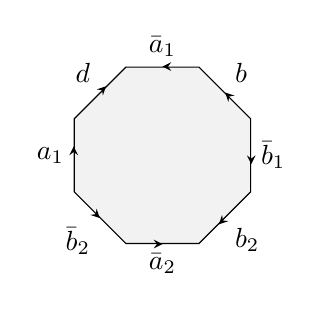
\begin{tikzpicture}


\node[fill=gray!10] (pol) [
  draw,
  minimum size=0.2\textwidth,
  regular polygon, regular polygon sides=8,
  ]{};
\foreach \x/\y/\i in {1/2/1} %\alpha's
  \path[auto=right, ->-]
    (pol.corner \x)--(pol.corner \y)
      node[midway]{$\bar{a}_1$};
\foreach \x/\y/\i in {3/4/1} %inverse \alpha's
   \path[auto=right, -<-]
     (pol.corner \x)--(pol.corner \y)
     node[midway]{$a_1$};
\foreach \x/\y/\i in {2/3/1} %\beta's
  \path[auto=right, -<-]
    (pol.corner \x)--(pol.corner \y)
      node[midway]{$d$};
\foreach \x/\y/\i in {4/5/1} %inverse \beta's
   \path[auto=right, ->-]
     (pol.corner \x)--(pol.corner \y)
     node[midway]{$\bar{b}_2$};
      \foreach \x/\y/\i in {5/6/1} %inverse \beta's
   \path[auto=right, ->-]
     (pol.corner \x)--(pol.corner \y)
     node[midway]{$\bar{a}_2$};
      \foreach \x/\y/\i in {6/7/1} %inverse \beta's
   \path[auto=right, -<-]
     (pol.corner \x)--(pol.corner \y)
     node[midway]{$b_2$};
      \foreach \x/\y/\i in {7/8/1} %inverse \beta's
   \path[auto=right, -<-]
     (pol.corner \x)--(pol.corner \y)
     node[midway]{$\bar{b}_1$};
 \foreach \x/\y/\i in {8/1/1} %inverse \beta's
   \path[auto=right, ->-]
     (pol.corner \x)--(pol.corner \y)
     node[midway]{$b$};

 
\end{tikzpicture}
\]
For example, $a_1 \sim \bar{a}_1$.  Then $$\pi_1(\Sigma_g) \cong \langle a_1, \ldots, a_g, b_1, \ldots, b_g \mid \prod_{i=1}^g [a_i, b_i] = 1 \rangle.$$ 

\begin{figure}[H]
\centering
\includegraphics[width=60mm]{M_g.png}
\caption{copied from \url{http://inspirehep.net/record/1352145/plots} \label{overflow}}
\end{figure}

We have $H_1(\Sigma_g) = \pi_1(\Sigma_g)^{\ab} = \bigoplus_{i=1}^g\left(\Z a_i \oplus \Z b_i\right)\cong \Z^{2g}.$ This induces a commutative diagram
\[
\begin{tikzcd}
\out(\pi_1(\Sigma_g)) \arrow[r, "(-)^{\ab}"] \arrow[rrd, "G"', dashed] & \aut(H_1(\Sigma_g)) \arrow[r, "\cong"] & \GL_{2g}(\Z) \arrow[d, "\det"] \\
 &  & \{\pm 1\}
\end{tikzcd}.
\]
Let $\map(\Sigma_g) =  \ker{G}$. As it turns out, $\map(\Sigma_g) \cong \faktor{\text{Diff}^+(\Sigma_g)}{\text{Diff}_0(\Sigma_g)}$, where $\text{Diff}^+$ denotes the diffeomorphisms preserving orientation and $\text{Diff}_0$ denotes the diffeomorphisms isotopic to $\id_{\Sigma_g}$.
\end{exmp}

\begin{remark}
 For the remainder of our classification problem, we assume that the subgroup of $G$ is abelian. Thus, any map $\alpha : K \to \out(H)\cong \aut(H)$ is an action.
\end{remark}

\begin{definition}
A \textit{$K$-module} is a pair $\left(A, \alpha\right)$ where $A$ is an abelian group and $\alpha : K \to \aut(A)$ is a group map.
\end{definition}

\begin{note}[Operations on $\ext(, (A, \alpha))$] $ $
\begin{enumerate}[label=(\arabic*)]
\item Let $\phi  : L \to K$ be a group map and $$1 \to A \overset{i}{\longrightarrow} G \overset{q}{\longrightarrow} K \to 1$$ be an extension. We can use $\phi$ to produce an extension of $L$ by $A$. Consider the \textit{fiber product} $G \times_K L \equiv \{(g, l) \in G \times L : q(g) = \phi(l)\}$, which is a subgroup of $G \times L$.

There is a natural map $p: G\times_K L \twoheadrightarrow L$ given by $(g, l) \mapsto l$. Also, $$\ker{p} = \left\{(g, e) : q(g) = \phi(e) =e \right\} = \left\{(g, e) : g \in A\right\} \cong A.$$ This provides us with a commutative diagram
\[ \label{eqn:fo}
\begin{tikzcd}
\quad \xi:\ 1 \arrow[r] & A \arrow[r, "i"] & G \arrow[r, "q"] & K \arrow[r] & 1 \\
\phi^{\ast}\xi :\ 1 \arrow[r] & A \arrow[r] \arrow[u, equal] & G\times_K L \arrow[r, "p"] \arrow[u] & L \arrow[u, "\phi"] \arrow[r] & 1
\end{tikzcd}. \tag{A}
\]
We call $G_{\phi^{\ast}\xi}\coloneqq  G\times_{K}L$ together with the induced map $\phi^{\ast} : G\times_{K}L\to G$ the \textit{pullback} of $q$ and $\phi$.  By construction, $\alpha^{\phi^{\ast}\xi} : L \to \aut(A)$ is given by $\alpha^{\xi} \circ \phi$. We have defined a function $\phi^{\ast} : \ext(K, (A, \alpha)) \to \ext(L, (L, \alpha \circ \phi))$. 

\item Let $A$ and $B$ be $K$ modules and $\xi$ be as in \eqref{eqn:fo}. Let $\psi: (A, \alpha) \to (B, \beta)$ be an equivariant map. We construct the \textit{pushout} $G \cup_A B$ of $i$ and $\psi$.'

Consider the action $\beta \circ q : G \to \aut(B)$. This induces a group map $i \times \psi : A \to G \ltimes_{\beta \circ q} B$ given by $a \mapsto \left(a, \psi(a)\right)$.
\begin{claim}
The map $i \times \psi$ is injective, and $$\overbrace{\im(i \times \psi)}^{A} \unlhd G \ltimes_{\beta \circ q} B.$$ Moreover, $A \leq \ker(G\ltimes_{\beta \circ q} B \twoheadrightarrow K)$.
\end{claim}
\begin{proof}
Injectivity follows from the fact that $i$ is injective. Recall that the group law on $G \ltimes_{\beta \circ q} B$ is given by $$(g_1, b_1)(g_2, b_2) = \left(g_1g_2, b_1(\beta \circ q(g_1)(b_2))\right).$$ To see that $A$ is normal, we compute
\begin{align*}
(g, b)(a, \psi(a))(g,b)^{-1} & = (g, b)(a, \psi(a) )(g^{-1}, \beta \circ q(g^{-1})(b^{-1})) 
\\ & = (ga, b\beta \circ q(g)(\psi(a)))(g^{-1}, \beta \circ q(g^{-1})(b^{-1}))
\\ &  = \left(gag^{-1}, b\beta \circ q(g)(\psi(a))\beta \circ q(ga)\beta \circ q(g^{-1})(b^{-1})\right)
\\ &  = \left(gag^{-1}, b\beta \circ q(g)(\psi(a)) \beta (q(g)\underbrace{q(a)}_{1}q(g^{-1}))(b^{-1})\right)
\\ & =  \left(gag^{-1}, b\beta \circ q(g)(\psi(a))b^{-1}\right) 
\\ & = \left(gag^{-1}, \beta \circ q(g)(\psi(a))\right)
\\ &  = \left(gag^{-1}, \psi(\alpha \circ q(g)(a))\right)
\\ &  = \left(\alpha \circ q(g)(a),  \psi(\alpha \circ q(g)(a))\right),
 \end{align*} 
which belongs to $\im(i \times \psi)$.\reversemarginpar{\marginpar{\small{Why does $\alpha \circ q(g)(a) = gag^{-1}$ hold?}}}

Finally, observe that 
\begin{align*}
\ker(G\ltimes_{\beta \circ q} B \twoheadrightarrow K) & = \left\{(g, b) : q(g) =e\right\} 
\\ & = \left\{(g, b) : g \in A\right\}
\\ &  \geq A\times \left\{e\right\} \cong A.\end{align*}
\end{proof}
Now, let $G_{\psi_{\ast}\xi}$ denote $G \cup_A B$, which equals $\faktor{G\ltimes_{\beta \circ q} B}{(i\times \psi)(A)}.$ 
We have obtained a commutative diagram.
\[ \label{eqn:cd}
\begin{tikzcd}
1 \arrow[r] & A \arrow[d, hook] \arrow[r] & G \arrow[d, hook] \arrow[r] & K \arrow[d, equal] \arrow[r] & 1 \\
1 \arrow[r] & A\times B \arrow[r, "i"] \arrow[d, two heads] & G \ltimes_{\beta \circ q} B \arrow[r, "q"] \arrow[d, two heads] & K \arrow[r] \arrow[d, equal] & 1 \\
1 \arrow[r] & \underbrace{B}_{\faktor{A\times B}{(i\times \psi)(A)}} \arrow[r] & G_{\psi_{\ast}\xi} \arrow[r] & K \arrow[r] & 1
\end{tikzcd}, \tag{B}
\]
where $B \cong \faktor{A\times B}{(i\times \psi)(A)}$ via the mapping $b \mapsto \left[(e, b)\right]$. 

Let $\psi_{\ast}$ denote the induced map $G \to G_{\psi_{\ast} \xi}$. Define the extension $\psi_{\ast}\xi$ as the bottom row of \eqref{eqn:cd}.

\item Given $\xi, \eta \in \ext(K, (A, \alpha))$, we can take $\xi \times \eta \in \ext(K \times K, (A\times A, \alpha \times \alpha))$. The diagonal map $\Delta : K \to K \times K$ is a homomorphism, as is the function $\mult: A \times A \to A$ since $A$ abelian. This is also equivariant for $\alpha \times \alpha$ and $\alpha$.
Therefore, we can form the following commutative diagram.

\[ \label{eqn:cd2}
\begin{tikzcd}
1 \arrow[r] & A\times A \arrow[r] & G_{\xi}\times G_{\eta} \arrow[r] & K\times K \arrow[r] & 1 \\
1 \arrow[r] & A\times A \arrow[r] \arrow[d, "\mult"'] \arrow[u, equal] & \left(G_{\xi} \times G_{\eta}\right) \times_{K\times K} K \arrow[r] \arrow[u] \arrow[d] & K \arrow[r] \arrow[u, "\Delta"] \arrow[d, equal] & 1 \\
1 \arrow[r] & A \arrow[r] & \left(\left(G_{\xi} \times G_{\eta}\right) \times_{K\times K} K\right) \cup_{A\times A} A \arrow[r] & K \arrow[r] & 1
\end{tikzcd} \tag{C}
\]
Define $\xi + \eta$ as the bottom row of \eqref{eqn:cd2}.
\end{enumerate}
\end{note}

\begin{exercise}
Show that $$\xi + \eta = \mult_{\ast} \Delta^{\ast}(\xi \times \eta) = \mult \circ \left(\left(\xi \times \eta\right)\circ \Delta\right) = \left(\mult \circ (\xi \times \eta)\right)\circ \Delta.$$ 
\end{exercise}

This implies that we could have taken the pushout first and then the pullback.

\begin{exercise} $ $
\begin{enumerate}
\item Verify that $\left(\ext(K, (A, \alpha)), +\right)$ is an abelian group with identity $K \ltimes_{\alpha} A$. 
\item Verify that $\phi^{\ast}$ and $\psi_{\ast}$ are homomorphisms.  
\end{enumerate}
\end{exercise}

\medskip

Suppose that $(\xi) : 1\to A \to G \to K \to 1$ is an extension. If it is not split, then by the axiom of choice there is some set-theoretic section $s: K \to G$ of $q$.
Define $f : K \times K\to G$ by $$(x, y) \mapsto s(x)s(y)s(xy)^{-1}.$$ This is a homomorphism if and only if it is constant at $e_G$. Notice that $q(f(x,y)) = e$ for any $x,y\in K$. Then $\im{f} \subset A$, giving us  $f: K\times K \to A$.
\begin{definition}
We say that $f$ is \textit{normalized} if $f(e, y) = f(x, e) =e$ for any $x,y \in K$.
\end{definition}
Note that if $s$ is \textit{normalized}, i.e., preserves the identity, then $f$ is automatically normalized.


\subsection{Lecture 16}

\begin{lemma} 
Let $\xi$ be as in \eqref{eqn:fo} with $s$ and hence $f$ normalized. Then the data $\left(K, (A, \alpha), f\right)$ determine $\xi$ up to isomorphism.
\end{lemma}
\begin{proof}
Let $G_f$ be the group with underlying set $K \times A$ and group law given by $$(x, a)(y, b) \equiv (xy, a \alpha_x(b)f(x,y)).$$ Then the diagram
\[
\begin{tikzcd}
1 \arrow[r] & A \arrow[r, "i_f"] \arrow[d] & G_f \arrow[d, "s\times i"] \arrow[r, "q_f"] & K \arrow[r] \arrow[d] & 1 \\
1 \arrow[r] & A \arrow[r, "i"] & G \arrow[r, "q"] & K \arrow[r] \arrow[l, "s", bend left] & 1
\end{tikzcd},
\]
commutes where $(s\times i)(x, a) \equiv s(x)a$.
\end{proof}

\begin{note}\label{lr}
In general, given $\left(K, \left(A, \alpha\right)\right)$ and a normalized function $f: K \times K \to A$, the formula $(x, a)(y, b) = (xy, a \alpha_x(b)f(x,y))$ defines a group law if and only if $f(x,y)f(xy, z) = \alpha_x(f(y,z))f(x, yz)$ for any $x, y, z \in K$. As $A$ is abelian, this happens if and only if  
\[ \label{eqn:star}
\alpha_x(f(y, z))f(xy, z)^{-1} f(x, yz)f(x, y)^{-1} = e. \tag{$\ast$}
\]
\end{note}

\begin{definition} $ $
\begin{enumerate}
\item We call $C^2(K, (A, \alpha))\coloneqq  \left\{f \mid f: K \times K \to A\right\}$ the set of \textit{second Hochschild cochains of $K$ with coefficients in $(A, \alpha)$}. 
\item We call $C^2(K, (A, \alpha))_0 \coloneqq  \left\{f \mid f(x, e) = f(e, y) =e\right\}$ the set of \textit{second normalized cochains}.
\item We call $Z^2(K, (A, \alpha)) \coloneqq  \left\{f \in C^2 : \eqref{eqn:star} \text{ holds}\right\}$ the set of \textit{second cocycles of $K$ with coefficients in $(A, \alpha)$}.
\end{enumerate}
\end{definition}


\Cref{lr} implies that there is a one-to-one correspondence 
\[
\left\{(\xi, s) : \xi \in \ext(K, (A, \alpha)), \ s \text{ a normalized section}\right\} \longleftrightarrow Z^2(K, (A, \alpha))_0 = Z^2 \cap C^2_0
.\]

If $\tilde{s}$ and $s$ are both normalized sections, then $c(x)\coloneqq \tilde{s}(x)s(x)^{-1}$ defines a map $c : K \to A$ such that $c(e) =e$. Let $\tilde{f}$ be the second cochain obtained from $\tilde{s}$. Then  $$\tilde{f}(x, y) = \tilde{s}(x)\tilde{s}(y)\tilde{s}(xy)^{-1} =c(x)s(x)c(y)s(y)(c(xy)s(xy))^{-1}, $$ and thus 
\begin{align*} \tilde{f}(x, y)f(x,y)^{-1} & = c(x)s(x)c(y)s(y)(c(xy)s(xy))^{-1}s(xy)s(y)^{-1}s(x)^{-1}
\\ &  = c(x)(s(x)c(y)s(x)^{-1})(s(x)s(y)s(xy)^{-1})c(xy)^{-1}s(xy)s(y)^{-1}s(x)^{-1}
\\ &  = c(x)\alpha_x(c(y))c(xy)^{-1}f(x,y)f(x,y)^{-1} 
\\ & =c(x)\alpha_x(c(y))c(xy)^{-1}.
\end{align*}
This gives us a map $\delta: C^1_0 \to Z^2_0$ defined by $c \mapsto \left((x, y) \overset{\delta_c}{\longmapsto}   c(x)\alpha_x(c(y))c(xy)^{-1}\right)$, known as the \textit{first Hochschild differential of $K$ with coefficients in $(A, \alpha)$}.  \reversemarginpar{\marginpar{\small{How do we know any first normalized cochain can be written in that form?}}}
We in turn obtain a natural map 
\[\label{eqn:HH}
\delta':\ \ext(K, (A, \alpha)) \to {HH}^2(K, (A, \alpha)) \coloneqq  \faktor{Z^2_0}{\im{\delta}}
\tag{$\star$}
\] given by $(\xi, f) \mapsto [f]$. We call ${HH}^2(K, (A, \alpha))$ the \textit{second cohomology group of $K$ with coefficients in $(A, \alpha)$}.


\begin{exercise}
Show that $\delta '$ is an isomorphism of abelian groups.
\end{exercise}

\begin{exmp}
Let us find all extensions of $\faktor{\Z}{2}\cong \M_2 \coloneqq  \{\pm1\}$ by $\Z$, i.e., classify all short exact sequences of the form
\[
\begin{tikzcd}
1 \arrow[r] & \Z \arrow[r] & G \arrow[r] & \M_2 \arrow[r] & 1
\end{tikzcd}
\]
\underline{Case 1:} $\M_2$ acts trivially on $\Z$. 

Then $C^2_0 = \left\{f : \M_2 \times \M_2 \to \Z \mid f(1, y) = f(x, 1) = 0 \text{ for any } x,y \in \M_2 \right\}$. Each $f \in C^2_0$ is thus determined by $f(-1, -1)$, so that $C^2_0 \cong \Z$ via $f\mapsto f(-1, 1)$.

\medskip

 Note that $f\in Z^2_0 \iff f(y, z)-f(xy, z)+f(x, yz)-f(x, y) =0$ for any $x, y, z\in \M_2$. It's easy to check this is always satisfied. Hence $Z^2_0 \cong \Z$ as well. 

\medskip

 Moreover, $C^1_0 = \{c : \M_2 \to \Z : c(1) =0\} \cong \Z$, yielding the correspondence $$\Z \ni b \longleftrightarrow \left(c: {-1} \mapsto b\right).$$ Then the differential $\delta : C^1_0 \to Z^2_0\cong \Z$ is given by $\delta_c(x, y) = c(x)+c(y) -c(xy)$, so that $\delta_c({-1}, {-1}) = c({-1}) + c({-1}) = 2b$. That is, $\delta : \Z \to \Z$ is given by $b \mapsto 2b$. This implies that ${HH}^2 = \faktor{\Z}{2}$, so that the only nontrivial extension is precisely
\[
\begin{tikzcd}
1 \arrow[r] & \Z \arrow[r, "\mult_2"] & \Z \arrow[r] & \faktor{Z}{2} \arrow[r] & 1
\end{tikzcd}.
\]
\underline{Case 2:} The action is nontrivial with ${-1} \mapsto \left(n \mapsto {-n}\right)$. 

 Again, we get $C^2_0 \cong \Z$. Moreover, if $f\in Z_2^0$ and $y= z = {-1}$, then 
\begin{align*}
0 & = \alpha_x(f({-1}, {-1})) - f({-x}, {-1})+ f(x, 1)- f(x, {-1})
\\ & = \alpha_x(\underbrace{f({-1}, {-1})}_a) - f({-x}, {-1})- f(x, {-1}) 
\\ & =
\begin{cases}
0 & x =1 \\
{-2a} & x = {-1}
\end{cases}.
\end{align*}
Hence $a = 0$, and $f = 0$. This implies that ${HH}^2 = 0$ with $\Z \rtimes_{\alpha} \M_2$ being the unique extension. 
\end{exmp}

\section{Categories and functors}

\subsection{Lecture 17}

\begin{definition} 
A \textit{category $\c$} consists of
\begin{itemize}
\item a class of \textit{objects $\ob{\c}$},
\item a class of \textit{morphisms $\mor{\c}$},
\item a set $\Hom_{\c}(x,y)$ of morphisms with \textit{source} $x$ and \textit{target} $y$ for each $x,y \in \ob{\c}$, and
\item a partial  \textit{composition} function $\circ : \Hom_{\c}(x,y) \times \Hom_{\c}(y,z) \to \Hom_{\c}(x,z)$ where $(f,g) \mapsto g \circ f$.
\end{itemize}
These data must satisfy the following properties.
\begin{enumerate}[label=(\roman*)]
\item $\mor{\c} = \coprod_{x,y\in \ob{\c}} \Hom_{\c}(x,y)$.
\item Composition is associative.
\item For each $x\in \ob{\c}$, there is an \textit{identity morphism $\id_x: x \to x$} such that $f \circ \id_x = f$ and $\id_x \circ g = g$ for any maps $f: x \to y$ and $g: z \to x$.
\end{enumerate}
\end{definition}

\smallskip

When $\c$ is small, we see that $\left(\mor{\c}, \circ\right)$ is a partially defined monoid encoding all information about $\c$. We may believe, therefore, that monoid homomorphisms are the correct tools for comparing categories. These, however, are not flexible enough. In particular, an isomorphism of monoids will prove stronger than our chosen notion of equivalence of categories.

\smallskip

\begin{exmp} The following are examples of categories.
\begin{enumerate}
\item $\mathbf{Set}$, the category of all sets with functions as morphisms.
\item $\mathbf{Grp}$, the category of all groups with group homomorphisms as morphisms.
\item $\mathbf{Ab}$, the category of all abelian groups.
\item $\mathbf{Top}$, the category of all topological spaces with continuous maps as morphisms.
\item $C^k{-}\mathbf{Mfld}$, the category of all $C^k$-manifolds with $C^k$ maps as morphisms.
\item $\mathbf{Vect}_k$, the category of all vector spaces over a field $k$ with linear maps as morphisms.
\item The \textit{simplicial category $\varDelta$} has all finite ordinals $\left[n\right] \coloneqq \left\{0 < 1 < \cdots < n\right\}$ as objects and all functions $f : \left[m\right] \to \left[n\right]$ satisfying $a \leq b \implies f(a) \leq f(b)$ as morphisms.
\item Recall the functor category $\mathbf{sSet} \coloneqq \Fun(\varDelta^{\op}, \mathbf{Set})$ of simplicial sets (cf. \cref{funct} below). We can view simplicial sets as books that record the combinatorics of gluing
simplices into a topological space. 

 Also, recall the \textit{standard $n$-simplex} $$\Delta^n = \left\{(t_0, \ldots, t_n) \in \R^{n+1} : t_i \geq 0, \ \sum_{i=0}^n t_i =1\right\}.$$ In this case, we send a morphism $f : [m] \to [n]$ to the map $$\Delta_f : \R^{m+1} \to \R^{n+1}, \ \quad e_i \mapsto e_{f(i)},$$ which is linear over $\R$. We see that $\Delta_f(\Delta^m) \subset \Delta^n$, where $\Delta_f(\Delta^m)$ is either a face of $\Delta^n$ or the entire simplex $\Delta^n$. Note that $\Delta^{(-)}$ is a covariant functor $\varDelta \to \mathbf{Set}$, hence a \textit{cosimplicial set}. 


Given a simplicial set $X_{\bullet}$, endow each set $X_n$ with the discrete topology. Define the \textit{geometric realization of $X_{\bullet}$} as the space $$\left\lvert{X_{\bullet}}\right\rvert \equiv \faktor{\coprod_{m\geq 0}{\left(X_m \times \Delta^m\right)}}{\sim}$$ where $X_n \times \Delta^n \ni \left(x, y\right)\sim \left(x', y'\right) \in X_m \times \Delta^m$ if $X(f)(y') = y$ and $\Delta_f(x) = x'$ for some morphism $f: [n] \to [m]$.  
\item  We have the category of  \textit{correspondences} $\mathbf{Corr}$ with objects all sets and morphisms all binary relations. Given any two binary relations $u\subset X\times Y$ and $v \subset Y \times Z$, let
 $$v \circ u = \left\{(x, y) \in X \times Z : \left(\exists b \in Y\right)\left((x, b) \in u \text{ and }(b, y) \in v\right)\right\}.$$ Then the identity morphisms are precisely the diagonal maps.
\item Let $\left(I, \leq \right)$ be a partially ordered set. Then we have the \textit{order category $I$ associated to $\leq$} with $\ob(I) \equiv I$ and for any $x,y\in I$,
\[
\Hom_I(x,y) \equiv 
\begin{cases} 
\left\{x\overset{i}{\rightarrow} y\right\} & x\leq y
\\ \emptyset & \text{otherwise}
\end{cases}.
\]
\item Let $\mathbf{Ouv}_X$ denote the category of open sets of a topological space $\left(X, \tau\right)$ with inclusion maps as morphisms.
 This is precisely the order category of $\tau$ associated to the poset $\subseteq$. 
 \item For any category $\c$, we have the \textit{opposite category $\c^{\op}$} where $\ob{\c^{\op}} \equiv \ob{\c}$ and $\Hom_{\c^{\op}}(x,y) \equiv \Hom_{\c}(y,x)$. Thus, $\c^{\op}$ is formed by keeping the objects but switching all of the arrows in $\c$.
\item Let $G$ be a group. Then the \textit{classifying category $B{G}$ of $G$} is the category with a single object $\ast$ and $\Hom_{B{G}}(\ast, \ast) \equiv G$. Composition here is given by the group law of $G$, and the identity morphism is precisely $e_G$. 

Note that $B\left(G^{\op}\right) =\left(BG\right)^{\op}$.

\begin{aside}
Suppose that $G$ is a discrete group. Then the geometric realization $\left\lvert{N(B{G})}\right\rvert$ of the nerve  of $B{G}$ is homotopy equivalent to the classifying space for principal $G$-bundles.
\end{aside}
\end{enumerate}
\end{exmp}

\begin{definition}\label{funct}
Let $\c$ and $\d$ be categories. A \textit{(covariant) functor $F: \c \to \d$ from $\c$ to $\d$} consists of two functions $F: \ob{\c} \to \ob{\d}$ and $F: \mor{\c} \to \mor{\d}$ such that 
\begin{enumerate}[label=(\roman*)]
\item $F(f) : F(x) \to F(y)$ in $\d$ whenever $f: x \to y$ in $\c$,
\item $F(f \circ g) = F(f) \circ F(g)$, and 
\item $F(\id_x) = \id_{F(x)}$.
\end{enumerate}
\end{definition}

\begin{term} $ $
\begin{enumerate}
\item We call  a covariant functor  $\c^{\op} \to \d$ a \textit{contravariant} functor $\c \to \d$.
\item We call a contravariant functor $\c \to \d$ a \textit{presheaf of $\c$ with values in $\d$}.
\end{enumerate}
\end{term}

\smallskip

We now can form the category $\mathbf{Cat}$ of all small categories with functors between them as morphisms.

\subsection{Lecture 18}

\begin{exmp}  The following are examples of functors.
\begin{enumerate}
\item We have a family of \textit{forgetful} functors $U : \c \to \d$, which simply forget certain structure which the objects in $\c$ carry.
\begin{gather*}
\mathbf{Grp} \to \mathbf{Set}
\\ \mathbf{Ab} \to \mathbf{Set}
\\ \mathbf{Vect}_k \to \mathbf{Ab}
\\ \mathbf{Vect}_k \to \mathbf{Set}
\end{gather*} 

Let $\mathbf{Ring}$ denote the category of (unital) rings. Then the forgetful functor $\G_A: \mathbf{Ring} \to \mathbf{Ab}$ is known as the \textit{additive group functor}.
\item Let $f: X \to Y$ be a map of spaces. Define the \textit{section functor}
 \begin{gather*}
 \Gamma_f: \mathbf{Ouv}_Y^{\op} \to \mathbf{Set}
 \\
\mho \mapsto \left\{\underset{\text{continuous}}{s: \mho \to X} \mid f \circ s = \id_{\mho}\right\}
\\ \Gamma_f(\mho \subset V) : \left(s: V \to X\right) \mapsto \left(s\restriction_{\mho} : \mho \to X\right).
\end{gather*} This is also denoted by $\Gamma_{\faktor{X}{Y}}$.
\item Let $n\geq 0$ be an integer. We have the \textit{homology functor} $H_n(-, \Z) : \mathbf{Top} \to \mathbf{Ab}$ sending each space $X$ to $H_n(X, \Z)$, the \textit{$n$-th singular homology of $X$}.
\item For each $n\geq 1$, the general linear group functor $\GL_n(-) : \mathbf{CommRing} \to \mathbf{Grp}$, defined on morphisms by sending a ring map $f: R \to S$ to the group map $\GL_n(R) \to \GL_n(S)$ given by sending a matrix $M$ over $R$ to the matrix $f(M)$ over $S$ obtained by applying $f$ to each entry of $M$.
\item The homotopy functor $\pi_i : \mathbf{Top_{\ast}^{\text{(conn, lc)}}} \to
 \begin{cases} 
\mathbf{Set} & i=0
\\ \mathbf{Grp} & i = 1 \\
\mathbf{Ab} & i >1
\end{cases}.$
\item Define the functor  $(-)_{\bullet} : \mathbf{Set} \to {\mathbf{sSet}}$ by sending each set $S$ to the \textit{constant/discrete} functor $(S)_{\bullet}$ at $S$, i.e.,  $S_n \equiv S$ for every $n\geq 0$.

Alternatively, say that an $n$-simplex  $x\in X_n$ is \textit{nondegenerate} if it is \emph{not} of the form $x =s_i(y)$ where $1\leq i \leq n-1$ and $y\in X_{n-1}$ and let $X_n^{\nd}$ denote the subset of all nondegenerate $n$-simplices.  Define $(S)_{\bullet}$ as the unique simplicial set such that $$S_n^{\nd} = \begin{cases}
S & n =0 \\ \emptyset & n > 0 \end{cases}.$$ Then
 $\left\lvert{(S)_{\bullet}}\right\rvert$ is homotopy equivalent to $S$ equipped with the discrete topology. 
\item The geometric realization functor $\left\lvert{\cdot}\right\rvert : \mathbf{sSet} \to \mathbf{Top}$.
\item Define the \textit{singular chains functor $\Sing_{\bullet} : \mathbf{Top} \to \mathbf{sSet}$} by
\begin{gather*}
 \Sing_n(X) \equiv \left\{\phi \mid \underset{\text{continuous}}{\phi  : \Delta^n \to X}\right\} \quad \ \quad \left(f: [m] \to [n]\right) \mapsto \left(\Sing_f(X) : \phi \mapsto \phi \circ \Delta_f\right)
 \\ \Sing_n(u : X \to Y) : \Sing_n(X) \to \Sing_n(Y),\ \quad \phi \mapsto u \circ \phi.
 \end{gather*}
\begin{aside} This is right adjoint to the geometric realization functor. \end{aside}
\item If $n=1,2$, then we have the functor ${HH}^n(G, -) : {}_{G}\mathbf{Mod} \to \mathbf{Ab}$ as in \eqref{eqn:HH}. This extends to all $n\in \Z_{\geq 1}$.
\end{enumerate}
\end{exmp}

\smallskip

\begin{definition}
Let $F$ and $G$ be functors $\c \to \d$. A \textit{natural transformation $\phi: F\Rightarrow G$ from $F$ to $G$} is a class function $\phi_{(-)}: \ob{\c} \to \mor{\d}$ such that $\phi_x$ is a morphism $F(x) \to G(x)$ and for each morphism $h: x\to y$ in $\c$, the square
\[
\begin{tikzcd}
F(x) \arrow[d, "\phi_x"'] \arrow[r, "F(h)"] & F(y) \arrow[d, "\phi_y"] \\
G(x) \arrow[r, "G(h)"']                  & G(y)                 
\end{tikzcd}
\] commutes. The maps $\left(\phi_x\right)_{x\in \ob{\x}}$ are called the \textit{components of $\phi$}.
\end{definition}

When $\c$ is small, this gives us the \textit{functor category $\mathbf{Fun}(\c, \d)$} consisting of all functors $\c \to \d$ with natural transformations between them as morphisms. Here, composition is given componentwise by $\left(A \circ B\right)_x \equiv A_x\circ B_x$, and the identity map is given componentwise by $\left(\id_F\right)_x \equiv \id_{F(x)}$.

\smallskip

\begin{definition}
A morphism $\phi : A \to B$ in $\c$ is an \textit{isomorphism} if $\psi \circ \phi = \id_A$ and $\phi \circ \psi = \id_B$ for some morphism $\psi : B \to A$ in $\c$. In this case, we write $A\cong B$.
\end{definition}

\begin{term}
An isomorphism in a functor category is called a \textit{natural isomorphism}.
\end{term}

\begin{exercise}
Show that a natural transformation is an isomorphism if and only if each component is an isomorphism.
\end{exercise}

\smallskip

\begin{exmp} The following are examples of natural transformations.
\begin{enumerate}
\item The determinant $\det : \GL_n(\mathbb{F}) \to \GL_1(\mathbb{F})$.
\item The \textit{Hurewicz map} $\hur: \pi_1 \to H_1$.  The universal property of $(-)^{\ab}$ induces a commutative diagram of functors
\[
\begin{tikzcd}
\pi_1 \arrow[r, "\hur"] \arrow[d, "(-)^{\ab}"'] & H_1 \\
(\pi_1)^{\ab} \arrow[ru, "q"', dashed] & 
\end{tikzcd}
.\] Hurewicz's theorem states that $q$ is actually an isomorphism in $\mathbf{Fun}(\left(\pi_1\right)^{\ab}, H_1)$.
\end{enumerate}
\end{exmp}

\smallskip

\begin{exmp}
Consider the \textit{dualization functor} $(-)^{\vee} : \mathbf{Vect}_k^{\op}  \to \mathbf{Vect}_k$ given by
\begin{gather*}
V \mapsto V^{\vee} \equiv \Hom(V, k)
\\ \left(f: V \to W\right) \mapsto \left( \phi \mapsto \phi \circ f\right).
\end{gather*}  
There is an analogous functor $(-)^{\vee} : \mathbf{Vect}_k \to \mathbf{Vect}_k^{\op}$. The \textit{double dualization} functor $(-)^{\ast \ast}: \mathbf{Vect}_k \to \mathbf{Vect}_k$ is the composite of these, inducing a map of functors $\epsilon: \id_{\mathbf{Vect}_k} \to (-)^{\vee \vee}$ given componentwise by $$\epsilon_V : x \mapsto \left(\phi \mapsto \phi(x)\right).$$
\end{exmp}

\begin{exercise}  $ $
\begin{enumerate} 
\item Show that $\epsilon$ is not a natural isomorphism by showing that if $V$ is an infinite-dimensional $\R$-space with a countable basis, then $V^{\ast}$ and hence $V^{\vee \vee}$ have uncountable bases.
\item Show, however, that it is an isomorphism in the setting of finite-dimensional vector spaces over $k$.
\end{enumerate}
\end{exercise}

\begin{definition} $ $
\begin{enumerate}
\item We say that a category $\c$ is \textit{small} if $\ob{\c}$ is a set.
\item Let $\pi_0(\c)$ denote the class of equivalence classes $\faktor{\ob \c}{\cong}$. We say that $\c$ is \textit{essentially small} if $\pi_0(\c)$ is a set.
\end{enumerate}
\end{definition}

\subsection{Lectures 19 and 20}

We want a weaker notion of sameness between categories that \textit{isomorphism}.

\begin{definition}
A functor $F: \c \to \d$ is an \textit{equivalence} if there is a functor $G: \d \to \c$ such that $F \circ G \cong \id_{\d}$ and $G\circ F \cong \id_{\c}$. In this case, we say that $G$ is a \textit{quasi-inverse of $F$} and that $\c$ and $\d$ are \textit{equivalent}.
\end{definition}

This is weaker than \textit{isomorphism} as $F\circ G$ and $G\circ F$ need not be \textit{equal} the identity functor.

\smallskip

\begin{exmp}\cref{vect}
Let $\c = \mathbf{Vect}_k^n$, which consists of all $n$-dimensional vector spaces over $k$, and $\d =  B{\Mat_n(k)}$. Consider the functor $F : \d \to \c$ defined on objects by $\ast \mapsto k^n$ and on morphisms by $A \mapsto \left(v \mapsto Av\right)$. Define the functor $G: \c \to \d$ using the axiom of choice as follows. Choose a basis for each space $V \in \c$ and send each linear map $f$ to the matrix of $f$ with respect to the two chosen bases. Then $F$ is an equivalence with quasi-inverse $G$.
\end{exmp}

\smallskip

\begin{exercise}
Show that $\c$ is essentially small  if and only if it is equivalent to a small category. 
\end{exercise}

\medskip

Any functor $F: \c \to \d$ induces a map $\pi_0(F) : \pi_0(\c) \to \pi_0(\d)$ because $F$ maps isomorphisms to isomorphisms. If $F$ is an equivalence with quasi-inverse $G$, then this is a bijection with $\pi_0(G)$ as inverse. Therefore, any two equivalent categories have the same collection of isomorphism classes of objects.


\begin{definition}
We say that $F$ is \textit{essentially surjective} if $\pi_0(F)$ is surjective. 
\end{definition}

\smallskip

\begin{definition}
If $\c$ is a category, then a category $\a$ is a \textit{subcategory of $\c$} if
\begin{enumerate}[label=(\roman*)]
\item $\ob{\a}$ is a subclass of $\ob{\c}$, 
\item $\Hom_{\a}(x,y) \subset \Hom_{\c}(x,y)$ for any $x,y\in \ob{\a}$, and
\item composition and identity in $\a$ are exactly as they are in $\c$.
\end{enumerate}
\end{definition}

\smallskip

Any subcategory $\a$ of $\c$ yields an inclusion functor $i : \a \to \c$.  \Cref{vect} shows that the inclusion functor $B{\Mat_n(k)} \to \mathbf{Vect}_k^n$ is an equivalence. 

\medskip

\begin{definition} Let $F: \c \to \d$ be a functor. Consider the set map $F({-}): \Hom_{\c}(x,y) \to \Hom_{\d}(F(x), F(y))$.
\begin{enumerate}
\item We say that $F$ is \textit{faithful} if $F({-})$ is injective.
\item We say that $F$ is \textit{full} if $F({-})$ is surjective. 
\item We say that $F$ is \textit{fully faithful} if it is both full and faithful, i.e., $F({-})$ is bijective.
\end{enumerate}
\end{definition}

\begin{exmp}
The inclusion functor $i : \a \to \c$ is faithful.
\end{exmp}

\smallskip


\begin{exercise}
Show that a functor is an equivalence if and only if it is fully faithful and essentially surjective.
\end{exercise}



\section{The Yoneda lemma}

Notice that $\Hom_{\mathbf{Set}}(\ast, x) \cong x$ for any set $x$ via the mapping $f \mapsto f(\ast)$. In a general category $\c$, we may not have an initial object $\ast$, like a singleton. In order to view objects in $\c$ as themselves collections of objects, we define the following notion.

\begin{definition}
Given $x \in \ob \c$, a \textit{$y$-point/probe of $x$} is the set $\Hom_{\c}(y, x)$.
\end{definition}
The class $\left\{\Hom_{\c}(y, x)\right\}_{y\in \ob \c}$ of $y$-points reconstructs $x$ as an object in $\c$. To see this, consder the presheaf category $$\widehat{\c}\coloneqq  \Fun(\c^{\op}, \mathbf{Set})$$ and let $x \in \ob \c$. Define the functor $h_x : \c^{\op} \to \mathbf{Set}$ on objects and morphisms, respectively, by 
\begin{gather*}
y \mapsto \Hom_{\c}(y, x)
\\ h_x(f) : u \mapsto u \circ f.
\end{gather*}

\begin{definition}
A presheaf $F \in \widehat{\c}$ is \textit{representable} if $F \cong h_x$ for some $x\in \ob{\c}$. We say that \textit{$x$ represents $F$} in this case.
\end{definition}
The assignment $h: \c \to \widehat{\c}$ given by $x \mapsto h_x$ is a functor where $h(\phi : x \to x')$ is given by $$h(\phi)_y : \Hom_{\c}(y, x) \to \Hom_{\c}(y, x'),\ \quad u \mapsto \phi \circ u.$$ This is called the \textit{Yoneda functor}. The essential image of $h$ consists of all representable presheaves of $\c$.


\begin{lemma}[Yoneda] Let $\c$ be a category.
\begin{enumerate}[label=(\arabic*)]
\item For any $x, y \in \ob \c$, the map $\Hom_{\c}(x, y) \to \Hom_{\widehat{\c}}(h_x, h_y)$ given by $\phi \mapsto h(\phi)$ is bijective, i.e., $h : \c \to \widehat{\c}$ is fully faithful.
\item There is a natural isomorphism $$\Hom_{\c}(-, -) \cong \Hom_{\widehat{\c}}\left(h_{(-)}, h_{(-)}\right)$$ of functors $ \c^{\op} \times \c \to \mathbf{Set}$.
\end{enumerate}
\end{lemma}
Thanks to (2), we can treat objects in $\c$ as set-valued presheaves of $\c$.
\begin{proof}
We prove just the first statement, from which the second follows formally.
Let us define an inverse $i:  \Hom_{\widehat{\c}}(h_x, h_y) \to \Hom_{\c}(x, y)$ of the given map. If $\alpha : h_x \to h_y$ is a morphism in $\widehat{\c}$, then let $$i(\alpha) = \alpha_x(\id_x).$$ Note that $\alpha_x(\id_x) \in h_y(x) = \Hom_{\c}(x,y)$.

\medskip

 If $f: x \to y$ in $\c$, then $h(f)$ is a map $h_x \to h_y$ and $h(f)_z : \Hom_{\widehat{\c}}(z, x) \to \Hom_{\widehat{\c}}(z, y)$ is given by $(-) \mapsto f \circ (-)$ for any $z\in \ob \c$. In this case, $h(f)_x(\id_x) = f\circ \id_x = f$. This proves that $i$ is a left inverse of $h$.

\medskip

 It remains to show that $i$ is a right inverse of $h$. Let $\alpha$ be a map $h_x \to h_y$.  We have that $
i(\alpha) = \alpha_x(\id_x) \in h_y(x)$, so that $i(\alpha)$ is a morphism $x \to y$ in $\c$. Note that the component map $h(i(\alpha))_z : \Hom_{\c}(z, x) \to \Hom_{\c}(z, y)$ is given by $\phi \mapsto i(\alpha) \circ \phi.$ We must check that this agrees with $\alpha_z$. For any $z \in \ob \c$ and map $\phi : z \to x$ in $\c$, the square
\[
\begin{tikzcd}
h_x(x) \arrow[r, "\alpha_x"] \arrow[d, "h_x(\phi)"'] & h_y(x) \arrow[d, "h_y(\phi)"] \\
h_x(z) \arrow[r, "\alpha_z"'] & h_y(z)
\end{tikzcd}
\] commutes
because $\alpha$ is a natural transformation. By evaluating this at the morphism $\id_x$, we see that 
\[
\left(\alpha_{z} \circ h_{x}(\phi)\right)\left(\mathrm{id}_{x}\right)=\left(h_{y}(\phi) \circ \alpha_{x}\right)\left(\mathrm{id}_{x}\right)
.\] But the lefthand side equals $\alpha_{z}\left(h_{x}(\phi)\left(\mathrm{id}_{x}\right)\right)=\alpha_{z}\left(\mathrm{id}_{x} \circ \phi\right) = \alpha_z(\phi)$, and the righthand side equals $h_y(\phi)(i(\alpha)) = i(\alpha) \circ \phi$.
That is, $\alpha_z(\phi) = i(\alpha) \circ \phi$, as required.
\end{proof}

Let $F \in \widehat{\c}$. Recall that $F$ is representable by $x$ if there is some isomorphism of functors $h_x \cong F$. By our proof of the Yoneda lemma, this is completely determined by the object $\xi\coloneqq  h_x(\id_x) \in F(x)$. Conversely, given $\xi \in F(x)$, we get a natural map \begin{align*}
h_x(y) &  \to F(y)
\\  f &  \mapsto F(f)(\xi).
\end{align*} This defines a map of functors $\eta^{\xi} : h_x \to F$ where $\eta^{\xi}_y(f) = F(f)(\xi)$ for every $y \in \ob \c$. 

\medskip

 By the Yoneda lemma, $F$ is representable by $x$  if and only if there is some $\xi \in F(x)$ such that $\eta^{\xi}$ is an isomorphism. 

\begin{exmp} $ $
\begin{enumerate}
\item Define the presheaf $\P : \mathbf{Set}^{\op} \to \mathbf{Set}$ on objects by $S \mapsto \P(S)$ and on morphisms by $\P(f : S \to T) : A \mapsto f^{-1}(A).$ For $\P$ to be representable, we need to find some set $Q$ and $\xi \subset Q$ such that $\Hom(S, Q) \to \P(S)$ given by $u \mapsto u^{-1}(\xi)$ is a bijection for every set $S$. We can do so by setting $Q = \{0, 1\}$ and $\xi = \{1\}$ since $\Hom(S, \{0, 1\}) \cong \P(S)$ via the characteristic function on $S$.
\item Consider the forgetful presheaf $U: \mathbf{Ring} \to \mathbf{Set}$ on  $\mathbf{Ring}^{\op}$.  For any unital ring $R$, any ring map $\phi : \Z[t] \to R$ is determined by the value $\phi(t)$. Therefore, the map $\Hom_{\mathbf{Ring}}( \rho, R) \to R$ given by $u \mapsto U(u)(\xi)$ is bijective where $\rho \equiv \Z[t]$ and $\xi \equiv t$ (which belongs to $U(\Z[t])$). This shows that $U$ is represented by $\Z[t]$.
\end{enumerate}
\end{exmp}

\begin{exmp}[Tensor product]
Let $V, W \in \ob \mathbf{Vect}_k$ and define the presheaf $B: \mathbf{Vect}_k \to \mathbf{Set}$ on $\left( \mathbf{Vect}_k\right)^{\op}$ by $$L \mapsto \left\{ \phi : V \times W \to L \mid \phi \text{ bilinear}\right\}.$$ We want to find some $k$-vector space $T$ and some bilinear map $\xi \in B(T)$ such that the map $\Hom_{\left( \mathbf{Vect}_k\right)^{\op}}(L, T) \to B(L)$ given by $u \mapsto u \circ \xi$ is bijective for any space $L$. 
\[
\begin{tikzcd}
V \times W \arrow[r, "\xi"] \arrow[rd] & T \arrow[d, "u"] \\
 & L
\end{tikzcd}
\]
We construct such a pair $(T, \xi)$ as follows. Let $\mathcal{F}$ denote the vector space of set maps $f: V \times W \to k$ such that $\supp(f)$ is finite. A basis for $\mathcal{F}$ is given by the delta functions of points $(x, y) \in V \times W$, defined by
\[ \delta_{(x,y)}(a, b) = \begin{cases}
0 & (a,b) \ne (x,y) \\
1 & (a, b) = (x,y)
\end{cases}
\]
Now, let $\mathcal{F}_0 \subset \mathcal{F}$ be the subspace spanned by elements of any of the forms
\begin{gather*}
 \delta_{(x' + x'', y)} - \delta_{(x', y)} - \delta_{(x'', y)} 
 \\ \delta_{(x, y' + y'')} - \delta_{(x, y')} - \delta_{(x, y'')} 
\\ \delta_{(cx, y)} - c\delta_{(x,y)}  
\\\delta_{(x,cy)} -c \delta_{(x,y)} 
\end{gather*}
where $x, x', x'' \in V$ and $y, y', y'' \in W$ and $c \in k$. Finally, set $T = \faktor{\mathcal{F}}{\mathcal{F}_0}$ and define $\xi$ by  $(x, y) \mapsto \delta_{(x,y)} + \mathcal{F}_0$. Then $T$ represents $B$. We usually write $V \otimes_k W$ for $T$.
\end{exmp}

\bigskip

 Instead of constructing the real numbers as equivalence classes of Cauchy sequences or as Dedekind cuts, we want to find a special property distinguishing $\R$ (equivalently, an open or closed interval) in  $\mathbf{Top}$. 

We can pick out the interval $[0,1]$ among all topological spaces as follows. We see that $$[0,1]\cong \left( \faktor{[0,1] \coprod [0,1]}{\text{first 1 = second 0}} \right)$$ via the mean function $M$. Let $\c$ denote the category of pairs $(X, \alpha)$ where $X$ is a topological space with two ordered marked points $\ell_x$ and $r_x$  along with a map $\alpha :  \faktor{X \coprod X}{\sim} \overset{\cong}{\longrightarrow} X$ where the first $r_x$ is equal under $\sim$ to the second $\ell_x$.
 
\begin{theorem}[Freyd]
$\left([0,1], M\right)$ is the terminal object in $\c$.
\end{theorem}

\subsection{Lecture 21}

\begin{definition} Let $\c$ be a category and $I$ be any set. Suppose that $A_{\alpha} \in \ob \c$ for each $\alpha \in I$.
\begin{enumerate}
\item  Define the \textit{product functor} $\c^{\op} \to \mathbf{Set}$ by $$B \mapsto \prod_{\alpha \in I}\Hom_{\c}(B, A_{\alpha}), \  \quad f \mapsto \left(f_{\alpha} \mapsto f_{\alpha} \circ f\right).$$ If the product functor is representable by some object $P$ in $\c$, then we say that $P$ is the \textit{product} of the $A_{\alpha}$ in $\c$. (This wording makes sense as limits are unique up to isomorphism.)
\item Define the \textit{coproduct functor} $\c \to \mathbf{Set}$ by $$ B \mapsto \prod_{\alpha \in I} \Hom_{\c}(A_{\alpha}, B), \  \quad f \mapsto \left(f_{\alpha} \mapsto f \circ f_{\alpha}\right).$$ If the coproduct functor is representable by some object $Q$ in $\c$, then we say that $Q$ is the \textit{coproduct} of the $A_{\alpha}$ in $\c$.
\end{enumerate}
\end{definition}

 By the Yoneda lemma, if $P$ is the product of $\left\{A_{\alpha}\right\}$, then there is some $\xi \coloneqq \left\{\pr_{\alpha} : P \to A_{\alpha}\right\}_{\alpha} \in \prod_{\alpha}\Hom_{\c}(P, A_{\alpha})$ such that $$\eta^{\xi}_B : h_P = \Hom_{\c}(B, P) \to \prod_{\alpha}\Hom_{\c} (B, A_{\alpha}), \  \quad f \mapsto \left\{\pr_{\alpha} \circ f\right\}_{\alpha}$$ is a natural bijection in $B \in \ob \c$. This gives an isomorphism of set-valued presheaves $h_P \cong \Hom_{\c}(-, A_{\alpha})$. Let $$\prod_{\alpha} A_{\alpha} \coloneqq  P.$$ Then we have a natural bijection $\Hom_{\c}(B, \prod_{\alpha} A_{\alpha}) \cong \prod_{\alpha} \Hom_{\c}(B, A_{\alpha})$ in $B$.

 Likewise, if $Q$ is the coproduct of $\left\{A_{\alpha}\right\}$, then by viewing the coproduct functor as a presheaf on $\c^{\op}$ we get some $\xi\coloneqq  \left\{i_{\alpha} : A_{\alpha} \to Q\right\}_{\alpha} \in \prod_{\alpha}\Hom_{\c}(A_{\alpha}, Q)$ such that $$\Hom_{\c} (Q, B) \overset{\cong}{\longrightarrow} \prod_{\alpha}\Hom_{\c}(A_{\alpha}, B), \ \quad f \mapsto \left\{f \circ i_{\alpha}\right\}_{\alpha}$$ for each $B\in \ob \c$. Let $$\coprod_{\alpha} A_{\alpha} \coloneqq  Q.$$ Then $\Hom_{\c}\left(\coprod_{\alpha} A_{\alpha}, B\right) \cong \prod_{\alpha}\Hom_{\c}(A_{\alpha}, B)$ for each $B$.
 
 \begin{notation}
 The symbol $\bigoplus$ may be used in place of $\coprod$.
 \end{notation}


\begin{exmp} $ $
\begin{enumerate}
\item $\mathbf{Set}$ has all products and coproducts, in the form of Cartesian products and disjoints unions, respectively.
\item Let $R$ be a unital ring and $\c = \mathbf{Mod}_R$, the category of $R$-modules, i.e., pairs $(M, \rho)$ where $M$ is an abelian group and $\rho$ is a map $R \to \ed(M)$ satisfying 
\begin{align*}  \rho(0) &= 0  \\  \rho(1_R) &= \id_M \\   \rho(a +b) &= \rho(a) + \rho(b)  \\  \rho(ab) &= \rho(a) \circ \rho(b). \end{align*} The morphisms $(M, \rho) \to (N, \lambda)$ are precisely the group homomorphisms $\phi : M \to N$ intertwining $\rho$ and $\lambda$, i.e., for any $x \in R$, the square
\[
\begin{tikzcd}
M \arrow[d, "\phi"'] \arrow[r, "\rho(x)"] & M \arrow[d, "\phi"] \\
N \arrow[r, "\lambda(x)"] & N
\end{tikzcd}
\] commutes.

Let $\left\{\left(A_{\alpha}, \rho_{\alpha}\right)\right\}_{\alpha \in I}$ be a collection of $R$-modules. If we endow the Cartesian product $\prod_{\alpha} A_{\alpha}$ with the componentwise module structure inherited from the $A_{\alpha}$, then it becomes the product of $\left\{A_{\alpha}\right\}$ in $\mathbf{Mod}_R$. Specifically, the underlying group law and zero element are given by 
\begin{align*}
\left(a_{\alpha}\right)_{\alpha \in I} + \left(b_{\alpha}\right)_{\alpha \in I} & \equiv \left(a_{\alpha} + b_{\alpha}\right)_{\alpha \in I}
\\  0&  \equiv \left(0\right)_{\alpha \in I}
,\end{align*} and scalar multiplication is given by
\[
\left(\prod_{\alpha} \rho_{\alpha}\right)(x)\left(\left(a_{\alpha}\right)\right)=\left(\rho_{\alpha}(x)\left(a_{\alpha}\right)\right), \quad x\in R
.\] 

Moreover, the coproduct (or direct sum) of $\left\{A_{\alpha}\right\}$ is defined as the submodule of the product consisting of all tuples $(a_{\alpha})$ such that $a_{\alpha} \ne 0$ for at most finitely many $\alpha \in I$. This means that the product and coproduct coincide when $I$ is finite.

\begin{exercise} $ $
\begin{enumerate}
\item Verify that the direct sum is a categorical coproduct in $\mathbf{Mod}_R$.
\item Prove that similar constructions show that arbitrary products and coproducts exist in $\mathbf{Mod}_G$, the category of modules over a group $G$.
\end{enumerate}
\end{exercise}
\end{enumerate}
\end{exmp}

\medskip

Let $\c$ be a category and $a\in \ob{\c}$. The \textit{overcategory $\faktor{\c}{a}$} has as objects all pairs $\left(x, f\right)$ where $x\in \ob{\c}$ and $f$ is a map $f : x \to a$ in $\c$. Also, a generic morphism $\beta : \left(x, f\right) \to \left(y,g\right)$ is a commutative triangle of the form
\[
\begin{tikzcd}
x \arrow[d, "f"'] \arrow[r, "\beta"] & y \arrow[ld, "g"] \\
a                                    &                  
\end{tikzcd}.
\] The \textit{undercategory $\faktor{a}{\c}$} is defined similarly.

\begin{definition} Let $a \in \ob \c$. Let $\c_a$ be another name for the overcategory $\faktor{\c}{a}$ and $\c^a$ another name for the undercategory $\faktor{a}{\c}$.
\begin{enumerate}
\item If $\left\{A_{\alpha}\right\}$ is a collection of objects in $\c_a$, then we call the product of the $A_{\alpha}$ in $\c_a$ the \textit{fibered product of the $A_{\alpha}$ over $a$}, denoted by $\underset{a}{\prod_{\alpha}} A_{\alpha}$.
\item If $\left\{A_{\alpha}\right\}$ is a collection of objects in $\c^a$, then we call the coproduct of the $A_{\alpha}$ in $\c^a$ the \textit{fibered coproduct under $a$}, denoted by $\overset{a}{\coprod}_{\alpha}A_{\alpha}$.
\end{enumerate}
\end{definition}

\begin{exmp}\label{ex32} $ $
\begin{enumerate}[label=(\arabic*)]
\item We have arbitrary fibered products and coproducts in $\c\coloneqq  \mathbf{Set}$. Indeed, let $a$ be a set and $\left\{(A_{\alpha}, \pi_{\alpha})\right\}_{\alpha}$ be a collection of objects in $\c_a$. Then set $$\underset{a}{\prod_{\alpha}} A_{\alpha} = \left\{x \in \prod_{\alpha} A_{\alpha} :  (\exists y \in a)(\forall \alpha \in I)(\pi_{\alpha}(x_{\alpha}) = y)\right\}.$$ Next, let $\left\{(A_{\alpha}, i_{\alpha})\right\}_{\alpha}$ be a collection of objects in $\c^a$. Then set $$ 
\overset{a}{\coprod}_{\alpha}A_{\alpha} = \faktor{\coprod_{\alpha} A_{\alpha}}{\sim_a}$$ where $\eta \sim_a \xi$ if there is some $y \in a$ along with $\alpha, \beta \in I$ such that $\eta = i_{\alpha}(y) = i_{\beta}(y) = \xi$.
\item Arbitrary fibered products and fibered coproducts exist in $\mathbf{Mod}_R$ and $\mathbf{Mod}_G$ by the same constructions as those in (1) since the $\pi_{\alpha}$ and $i_{\alpha}$ are module homomorphisms.
\item $\mathbf{Grp}$ inherits arbitrary products and fibered products from $\mathbf{Set}$, equipped the componentwise group law. In \cref{L22}, we will construct arbitrary coproducts and fibered coproducts in $\mathbf{Grp}$. 
\end{enumerate}
\end{exmp}

\subsection{Lecture 22}\label{L22}

\begin{theorem} 
The category $\mathbf{Grp}$ has arbitrary coproducts and fibered coproducts.
\end{theorem}
\begin{proof}
Let us begin with coproducts (also called \textit{free products} in this setting). Let $\left\{G_{\alpha}\right\}_{\alpha \in I}$ be a collection of groups. Consider the set
\[
S\coloneqq \coprod_{\alpha \in I}{G_{\alpha}\setminus \left\{e\right\}},
\] which we view as a formal alphabet with elements of $S^n$ corresponding to words of length $n$. We say that a word $\left(\sigma_{\alpha_1}, \ldots, \sigma_{\alpha_n}\right)$ in $S$ is \textit{admissible} if $\alpha_i \ne \alpha_{i+1}$ for each $i=1, \ldots, n-1$. Let $S_{\ad}^n\subset S^n$ denote the set of   all admissible words in $S^n$. Let
\[
Q = \left(\coprod_{n\geq 1}S_{\ad}^n \right)\sqcup \left\{\epsilon\right\}
\] where $\epsilon$ denotes the empty word. Raw concatenation 
\[
\kappa : \left(\overbrace{\left(\sigma_{\alpha_1}, \ldots, \sigma_{\alpha_n}\right)}^{\sigma},  \overbrace{\left(\tau_{\beta_1}, \ldots, \tau_{\beta_n}\right)}^{\tau} \right) \mapsto \left( \sigma_{\alpha_1}, \ldots, \sigma_{\alpha_n}, \tau_{\beta_1}, \ldots, \tau_{\beta_n}\right)
\] of admissible words is unital and associative but may not be a well-defined binary operation on $Q$, since the concatenation of two admissible words may not be admissible. To repair this, we must consider the case where $\alpha_n = \beta_1$. There are two cases to consider.
\begin{enumerate}[label=(\alph*)]
\item Suppose that $\alpha_n\beta_1 = e_{G_{\alpha_n}} =  e_{G_{\beta_1}}$. Then let $$\kappa(\sigma, \tau) =  \left( \sigma_{\alpha_1}, \ldots, \sigma_{\alpha_n}\tau_{\beta_1}, \ldots, \tau_{\beta_n}\right).$$
\item Suppose that $\alpha_n\beta_1 \ne e$. Then let $$\kappa(\sigma, \tau) =  \left( \sigma_{\alpha_1}, \ldots, \sigma_{\alpha_{n-1}}, \tau_{\alpha_2}, \ldots, \tau_{\beta_n}\right).$$ This \textit{reduced word} still may be non-admissible, and thus we keep reducing our new words until we get an admissible one.
\end{enumerate}
Our modified operation $\kappa$ makes $Q$ into a group. Further, we have a monomorphism
\[
i_{\alpha} : G_{\alpha} \to Q, \ \quad g \mapsto \begin{cases} \left(g\right) & g \ne e \\ \epsilon & g=0\end{cases}
\] for each $\alpha \in I$. Then $\left(Q, \left\{i_{\alpha}\right\}\right)$ represents  the functor $\prod_{\alpha}\Hom_{\mathbf{Grp}}(G_{\alpha}, {-})$, i.e., $\left(Q, \kappa\right)$ is the coproduct of the $G_{\alpha}$.

\begin{notation}
Sometimes the coproduct is denoted by $\ast_{\alpha} G_{\alpha}$.
\end{notation}

\smallskip

 For fibered coproducts, let $\left\{\left(G_{\alpha}, s_{\alpha} : G \to G_{\alpha}\right)\right\}$ be a collection of objects in $\mathbf{Grp}^G$. Note that we have a map $j_{\alpha} : G \to \coprod_{\alpha} G_{\alpha}$ given by the composite
\[
\begin{tikzcd}
G \arrow[d, "s_{\alpha}"'] \arrow[r, dashed] & \coprod_{\alpha}G_{\alpha} \\
G_{\alpha} \arrow[ru, hook] & 
\end{tikzcd}
\] for each $\alpha$. Let $N \unlhd \coprod_{\alpha} G_{\alpha}$ be generated by all elements of the form $j_{\alpha}(x)j_{\beta}(x)^{-1}$ for any $\alpha, \beta \in I$ and $x\in G$.  Finally, set $$\overset{G}{\coprod}_{\alpha} G_{\alpha} = \faktor{\coprod_{\alpha} G_{\alpha}}{N}.$$ (This used to be called \textit{the amalgamated product of the $G_{\alpha}$ over $G$}.)
\end{proof}

\begin{definition}
The \textit{free group $\Fr(S)$ on a set $S$} is the coproduct $\coprod_{s\in S}G_{s}$ in $\mathbf{Grp}$ where $G_s\cong \Z$ for each $s\in S$. (This is always isomorphic to $\coprod_{s\in S}\Z$.)
\end{definition}

\begin{exmp} $ $
\begin{enumerate}[label=(\arabic*)]
\item Let $M$ be a set and $U, V\subset M$, so that $U$ and $V$ are objects in $\P(M)$. We have the inclusions $i_U : U \cap V \to U$ and $i_V : U \cap V \to V$. Then $U \cup V = \underset{U \cap V}{U \coprod V}$, the fibered coproduct of $U$ and $V$ under $U \cap V$.
\item Let $\c =  \mathbf{Top}_{\ast}^{\text{(conn, lc)}}$ and $M \in \ob \c$. Let $U, V \subset M$ be open. As in (1), we have that $\left(U \cup V, \ast\right)= \underset{(U \cap V, {\ast})}{(U, \ast)  \coprod (V, \ast)} $. The van Kampen theorem states that $$\pi_1(U \cup V, \ast) = \underset{\pi_1(U \cap V, \ast)}{\pi_1(U, \ast) \coprod \pi_1(V, \ast)}.$$ That is, the functor $\pi_1: \mathbf{Top}_{\ast}^{\text{(conn, lc)}}\to \mathbf{Grp}$ respects fibered coproducts. 
\end{enumerate}
\end{exmp}

\section{Adjoint functors}

The bifunctor $\Hom_{\c}({-}, {-}) : \c^{\op} \times \c \to \mathbf{Set}$ maps any morphism $(f, g)$ in $\c^{\op} \times \c$ to the set map $\phi \mapsto g \circ \phi \circ f$.

\begin{definition}
Suppose that $L: \c \to \d$ and $R: \d \to \c$ are functors. We say that $(L, R)$ is an \textit{adjoint pair of functors} if the bifunctors
\begin{gather*}
\Hom_{\d}(L(-), -) : \c^{\op} \times \d \to \mathbf{Set}
\\  \Hom_{\c}(-, R(-)) : \c^{\op} \times \d \to \mathbf{Set} 
\end{gather*}
are isomorphic.
\end{definition}

 The notion of an adjunction lets us compare statements about  $\c$ and about $\d$ without assuming that they are equivalent. Rather,  we merely assume that the effect these properties have on morphisms is the same.

\medskip

Suppose that $L : \c \to \d$ is a functor. Then $L$ induces a functor $L_{\ast} : \widehat{\d} \to \widehat{\c}$ given by $F \mapsto F \circ L$. We can compose $L_{\ast}$ with the Yoneda functor $h^{\d} : \d \to \widehat{\d}$ to get $L_{\ast} \circ h^{\d} : \d \to \widehat{\c}$. Then $L$ has a right adjoint $R$  if and only if for each $y \in \ob \d$, the presheaf $L_{\ast} \circ h^{\d}(y) : \c^{\op} \to \mathbf{Set}$ is representable in $\c$. In this case, $L_{\ast} \circ h^{\d} \cong h^{\c} \circ R$. Then $L$ has a right adjoint $R$  if and only if for each $y \in \ob \d$, the presheaf $L_{\ast} \circ h^{\d}(y) : \c^{\op} \to \mathbf{Set}$ is representable in $\c$. In this case, $L_{\ast} \circ h^{\d} \cong h^{\c} \circ R$.

\begin{prop}
The right adjoint is unique up to a unique isomorphism.
\end{prop}

\medskip


 Let $\overset{L}{\underset{R}{\c \rightleftarrows \d}}$ be an adjoint pair of functors. Then there is a natural bijection $$\Hom_{\d}(L(x), L(x)) \cong \Hom_{\c}(x, R \circ L(x))$$ in $x\in \ob \c$. This yields a map of functors $\epsilon : \id_{\c} \to R \circ L$, called the \textit{unit of the adjunction}. Likewise, we get a map $\eta : L \circ R \to \id_{\d}$, called the \textit{counit of the adjunction}.
In turn, these induce two natural transformations 
\[
\begin{tikzcd}
L \arrow[r, "\epsilon"] & L \circ R \circ L \arrow[r, "\eta"] & L \\
R \arrow[r, "\epsilon"] & R\circ L \circ R \arrow[r, "\eta"] & R
\end{tikzcd}
\] such that $\id_L =\eta \circ \epsilon$ and $\epsilon \circ \eta = \id_R$. 






\begin{prop}
Conversely, if $\left(L, R, \epsilon, \eta\right)$ satisfies $\eta \circ \epsilon \cong \id_L$ and $\eta \circ \epsilon \cong \id_R$, then $\left(L, R\right)$ is an adjoint pair.
\end{prop}

\begin{exmp}
 Let $\left\lvert{\cdot}\right\rvert : \mathbf{Grp} \to \mathbf{Set}$ denote the forgetful functor. Then it is right adjoint to the free group functor $\Fr : \mathbf{Set} \to \mathbf{Grp}$. This means that $\Hom(\Fr(S), G) \cong \Hom(S, \left\lvert{G}\right\rvert)$ for any set $S$ and group $G$. That is, for any function $f: S \to \left\lvert{G}\right\rvert$, there is a unique homomorphism $\phi : \Fr(S) \to G$ such that $\phi \restriction_S = f$, where we embed $S \hookrightarrow \coprod_{s\in S} G_s$ in $\mathbf{Set}$ by $s\mapsto \underbrace{1_{G_s}}_{\text{generator}}$.
 \end{exmp}
\begin{proof}
\begin{align*}
 \Hom(\Fr(S), G) & = \Hom\left(\coprod_S \Z, G\right) 
 \\ & \cong  \prod_{s\in S} \Hom(\Z, G) 
 \\ & \cong \prod_s \Hom\left(\{1\}, \left\lvert{G}\right\rvert\right)
 \\ &  \cong \Hom\left(\coprod_s \{1\}, \left\lvert{G}\right\rvert\right) 
 \\ & \cong  \Hom\left(S, \left\lvert{G}\right\rvert\right).
 \end{align*}
\end{proof}

\subsection{Lecture 23}

\begin{exmp}  Consider the inclusion  $\mathbf{Ab} \overset{i}{\hookrightarrow} \mathbf{Grp}$ of the full subcategory of abelian groups. It is right adjoint to the abelianization functor $(-)^{\ab}$.
\end{exmp}
\begin{proof}
Let $G$ be a group and $A$ an abelian group. The universal property of $G^{\ab}$ states that for any homomorphism $\phi : G \to A$, there is a unique group map $\psi : G^{\ab} \to A$ such that $ \psi \circ \pi = \phi$. This yields a bijection $\Hom_{\mathbf{Ab}}(G^{\ab}, A) \overset{\cong}{\longrightarrow} \Hom_{\mathbf{Grp}}(G, A)$ defined by $\phi \mapsto \psi \circ \pi$.
\end{proof}



The notion of adjunction is strictly weaker than that of inverse. For example, $\mathbf{Grp}$ and $\mathbf{Set}$ cannot be equivalent, for $\emptyset \in \mathbf{Set}$. Also, $\mathbf{Ab}$ and $\mathbf{Grp}$ cannot be equivalent, for the former is a preadditive category whereas the latter is not.
Any inverse pair of functors $(F, G)$, however, always gives rise to an adjunction.


\begin{theorem}
$(-)^{\ab}$ has no left adjoint.
\end{theorem}
\begin{proof}
Suppose, toward a contradiction, that $F: \mathbf{Ab} \to \mathbf{Grp}$ is  left adjoint to $(-)^{\ab}$. Then $$\Hom_{\mathbf{Grp}}(F(A), G) \cong \Hom_{\mathbf{Ab}}(A, G^{\ab})$$ naturally in any abelian group $A$.
\begin{lemma}\label{LL} $ $
\begin{enumerate}[label=(\alph*)]
\item $F(A)$ cannot be simple.
\begin{proof}
On the one hand, if $F(A)$ is simple and nonabelian, then $F(A)^{\ab} =\left\{e\right\}$. But, in this case, $$\left\{e\right\} \not \cong \Hom_{\mathbf{Grp}}(F(A), F(A)) \cong \Hom_{\mathbf{Ab}}(A, \left\{e\right\})\cong \left\{e\right\},$$ a contradiction.

On the other hand, if $F(A)$ is simple and abelian, then $F(A) \cong C_p$ for some prime $p$. Set $G = A_{3p}$, so that $G^{\ab} = \left\{e\right\}$. Then  we have $\Hom_{\mathbf{Grp}}(C_p, G) \cong \Hom_{\mathbf{Ab}}(A, \left\{e\right\}) \cong \left\{e\right\}.$ But $C_p \leq G$, so that $\Hom_{\mathbf{Grp}}(C_p, G) $ is nontrivial, a contradiction. 
\end{proof}
\item If $F(A)$ is trivial, then so is $A$.
\begin{proof}
Suppose that $F(A)= \left\{e\right\}$. Then $$\left\{e\right\} \cong \Hom_{\mathbf{Grp}}\left(\left\{e\right\}, G\right) \cong \Hom_{\mathbf{Ab}}\left(A, G^{\ab}\right)\supset \{\id_A, 0_A\}.$$ Thus, $\id_A =0_A$, and thus $A$ is trivial.
\end{proof}
\item If $A$ is nontrivial, then $F(A)$ contains no proper maximal normal subgroup. 
\begin{proof}
Suppose that $A$ is nontrivial and that $M \unlhd F(A)$ is proper and maximal. Then $\faktor{F(A)}{M}$ is simple. If $\faktor{F(A)}{M}$ is also nonabelian, then 
$$\left\{e\right\} \not \cong \Hom_{\mathbf{Grp}}\left(F(A), \faktor{F(A)}{M}\right) \cong \Hom_{\mathbf{Ab}}\left(A, \left(\faktor{F(A)}{M}\right)^{\ab} \right)\cong \left\{e\right\},$$ a contradiction. If $\faktor{F(A)}{M}$ is abelian, then it is isomorphic to $C_p$, in which case we can use an argument as in (a).
\end{proof}
\end{enumerate}
\end{lemma}
Now, we have $$ \Hom_{\mathbf{Grp}}(F(C_2), C_2) \cong \Hom_{\mathbf{Ab}}(C_2, C_2) =\{0, \id\}.$$  Hence there is some group map $f : F(C_2) \rightarrow C_2$ such that $\left\{e\right\} < \ker{f} < F(C_2)$. But then $\faktor{F(C_2)}{\ker{f}}$ is nontrivial and finite, which implies that $F(C_2)$ has a proper maximal normal subgroup, contrary to \cref{LL}(c). 
\end{proof}

\begin{lemma}
If $f: S \to T$ is a surjective group map, then so is $\Fr(f) : \Fr(S) \to \Fr(T)$.
\end{lemma}
\begin{proof}
If $g$ is a section of $f$, then $\Fr(g)$ is a section of $\Fr(f)$.
\end{proof}

\begin{lemma}
Let $S$ be a set. Then $\Fr(S)^{\ab}\cong \coprod_{s\in S} G_s$ in $\mathbf{Ab} = \Z{-}\mathbf{Mod}$ where $G_s\cong \Z$ for each $s$, i.e., the \textit{free abelian group on $S$}. In other notation, $$\Fr(S)^{\ab} \cong \bigoplus_{s\in S} G_s.$$
\end{lemma}
\begin{proof}
For each $s\in S$, define $\delta_s : S \to \bigoplus_{s\in S} G_s$ by $$\delta_s^{\alpha} =  \begin{cases} 1 & \alpha = s \\ 0 & \alpha \ne s . \end{cases}.$$ We know that $\delta_s$ extends to a group  homomorphism $ \phi : \Fr(S) \to \bigoplus_{s\in S} G_s$. We also have the following commutative diagram.
\[
\begin{tikzcd}
\Fr(S) \arrow[d, "\pi"', two heads] \arrow[r, "\phi"] & \bigoplus_{s\in S} G_s \\
\Fr(S)^{\ab} \arrow[ru, "\exists! \phi^{\ab}"', dashed] & 
\end{tikzcd}
\]
Notice that $\phi$ must be surjective. Hence $\phi^{\ab}$ is also surjective.

It remains to show that it is injective. Let $[x] \in \ker{\phi}^{\ab}$.
Then we may write $$[x] = n_1n_2\cdots n_r+\Fr(S)'$$ where each $n_i \in G_i$. This implies that $$0= \phi^{\ab}([x]) = \sum_{i=1}^r n_i \delta_{s_i},$$ and thus each $n_i$ vanishes. This proves that $[x]=0$, so that $\ker{\phi^{\ab}}$ is trivial. 
\end{proof}

\begin{lemma}\label{l14}
$\Fr(S) \cong \Fr(T) \iff S\cong T.$ 
\end{lemma}
\begin{proof} $ $

\smallskip

 $(\Longleftarrow)$
 
  If $u: S \to T$ and $v: T\to S$ are inverses of each other, then so are $\Fr(u)$ and $\Fr(v)$ thanks to functoriality of $\Fr$.

\medskip


$(\Longrightarrow)$ 

Assume that $\Fr(S) \cong \Fr(T)$. We see that 
\begin{align*}
\bigoplus_{s\in S} G_s \cong \Fr(S)^{\ab} &  \cong \Fr(T)^{\ab} \cong \bigoplus_{t\in T} G_t 
\\  & \Downarrow
\\ \overbrace{\Fun^{\fs}(S, C_2)}^{\text{functions of finite support}}\cong \faktor{\bigoplus_{s\in S} G_s}{2\bigoplus_{s\in S} G_s} & \cong \faktor{\bigoplus_{t\in T} G_t}{2\bigoplus_{t\in T} G_t}\cong \Fun^{\fs}(T, C_2)
\end{align*}
 But then $\Fun^{\fs}(S, C_2)$ and  $\Fun^{\fs}(T, C_2)$ are isomorphic as $C_2$-vector spaces, so that $S \cong T$ as bases. 
\begin{remark}\label{CH} There is another proof of \cref{l14} provided that we restrict our set-theoretic universe. Specifically,
the adjunction $\left(\Fr, \left\lvert - \right\rvert\right)$ yields  
\begin{align*}
\mathcal{P}(T) & \cong \Hom_{\mathbf{Set}}(T, C_2)
\\ &  \cong \Hom_{\mathbf{Grp}}(\Fr(T), C_2)
\\ & \cong \Hom_{\mathbf{Grp}}(\Fr(S), C_2)
\\ & \cong \Hom_{\mathbf{Set}}(S, C_2)
\\ & \cong \mathcal{P}(S).\end{align*}
If we assume the continuum hypothesis, then $S \cong T$ for otherwise $\left\lvert{S}\right\rvert <\left\lvert{T}\right\rvert <\left\lvert{\P(T)}\right\rvert = \left\lvert{\P(S)}\right\rvert$, a contradiction.
\end{remark}
\end{proof}

\subsection{Lecture 24}


For any group $G$, we have $$\Hom_{\mathbf{Grp}}(\Fr(\left\lvert{G}\right\rvert), G) \cong \Hom_{\mathbf{Set}}(\left\lvert{G}\right\rvert, \left\lvert{G}\right\rvert)\ni \id_{\left\lvert{G}\right\rvert}.$$ Thus, there is a unique group map $\phi : \Fr(\left\lvert{G}\right\rvert) \to G$ such that $\phi \restriction_{\left\lvert{G}\right\rvert} = \id_{\left\lvert{G}\right\rvert}$. This implies that $\phi$ is surjective, so that $G$ is the quotient of a free group.


\begin{definition}
We say that a group $G$ is \textit{generated by a subset $S\subset G$} if the homomorphism $$\phi \circ \Fr(i):\Fr(S) \to \Fr(\left\lvert{G}\right\rvert) \to G$$ is surjective where $i: S \to \left\lvert{G}\right\rvert$ denotes inclusion.
\end{definition}

\begin{note}
$\im(\phi \circ \Fr(i)) = \bigcap{\left\{H : H \leq G, \ H \supset S\right\}}$.
\end{note}

\medskip

Suppose that the set $S$ generates $G$ and that the set $T$ generates $\ker(\Fr(S) \twoheadrightarrow G)$. Then there is an exact sequence $$\eta :  \Fr(T) \to \Fr(S) \to G \to 1.$$ In this case, we call $\eta$ a \textit{presentation of $G$}. We also call $S$ the \textit{set of generators of $G$} and $T$ the \textit{set of relations of $G$}.



\begin{note} $ $
\begin{enumerate}
\item Any quotient $H$ of a finitely generated group $G$ is finitely generated. Indeed, we have a finite set $T$ such that $\Fr(T) \to G$ is surjective. But then the composite $\Fr(T) \to G \twoheadrightarrow H$ is surjective as well.
\item A subgroup of a finitely generated group need \emph{not} be finitely generated. For example, $F_2\coloneqq \Fr(\{x,y\})$ is finitely generated, but the subgroup $\left\{y^kxy^{-k} : k \geq 0\right\}$ is not.
\item If $G$ is finitely presentable, then any subgroup of $G$ is finitely presentable.
\end{enumerate}  
\end{note}

\begin{theorem}[Nielsen-Schreier]
Any subgroup of a free group is free.
\end{theorem}

\section{Polynomial rings}


Our main setting for ring theory will be $\mathbf{CommRing}$, the category of unital, associative, commutative rings.

\medskip

Let $A \in \mathbf{CommRing}$. Then $A$ is a module over itself with scalar multiplication given by ring multiplication. Then we have an $A$-module $\bigoplus_{\Z_{\geq 0}} A$, where 
\[
a\cdot \left(a_0, a_1, a_2, \ldots \right) = \left(a\cdot a_0, a\cdot a_1, a\cdot a_2, \ldots \right), \ \quad a \in A.
\] For each $k\geq 0$, consider the element $$m_k \coloneqq \left(0, \ldots, 0, \underbrace{1}_{k-\text{th place}}, 0 , \ldots \right).$$ Then the $m_k$ form an $A$-basis for  $\bigoplus_{\Z_{\geq 0}} A$. Let $m_k \cdot m_l = m_{k+1}$ and extend this operation to $\bigoplus_{\Z_{\geq 0}} A$ by linearity. Then $\left(\bigoplus_{\Z_{\geq 0}} A, + , \cdot\right) \in  \ob{\mathbf{CommRing}}$. Moreover, $\left(\left(\bigoplus_{\Z_{\geq 0}} A, + , \cdot\right), i\right) \in  \ob{\mathbf{CommRing}^A}$ where $i : A \to \bigoplus_{\Z_{\geq 0}}A$ is defined by by $a \mapsto \left(a, 0, 0 \ldots, 0, \ldots\right)$. We call this the \textit{one-variable polynomial ring over $A$}.


Any element $p$ of $\bigoplus_{\Z_{\geq 0}} A$ has the form $\sum_{k\in \N}a_km_k$. But $m_k = \underbrace{m_1\cdots m_1}_{k \text{ copies}}$. Therefore, if $a_k =0$ for any $k\geq n+1$ and $a_n \ne 0$, then   $$p = a_0 + a_1m_1 + \cdots + a_n(m_1)^n.$$ Writing $t$ for $m_1$ and calling the integer $n$ the \textit{degree $\deg{p}$ of $p$}, we recover an ordinary polynomial $a_0 + a_1t + \cdots a_nt^n$ of degree $n$ in the indeterminate $t$. By convention, we let $\deg(0)= {-\infty}$.


\begin{prop}
$\deg(p_1 + p_2) \leq \max(\deg p_1, \deg p_2)$.
\end{prop}

\subsection{Lecture 25}


Let $S$ be a set. Note that $\Fun^{\fs}(S, \Z_{\geq 0})$ is an additive monoid because $\Z$ is one. We can view its elements as finite subsets of $S$ where each element of $S$ is ``colored" by a nonnegative integer. Alternatively, we can view its elements as monomials in elements of $S$. For any $s\in S$, define $t_s : S \to \Z_{\geq 0}$ by $$x \mapsto \begin{cases} 0 & s \ne x \\ 1 & s =x \end{cases}.$$ Then for any $\xi \in \Fun^{\fs}(S, \Z_{\geq 0})$, we have that $$\xi = \prod_{s\in S}t_s^{\xi(s)} =\prod_{s\in \supp(\xi)}t_s^{\xi(s)},$$
Let $A \in \ob \mathbf{CommRing}$. Define the \textit{multivariable polynomial ring over $A$ on $\left\{t_s\right\}_{s\in S}$} as $$A[S] \equiv \Fun^{\fs}(\Fun^{\fs}(S, \Z_{\geq 0}), A)$$ equipped with the operations
\begin{align*}
(f+g)(\xi) & \equiv f(\xi) +g(\xi)
\\ (f\cdot g)(\xi) & \equiv \mathop{\sum_{\mu, \nu}}_{\mu \cdot \nu = \xi} f(\mu) \cdot g(\nu).
\end{align*}

Note that $A[S] \in  \ob \mathbf{CommRing}$ with $0_{A[S]}(\xi) =0$ and and $$1_{A[S]}(\xi) = \begin{cases} 0_A & \xi \ne 0 \\ 1_A & \xi =0   \end{cases}$$ for each monomial $\xi$. 

\begin{note}
There is  a natural ring monomorphism $i_A : A \hookrightarrow A[S]$ given by $a \mapsto a1_{A[S]}$.
\end{note}

Any $f\in A[S]$ has the form $\sum_{\xi \in \supp(f)} f(\xi)\delta_{\xi}$. Let $ \delta_{\xi}\coloneqq \prod_{s\in \supp(\xi)}t_s^{\xi(s)}$, allowing us to write $f$ uniquely in the form of a polynomial in several variables, namely
\[
\sum_{\xi \in \supp(f)} f(\xi)\prod_{s\in \supp(\xi)}t_s^{\xi(s)}
.\]

\begin{prop} $ $
\begin{enumerate}
\item The polynomial functor $A[-]: \mathbf{Set} \to \mathbf{CommRing}^A $ is left adjoint to the forgetful functor  $\left\lvert{-}\right\rvert: \mathbf{CommRing}^A \to \mathbf{Set}$.
\begin{proof}
We want a natural bijection $\Hom_{\mathbf{CommRing}^A}(A[S], B) \cong \Hom_{\mathbf{Set}}(S, \left\lvert{B}\right\rvert)$ for any ring $B$ and any set $S$.  Given a commutative diagram 
\[
\begin{tikzcd}
{A[S]} \arrow[r, "\theta"] & B \\
A \arrow[u, hook] \arrow[ru, "i"'] & 
\end{tikzcd}
\] of ring maps, define the set map $\hat{\theta} : S \to \left\lvert{B}\right\rvert$ by $s\mapsto \theta(t_s)$. Conversely, given a set map $\phi : S\to \left\lvert{B}\right\rvert$, define the ring map $\hat{\phi} : A[S] \to B$ by $$ \sum_{\xi \in \supp(f)} f(\xi)\prod_{s\in \supp(\xi)}t_s^{\xi(s)}  \mapsto \sum_{\xi \in \supp(f)} i(f(\xi))\prod_{s\in \supp(\xi)}\phi(t_s)^{\xi(s)}  .$$
\end{proof}
\item Any set inclusion $T \subset S$ incudes a ring monomorphism $A[T] \hookrightarrow A[S]$.
\end{enumerate}
\end{prop}

\begin{exercise}
Apply the Yoneda lemma to the adjoint pair $(A[-], \left\lvert - \right\rvert)$ to prove that $$A[S]\cong A[T][S\setminus T].$$
\end{exercise}

\medskip


Given a monomial $\xi$ in elements of $S$, let $\deg(\xi) = \sum_{s\in S} \xi(s).$ If $f\in A[S]$, then define the \textit{degree of $f$} as $$ \deg(f)  \equiv \max \{ \deg (\xi) : f(\xi) \ne 0\}  .$$ By convention, $\deg(0) = {-\infty}$.


\begin{lemma} $ $ 
\begin{enumerate}[label=(\arabic*)]
\item $\deg(f+g)\leq \max \{\deg(f), \deg(g)\}$.
\item $\deg(fg) \leq \deg(f) + \deg(g)$.
\end{enumerate}
\end{lemma}
\begin{proof} 
We may assume, wlog, that $S$ is finite because every polynomial consists of only finitely many monomials. Let $S = \left\{1, \ldots, n\right\}$. Order the set of all monomials of length $n$ by the dictionary order $<$, so that $t_1^{\alpha_1}\cdots t_n^{\alpha_n} < t_1^{\beta_1}\cdots t_n^{\beta_n}$ iff there is some $2\leq k \leq n$ such that $\alpha_k = \beta_k$ and $\alpha_i < \beta_i$ for each $1\leq i<k$.

Now, we may write
\begin{gather*}
f= \sum_{\xi}f(\xi)t^{\xi}
\\ g = \sum_{\xi}g(\xi)t^{\xi}.
\end{gather*} This means that 
\begin{gather*}
f+g = \sum_{\xi}\left(f(\xi) +g(\xi)\right)t^{\xi}
\\ fg = \sum_{\xi}\left(\sum_{\eta, \eta^{\prime} \atop \eta \cdot \eta^{\prime}=\xi} f(\eta) \cdot g\left(\eta^{\prime}\right)\right) t^{\xi}.
\end{gather*}
\begin{enumerate}[label=(\arabic*)]
\item If $\eta$ satisfies $\deg{\eta} > \max\{\deg{f}, \deg{g}\}$, then $f(\eta) = g(\eta) =0$. In this case, $f(\eta)+g(\eta) =0$, so that $\deg(f+g)<\deg(\eta)$.
\item If $f(\eta) \ne 0$,  then $\deg(t^{\eta}) = \deg(\eta) \leq \deg(g)$. Likewise, if $g(\eta') \ne 0$, then $\deg(t^{\eta'}) \leq \deg(g)$. But
\[
\deg(t^{\eta}) + \deg(t^{\eta'}) = \deg(t^{\eta \eta'}) = \deg(t^{\eta}) = \deg(\eta),
\] and thus $\deg(\eta) \leq \deg(f) + \deg(g)$.
\end{enumerate}
\end{proof}

\smallskip

Recall that a commutative ring $R$ is called an \textit{integral domain} if it has no zero divisors, i.e., $$xy=0 \implies x=0 \text{ or } y =0$$ for any $x,y\in R$. If $R$ is unital, then let $R^{\times} = \left\{x \in R \mid xy =yx = 1_R \text{ for some }y\in R\right\}$, the group of units of $R$ under multiplication.

\begin{lemma}
If $A$ is an integral domain, then $\deg(fg) = \deg(f) + \deg(g)$.
\end{lemma}
\begin{proof}
Suppose that $A$ has no zero divisors. Given $f,g \in A[S]$,  write 
\begin{gather*}
f= \sum_{\xi} f(\xi)t^{\xi}
\\  g= \sum_{\xi} g(\xi)t^{\xi}.
\end{gather*} Say that $\deg(f) = \deg(\eta)$ and $\deg(g) = \deg(\eta')$ where $f(\eta) \ne 0$ and $g(\eta') \ne 0$. Then the coefficient for the term $t^{\eta}t^{\eta'}$ in $fg$ equals $f(\eta)g(\eta')$, which must be nonzero. Hence $\deg(fg) = \deg(f) + \deg(g)$. 

Also, if $g=0$ or $f=0$, then clearly $\deg(fg) = \deg(f) + \deg(g)$.
\end{proof}

\begin{corollary}
Let $A$ be an integral domain. 
\begin{enumerate}
\item $\left(A[S]\right)^{\times} =A^{\times}$.
\item $A[S]$ is an integral domain.
\end{enumerate}
\end{corollary}

\medskip

\begin{definition}
Consider an object $\left(B, i : A \to B\right)$ in the undercategory $\mathbf{CommRing}^A$. We say that $B$ is a \textit{commutative $A$-algebra} if $i$ is injective. 
\end{definition}

\begin{definition}
Let $B$ be a commutative $A$-algebra and $S\subset B$. Then $S$ is \textit{algebraically independent over $A$} if the natural homomorphism $A[S] \to B$ is injective. 

If $S=\{x\}$, then we say that $x$ is \textit{transcendental over $A$} if $S$ is algebraically independent over $A$ and \textit{algebraic over $A$} otherwise.
\end{definition}

\begin{definition}
Let $B$ be a commutative $A$-algebra. We say that $B$ is \textit{finitely generated} (or \textit{has finite type}) if $A[T] \to B$ is surjective for some finite subset $T\subset B$.
\end{definition}

\medskip

\begin{prop}
If $S$ and $T$ are sets, then $S\cong T \iff \Z[S]\cong \Z[T]$.
\end{prop}
\begin{proof}
See \cref{CH}.
\end{proof}

\bigskip

Let $R$ be a ring and $S$ be a set. For any object $B$ in $\mathbf{Ring}^R$, consider the collection of set maps
\[
\operatorname{Hom}_{\mathbf{Set}}^{(c)}(S,\left\lvert{B}\right\rvert)\coloneqq \left\{\phi: S \rightarrow B: \phi(s)(\xi)=\xi \cdot \phi(s), \forall{s} \in S, \forall{\xi} \in \operatorname{im}(R \rightarrow B)\right\}. 
\]
This induces a functor $\operatorname{Hom}_{\mathbf{Set}}^{(c)}(S,\left\lvert{-}\right\rvert) : \mathbf{Ring}^R \to \mathbf{Set}$, which has a left adjoint $R\langle{-}\rangle : \mathbf{Set} \to \mathbf{Ring}^R$.


\section{Noetherian and Artinian modules}

\subsection{Lecture 26}


Suppose that $A$ is an abelian group and consider the set of \textit{endomorphisms} $\ed(A) \coloneqq \Hom_{\mathbf{Ab}}(A, A)$. Then $\left(\ed(A), +, \circ\right)$ is a ring, under pointwise addition inherited from $A$ and composition. Further, it has a unit, namely the identity morphism. 

 Now,
let $R$ be a unital ring. Then a \textit{(left) $R$-module} is a pair $(A, \rho)$ where $A$ is an abelian group and $\rho : R \to \ed(A)$ is a ring homomorphism.
This agree with the usual definition of an $R$-module in terms of an action map $\alpha : R\times A \to A$ where we set $\rho(r)(a) = \alpha(r, a)$. The condition that $\rho$ is a homomorphism is equivalent to the condition that $\alpha\left(r_{1}, \alpha\left(r_{2}, a\right)\right)=\alpha\left(r_{1} r_{2}, a\right)$. 

A \textit{morphism of $R$-modules $(A_1, \rho_1) \to (A_2, \rho_2)$} is a group map $\phi : A_1 \to A_2$ such that the following square commutes for any $r\in R$.
\[
\begin{tikzcd}
A_1 \arrow[d, "\rho_1(r)"'] \arrow[r, "\phi"] & A_2 \arrow[d, "\rho_2(r)"] \\
A_1 \arrow[r, "\phi"'] & A_2
\end{tikzcd}
\] 
As a result, we may form $R{-}\mathbf{Mod}$ the category of $R$-modules.


Furthermore, let $R^{\op}$ denote the ring obtained from by the multiplication on $R$. Then a \textit{right $R$-module} is a pair $(A, \rho)$ where $A$ is an abelian group and $\rho : R^{\op} \to \ed(A)$ is a ring homomorphism. This is equivalent to defining an action map $\alpha : A \times R \to A$ by $\alpha(a, r) = \rho(r)(a)$ such that $\alpha\left(\alpha\left(a, r_{1}\right), r_{2}\right)=\alpha\left(a, r_{1} r_{2}\right)$.
 The category of right $R$-modules  is denoted by $R^{\op}{-}\mathbf{Mod}$.

Finally, the category of \textit{$R$-bimodules} consists of all abelian groups carrying the structure of both left and right $R$-modules. It is denoted by $R{-}\mathbf{Mod}{-}R$ or $R \otimes_{\Z}R^{\op}{-}\mathbf{Mod}$.
Note that any ring is canonically a bimodule over itself via left and right multiplication.

\begin{definition} A subgroup of $R$ is called
\begin{enumerate}
\item a \textit{left ideal} if it is a submodule  of $R$ with $R$ viewed as a left module.
\item a \textit{right ideal} if it is a submodule of $R$ with $R$ viewed as a right module.
\item a \textit{two-sided ideal} if it is a submodule of $R$ with $R$ viewed as a bimodule.
\end{enumerate}
\end{definition}

If $R$ is commutative, then these three notions coincide. In general, we have three full subcategories:

\begin{gather*}
R{-}\mathbf{Ideal} \subset R{-}\mathbf{Mod}
\\ R^{\op}{-}\mathbf{Ideal} \subset R^{\op}{-}\mathbf{Mod}
\\  R{-}\mathbf{Ideal}{-}R  \subset R{-}\mathbf{Mod}{-}R.
\end{gather*} 

\medskip

\begin{note} Let $M$ be an $R$-module. Let $\left\{M_{\alpha}\right\}_{\alpha \in A}$ be a collection of submodules of $M$ and let  $i_{\alpha} :M_{\alpha} \hookrightarrow M$ denote inclusion.
\begin{enumerate}
\item The intersection $\bigcap_{\alpha} M_{\alpha}$ is a submodule of $M$. 
\item Note that $$(i_{\alpha}) \in \prod_{\alpha}\Hom_{R\text{-}\mathbf{Mod}}(M_{\alpha}, M) = \Hom_{R\text{-}\mathbf{Mod}}\left(\coprod_{\alpha} M_{\alpha}, M\right).$$ Let $\sum_{\alpha} M_{\alpha} = \im(i_{\alpha})$. Then $$\sum_{\alpha} M_{\alpha}  = \left\{\sum_{\alpha} m_{\alpha} : m_{\alpha} \in M_{\alpha}, \ m_{\alpha} \ne 0 \text{ for at most finitely many } \alpha\right\},$$ which we can think of as  the
smallest submodule of $M$ containing each $M_{\alpha}$. 
\item Let $S\subset M$ be any subset. We call $\coprod_{s\in S} R$ \textit{the free $R$-module generated by $S$}. Recall that the free $R$-module functor is left adjoint to the forgetful functor. Therefore, we have a natural map $g : \coprod_{s\in S} R \to M$ given by $(r_s) \mapsto \sum_s r_ss$. We say that $R \cdot S \coloneqq \im g$ is the \textit{submodule of $M$ generated by $S$}.
\begin{aside}
We can view $g$ as the \textit{copowering functor} over $\mathbf{Set}$ for $R{-}\mathbf{Mod}$.  
\end{aside}
\item  Suppose that there is an exact sequence $$\bigoplus_{t\in T}{R}\to \bigoplus_{s\in S}{R} \to M \to 0$$ of $R$-modules with $T$ and $S$ finite. In this case, we say that $M$ is \textit{finitely presentable}. 
\end{enumerate}
\end{note}

\medskip

We say that a module $M$ satisfies the \textit{ascending chain condition (\acc)} if every sequence
\[
M_1 \subset M_2 \subset \cdots \subset M
\]
of submodules stabilizes after finitely many steps. We define the \textit{descending chain condition (\dcc)} similarly.

\begin{definition} Let $M$ be an $R$-module. Then $M$ is
\begin{enumerate}
\item \textit{Noetherian} if it has \acc.
\item \textit{Artinian} if it has \dcc.
\end{enumerate}
\end{definition}

\begin{definition} Let $M$ be an $R$-module. Then $M$ has
\begin{enumerate}
\item the \textit{maximal property} if every nonempty collection of submodules of $M$ has a maximal element with respect to inclusion.
\item the \textit{minimal property} if every nonempty collection of submodules of $M$ has a minimal element with respect to inclusion.
\end{enumerate}
\end{definition}

\begin{lemma} Let $M$ be an $R$-module. TFAE.
\begin{enumerate}[label=(\alph*)]
\item $M$ is Noetherian.
\item $M$ has the maximal property. 
\item Every submodule of $M$ is finitely generated. 
\end{enumerate}
\end{lemma}
\begin{proof} $ $

\smallskip

To establish (a)$\implies$(b), let $M$ be Noetherian and suppose, towards a contradiction, that we have a nonempty collection $\mathcal{F}$ of submodules without a maximal element. Pick any element $M_1\in \mathcal{F}$. As this is not maximal, there is some $M_2\in \mathcal{F}$ such that $M_1 \subsetneq M_2$, and so on. This yields an ascending chain
\[
M_1 \subsetneq M_2\subsetneq \cdots \subsetneq M,
\]
which never stabilizes, a contradiction.

\smallskip

To establish (b)$\implies$(c), notice that if $M$ has the maximal property, then so does every submodule. Therefore, it suffices to the prove the following lemma.
\begin{lemma}\label{l19}
If the $R$-module $M$ has the maximal property, then $M$ is finitely generated.
\end{lemma}
\begin{proof}
Let $\mathcal{F}$ denote the set of all finitely generated submodules $N\subset M$. This is partially ordered by $\subset$ and nonempty. We can apply Zorn's lemma to obtain a maximal element $T$ of $\mathcal{F}$. If $T=M$, then we are done. Otherwise, choose $m\in M \setminus T$. Then $T + (m) \in \mathcal{F}$, contrary to our choice of $T$. 
\end{proof}

Finally, we must establish (c)$\implies$(a). Let $M_1 \subset M_2 \subset \cdots \subset M$ be an ascending chain of submodules of $M$. Then set $N= \bigcup_{i=1}^{\infty} M_i$, which is a submodule, hence finitely generated by hypothesis. Let $x_1, \ldots. x_s$ denote the generators. Then each $x_k \in M_{i_k}$ for some some $i_k$. Set $n= \max\{i_k : 1\leq k \leq s\}$, so that $N = M_n$.
\end{proof}

\begin{lemma} TFAE.
\begin{enumerate}[label=(\alph*)]
\item $M$ is Artinian.
\item $M$ has the minimal property.
\end{enumerate}
\end{lemma}

\subsection{Lecture 27}

We shall refer to the properties \textit{Noetherian}, \textit{Artinian}, and \textit{finitely generated} as the \textit{finiteness properties}.

\begin{prop} $ $
\begin{enumerate}[label=(\arabic*)]
\item The finiteness properties are preserved by quotients. 
\item The properties \textit{Noetherian} and \textit{Artinian} are preserved by submodules.
\item If both the submodule $N$ of $M$ and the quotient $\faktor{M}{N}$ are Noetherian, then so is $M$. The same is true of the other two finiteness properties.
\end{enumerate}
\begin{proof} $ $
\begin{enumerate}[label=(\arabic*)]
\item Assume that both $N$ and $\faktor{M}{N}$ are Noetherian. We have an exact sequence
\[
\begin{tikzcd}
0 \arrow[r] & N \arrow[r, "i", hook] & M \arrow[r, "q", two heads] & \faktor{M}{N} \arrow[r] & 0
\end{tikzcd}.
\] Let $M_1 \subset M_2 \subset \cdots \subset M$ be an ascending chain of submodules.  Then $$q(M_1) \subset q(M_2) \subset \cdots \subset \faktor{M}{N}$$ is an ascending chain of submodules, which must stabilize at, say, the $k$-th position. Also, the ascending chain $N \cap M_1 \subset N \cap M_2 \subset \cdots \subset N$ must stabilize at, say, the $l$-th position. Set $ r= \max\{k, l\}$.
\[
\begin{tikzcd}
N \cap M_i \arrow[r, hook] & M_i \arrow[r, two heads] & q(M_i) \\
N \cap M_r \arrow[u, equal] \arrow[r, hook] & M_r \arrow[u, hook] \arrow[r, two heads] & q(M_r) \arrow[u, equal]
\end{tikzcd}.
\]
Suppose that $i\geq r$ and let $x \in M_i$. Then $[x] = [y]$ for some $y\in M_r$, i.e., $x = y+n$ for some $n\in N$. This implies that $x-y \in N \cap M_i = N \cap M_r$. It follows that $x = y+t$ for some $t\in M_r$, so that $x\in M_r$. This proves that $M_r\subset M_i$, hence $M_i = M_r$.
\item The Artinian case follows from a similar argument to (1).
\item Assume that both $N$ and $\faktor{M}{N}$ are finitely generated $R$-modules. Then there are finite sets $S$ and $T$ together with maps
\begin{align*}
& \alpha: \coprod_{s\in S}R \twoheadrightarrow N  \\
& \beta : \coprod_{t\in T} R \twoheadrightarrow \faktor{M}{N}.
\end{align*}
Furthermore, we have the short exact sequence.
\[\begin{tikzcd}
0 \arrow[r] & N \arrow[r, "i", hook] & M \arrow[r, "q", two heads] & \faktor{M}{N} \arrow[r] & 0 \\
 &  &  & \coprod_{t\in T}R \arrow[u, "\beta", two heads] & 
\end{tikzcd}
.\]
Since the free module functor is left adjoint to the forgetful functor, it follows that $\beta$ lifts to a homomorphism $ \coprod_{t\in T}R \overset{\theta}{\longrightarrow} M$  if and only if the set map $T \to \faktor{M}{N}$ lifts to a set map $T \to M$. But there is some set-theoretic section $s: \faktor{M}{N} \to M$, making $T \overset{\beta}{\longrightarrow} \faktor{M}{N} \overset{s}{\longrightarrow} M$ such a lift in $\mathbf{Set}$. Thus, we obtain such a lift $\theta$ in $R{-}\mathbf{Mod}$. Define the homomorphism $$\phi : \left(\coprod_{s\in S} R\right) \coprod \left(\coprod_{t\in T} R\right)\to M,\ \quad (x,y) \mapsto \alpha(x) + \theta(y),$$ which fits in a commutative diagram
\[
\begin{tikzcd}
0 \arrow[r] & N \arrow[r, "i", hook] & M \arrow[r, "q", two heads] & \faktor{M}{N} \arrow[r] & 0 \\
0 \arrow[r] & \coprod_{s\in S}R \arrow[u, "\alpha"] \arrow[r, hook] & \left(\coprod_{s\in S} R\right) \coprod \left(\coprod_{t\in T} R\right) \arrow[u, "\phi"] \arrow[r, two heads] & \coprod_{t\in T}R \arrow[u, "\beta", two heads] \arrow[r] & 0
\end{tikzcd}.
\] 
If $x\in M$, then we can find some $y\in \coprod_{t\in T}R$ such that $\beta(y) = q(x)$. Also, $q\circ \theta(y) = \beta(y)$, so that $q(x- \theta(y) ) = 0$, i.e., $x-\theta(y) \in N$. 

There is some $m\in \coprod_{s\in S}R$ such that $\alpha(m) = x-\theta(y)$. Hence $x= \phi(m,y)$, proving that $\phi$ is surjective. This means that $M$ is finitely generated.
\end{enumerate}
\end{proof}
\end{prop}

\begin{lemma}
Let $\left\{M_{\lambda}\right\}_{\lambda\in \Lambda}$ be a set of $R$-modules. Without loss of generality, assume that each $M_{\lambda}$ is nontrivial. If $P$ denotes any of the three finiteness properties, then $\coprod_{\lambda \in \Lambda} M$ has $P$  if and only if each $M_{\lambda}$ has $P$ and $\Lambda$ is finite.
\end{lemma}
\begin{proof} $ $
\smallskip

($\Longrightarrow$)

 Suppose that $\coprod_{\lambda} M_{\lambda}$ has $P$. Each projection $\pi_{\lambda}$ onto $M_{\lambda}$ is a surjection, and $P$ is preserved by quotients. Hence each $M_{\lambda}$ has $P$. Now, suppose, toward a contradiction, that $\Lambda$ is infinite. We have three cases to consider.
\begin{enumerate}[label=(\alph*)]
\item Suppose that $\coprod_{\lambda} M_{\lambda}$ is Noetherian. By the countable axiom of choice, find some countably infinite subset $\left\{\lambda_n\right\}\subset \Lambda.$ But this yields an infinite chain $$M_{\lambda_1} \subsetneq M_{\lambda_1} \coprod M_{\lambda_2} \subsetneq \cdots \subset \coprod_{\lambda} M_{\lambda},$$ a contradiction.
\item For the Artinian case, use a similar argument to (a).
\item Suppose that $\coprod_{\lambda} M_{\lambda}$ is finitely generated. We have a surjection $$\phi: \coprod_{i=1}^n R \twoheadrightarrow \coprod_{\lambda} M_{\lambda}$$ for some integer $n$. For each $1\leq i\leq n$, let $x_i = \phi(0, \ldots, \underbrace{1}_{i\text{-th spot}}, \ldots, 0),$ so that $x_i = (x_{i_{\lambda}})_{\lambda \in \Lambda}$. Let $$\Lambda^0 = \left\{\lambda \in \Lambda : \exists i\left(x_{i_\lambda}\ne 0\right)\right\} .$$ Note that $\Lambda^0$ is finite, which means that there is some $\mu \in \Lambda \setminus \Lambda^0$.  Then the composite $$\pi_{\mu} \circ \phi$$ is precisely the trivial morphism. But it is also a surjection as the composite of surjections, a contradiction. 
\end{enumerate}

($\Longrightarrow$)

This direction is clear.
\end{proof}

\begin{definition}
A ring $R$ is \textit{Noetherian} if every ideal has  \acc. It is \textit{Artinian} if every ideal has \dcc.
\end{definition}


\begin{prop} Let $R$ be Noetherian (resp. Artinian).
\begin{enumerate}[label=(\arabic*)]
\item Every finitely generated module over $R$ is Noetherian (resp. Artinian).
\item If $R$ is Noetherian, then every finitely generated $R$-module is finitely presentable. 
\end{enumerate}
\end{prop}
\begin{proof}
We just need to check (2). Let $M$ be an $R$-module generated by the finite set $S$. Then  $\coprod_{s\in S} R$  is Noetherian. But this implies that $\ker(\coprod_{s\in S} R \twoheadrightarrow M)$ is finitely generated.
\end{proof}

\begin{exmp} $ $
\begin{enumerate}
\item Any field $k$ is both Noetherian and Artinian since its ideals are precisely $(0)$ and $k$.
\item Let $R= \C[x_1, x_2, \ldots]$. This is not Noetherian, because $$(x_1) \subsetneq (x_1, x_2) \subsetneq \cdots   $$ fails to stabilize. But $R$ is an integral domain since $\C$ is one. Thus, not all integral domains are Noetherian.

 If $F$ denotes the fraction field of $R$, then $R\subset F$ is the subring of a Noetherian ring but is \emph{not} finitely generated. 

Moreover, a finitely generated module over a general ring $R$ need \emph{not} be finitely presentable. To see this, note that $\C$ is an $R$-module via the action $f \cdot a \equiv f(0)a$. We get a short exact sequence
\[
\begin{tikzcd}
0 \arrow[r] & {(x_1, x_2, \ldots)} \arrow[r] & R \arrow[r, "\text{ev}_0"] & \C \arrow[r] & 0
\end{tikzcd}
.\]
Suppose, toward a contradiction, that there are finite sets $T$ and $S$ such that 
\[ 
\begin{tikzcd}
 \coprod_{t\in T}R \arrow[r] & \coprod_{s\in S} R \arrow[r] & \C \arrow[r]  & 0
\end{tikzcd} 
\]  is  exact. 
Then we may construct a commutative diagram
\[
\begin{tikzcd}
0 \arrow[r] & {(x_1, x_2, \ldots)} \arrow[r] & R \arrow[r, "\text{ev}_0"] & \C \arrow[r] & 0 \\
 & \coprod_{t\in T}R \arrow[r] \arrow[u, "\theta"] & \coprod_{s\in S} R \arrow[r] \arrow[u, "\phi"] & \C \arrow[r] \arrow[u, equal] & 0
\end{tikzcd}
\] so that $\phi$ is surjective. But a diagram chase shows that this makes $\theta$ surjective, contrary to the fact that $\left(x_1, x_2, \ldots\right)$ is not finitely generated.
\end{enumerate}
\end{exmp}

\begin{theorem}[Hilbert's basis] 
If $A\in \ob{\mathbf{CommRing}}$ is Noetherian, then $A[x]$ is also Noetherian. 
\end{theorem}
\begin{proof}
Note that $A[x]$ is an $A$-module since $A$ is a subring. We see that $$A[x] = \bigcup_{n\geq 0} A[x]_n, \quad A[x]_n \coloneqq \{f \in A[x] : \deg f \leq n\}.$$
Note that each $A[x]_n$ is finitely generated by $1, x, \ldots, x^n$, giving us a surjection $\coprod_{\{0, 1, \ldots, n\}}A \twoheadrightarrow A[x]_n$. Since $\coprod_{\{0, 1, \ldots, n\}}A$ is Noetherian by \cref{l19}, so is $A[x]_n$.

\medskip

 Let $\Omega \unlhd A[x]$ be an ideal. Then $\Omega \cap A[x]_n$ is an $A$-submodule in $A[x]_n$ and thus a finitely generated $A$-module with generators, say, $\alpha_1, \ldots, \alpha_{k_n}$. Let $$\widetilde{\Omega} \coloneqq  \left\{a\in A : a = 0 \text{ or } \left(\exists f\in \Omega\right)\left(\deg f >0 \land f(x) = ax^r+ O(x^{r-1})\right)\right\}.$$
\begin{claim}
$\widetilde{\Omega}$ is an ideal in $A$.
\end{claim}
\begin{proof}
Let $a,b \in \widetilde{\Omega}$. If $a=0$ or $b=0$, then $a+b\in \widetilde{\Omega}$. Suppose that $a,b\ne 0$. Then there are $f, g \in 
\Omega$ such that $f= ax^r + O(x^{r-1})$ and $g= bx^s + O(x^{s-1})$. Set $t=\max\{r, s\}$. Then ${\Omega} \ni x^{t-r}f \pm x^{t-s}g = (a\pm b)x^t +O(x^{t-1}),$ which means that $a\pm b \in \widetilde{\Omega}$.

\medskip


Further, it's clear that if $a\in \widetilde{\Omega}$ and $b\in A$, then $ba\in \widetilde{\Omega}$. 
\end{proof}
It follows that $\widetilde{\Omega}$ is a finitely generated $A$-module with generators, say, $b_1, \ldots, b_s$. For each $i=1, \ldots, s$, find some $f_i \in \Omega$ such that $f_i = b_ix^{m_i} + O(x^{m_i-1})$. Set $n= \max\{m_i\}$.
\begin{claim}
$\Omega$ is generated by $\left\{\alpha_1, \ldots, \alpha_{k_n}, f_1, \ldots, f_s\right\}$ as an ideal in $A[x]$.
\end{claim}
\begin{proof}
Let $f\in \Omega$. Write $f = \beta x^r + O(x^{r-1})$ for some $r \geq 1$. Then $\beta \in \widetilde{\Omega}$. It follows that $\beta = \sum_{i=1}^s c_ib_i$ for some $c_i \in A$. If $r \geq n$, then $f -\sum_{i=1}^s c_ix^{r-n}f_i$ has degree $< r$. We can repeat such reasoning to find that $$f - \left(\text{some combination of } f_i \text{ with coefficients in } A[x]\right)$$ has degree $\leq n$. That is, there are $g_1, \ldots, g_s \in A[x]$ such that $\deg\left(f - \sum_{i=1}^sg_if_i\right) \leq n$. But now we're done because $f - \sum_{i=1}^sg_if_i \in \Omega \cap A[x]_n$.
\end{proof}$ $As $\Omega$ was arbitrary, it follows that $A[x]$ is Noetherian as an $A[x]$-module. 
\end{proof}

\subsection{Lecture 28}

\begin{corollary}\label{pc2}
If $A \in \ob \mathbf{CommRing}$ is Noetherian, then $A[x_1, \ldots, x_n]$ is also Noetherian.
\end{corollary}
\begin{proof}
We have that $A[x_1, \ldots, x_n] \cong A[x_1, \ldots, x_{n-1}][x_n]$. Now induct on $n$.
\end{proof}

\begin{exmp}
Both $\Z[x_1, \ldots, x_n]$ and $k[x_1, \ldots, x_n]$ are Noetherian where $k$ is a field.
\end{exmp}

\begin{corollary}
If $k$ is a field, then $k[x]$ is a PID, i.e., every ideal of $k[x]$ is generated by exactly one element.
\end{corollary}

\begin{corollary}
If $A$ is Noetherian and $B$ is a finitely generated commutative $A$-algebra, then $B$ is Noetherian as a ring.
\end{corollary}
\begin{proof}
We have a ring embedding $i: A \hookrightarrow B$. As $B$ is finitely generated as an $A$-algebra, there exists a map $\phi: A[x_1, \ldots, x_n] \twoheadrightarrow B$ of $A[x_1, \ldots, x_n]$-modules. By \cref{pc2}, $A[x_1, \ldots, x_n]$ is Noetherian, which implies that $B$ is the quotient of a Noetherian $A[x_1, \ldots, x_n]$-module. Hence $B$ is also Noetherian as a module over $A[x_1, \ldots, x_n]$. Let $I\unlhd B$ be an ideal. Then $I$ is a submodule over $A[x_1, \ldots, x_n]$ via $\phi$ and thus is finitely generated as such. It follows automatically that $I$ is also finitely generated as a $B$-module.
\end{proof}

\bigskip

\begin{definition}
Let $A \in \ob \mathbf{CommRing}$, $B$ be a commutative $A$-algebra, and $G$ be a group. We say that $G$ \textit{acts on $B$ as an $A$-algebra} if there is an action $\rho : G \to \aut_{\mathbf{Set}}(B)$ such that each  $\rho_g  : B \to B$ is an \textit{algebra isomorphism}, i.e., 
\begin{align*}
  \rho_g(b_1 +b_2) & = \rho_g(b_1) + \rho_g(b_2)
\\  \rho_g(b_1b_2) & = \rho_g(b_1)\rho_g(b_2)
\\  \rho_g(a) & = a
.\end{align*}
\end{definition}

\begin{theorem}[Hilbert's theorem on invariants]
Let $k$ be a field, $G$ a finite group, and $A$ a finitely generated $k$-algebra equipped with a $G$-action. If $\left(\left\lvert{G}\right\rvert, \Char(k)\right)=1$, then $$A^G\coloneqq  \{ a \in A: \forall g \in G.g\cdot a =a\}$$ is a finitely generated $k$-subalgebra. 
\end{theorem}
\begin{proof}
Note that $A^G$ is a $k$-subalgebra because $k\subset A^G$. As $\left\lvert{G}\right\rvert$ is coprime to $\Char(k)$, we know that $\left\lvert{G}\right\rvert$ is invertible in $A$. Define the algebra homomorphism $$S: A \to A,\ \quad a \mapsto \frac{1}{\left\lvert{G}\right\rvert}\sum_{g\in G}g\cdot a   .$$ Let $a\in A$. Then $$\chi_a(x)\coloneqq  \prod_{g\in G}(x-g\cdot a)\in A[x].$$ The coefficients of this polynomials are elementary symmetric functions in $\left\{g\cdot a\right\}_{g\in G}$. Further, for any $h\in G$, we get a permutation $\left\{g\cdot a\right\}_{g\in G} \overset{h\cdot (-)}{\longrightarrow} \left\{h g\cdot a\right\}_{g\in G}$. Thus, the same coefficients are invariant under the $G$-action, which proves that $\chi_a(x) \in A^G[x]$. 
\begin{definition}
Let $P(x)$ be a polynomial of degree $k$ with roots $x_1, \ldots, x_k$. If $n\in \N$, then define the \textit{n-th Newton sum} as $P_n \equiv x_1^n + \cdots + x_k^n$.
\end{definition}
It is known that any elementary symmetric polynomial can be expressed in terms of Newton sums. In our case, we can express each coefficient of $\chi_a(x)$ in terms of $S(a), S(a^2) , \ldots, S\left(a^{\left\lvert{G}\right\rvert}\right)$.

Find generators $u_1, \ldots, u_m$ for $A$ over $k$. Let $B$ denote subalgebra of $A^G$ generated by $$\left\{S\left(u_i^k\right)\right\}_{i=1, \ldots, m,\ k=1, \ldots, \left\lvert{G}\right\rvert}$$ over $k$. For each $i$, observe that $X_{u_i}(x) \in B[x]$ and that $X_{u_i}(u_i) =0$. It follows that $u_i^{\left\lvert{G}\right\rvert}$ can be written as a $B$-combination of the elements $1, u_i, \ldots, u_i^{\left\lvert{G}\right\rvert-1}$.\reversemarginpar{\marginpar{\small{Why can it be written like this?}}} This implies that any monomial of the form $u_1^{s_1}\cdots u_m^{s_m}$ can be written as a $B$-combination of monomials of the form $u_1^{\alpha_1}\cdots u_m^{\alpha_m}$ where $0\leq \alpha_i <\left\lvert{G}\right\rvert$. We thus have $$a= \sum_{\alpha\coloneqq  (\alpha_1, \ldots, \alpha_m)}\phi_{\alpha}u^{\alpha},\ \quad \alpha_i < \left\lvert{G}\right\rvert,\ \quad \phi_{\alpha} \in B.   $$ If $a\in A^G$, then $$a=S(a) = \sum_{\alpha}S(\phi_{\alpha})S(u^{\alpha}) = \sum_{\alpha} \phi_{\alpha}S(u^{\alpha}).$$ As  $\alpha_i<\left\lvert{G}\right\rvert$,  the set $\left\{S(u^{\alpha})\right\}_{\alpha}$ is finite. Also, $B$ is finitely generated over $k$. As a result, $A^G$ is finitely generated over $k$. 
\end{proof}

\section{Projective and injective modules}

\subsection{Lecture 29}

Let us 
turn to the homology of modules, which offers a quantitative measure of the complexity of objects in $R{-}\mathbf{Mod}$.


\begin{definition}
An \textit{additive invariant of modules} is a class function $\phi : \ob(R{-} \mathbf{Mod}) \to \Z$ such that for every $R$-module $M$ and submodule $N\subset M$, we have $\phi(M) = \phi(N) + \phi \left(\faktor{M}{N} \right)$. 
\end{definition}

\begin{exmp} 
 $\dim_k : \ob(\mathbf{Vect}_k) \to \Z$ where $k$ is a field.
\end{exmp}

\smallskip

We have exact analogues of the Jordan-Holder and Krull-Schmidt theorems for $R{-}\mathbf{Mod}$. Define the \textit{length of $M$} as the length of any composition series of $M$. By the Jordan-Holder theorem, the length function $\lambda : \ob(R{-} \mathbf{Mod}) \to \Z \cup \{\infty\}$ is an additive invariant.



\begin{definition} An $R$-module $M$ is called
\begin{enumerate}
\item \textit{simple} if it has no proper nontrivial submodules.
\item \textit{indecomposable} if whenever $M = M_1 \coprod M_2$, at least one of $M_1$ and $M_2$ is trivial.
\end{enumerate}
\end{definition}





\begin{definition} Let $R$ and $S$ be rings and $F: R{-} \mathbf{Mod} \to S{-}\mathbf{Mod}$ be a functor. Let $M$ and $N$ be $R$-modules. We say that $F$
\begin{enumerate}
\item is \textit{additive} if $F : \Hom(M, N) \to \Hom(F(M), F(N))$ is a homomorphism of abelian groups.
\item is \textit{exact} if for any short exact sequence 
\[
\begin{tikzcd}
0 \arrow[r] & N \arrow[r, "i"] & M \arrow[r, "q"] & \faktor{M}{N} \arrow[r] & 0
,\end{tikzcd}
\]
the sequence
\[
\begin{tikzcd}
0 \arrow[r] & F(N) \arrow[r, "F(i)"] & F(M) \arrow[r, "F(q)"] & F\left(\faktor{M}{N}\right) \arrow[r] & 0
\end{tikzcd}
\] is also exact.
\item is \textit{left exact} (resp. \textit{right exact}) if for any short exact sequence $0 \to M' \to M \to M'' \to 0$ of $R$-modules, the sequence $0 \to F(M') \to F(M) \to F(M'')$ (resp. $F(M') \to F(M) \to F(M'') \to 0$) of $S$-modules is also exact.
\end{enumerate}
\end{definition}

\begin{exmp} $ $
\begin{enumerate}
\item  The forgetful functor $U : R{-}\mathbf{Mod} \to \Z{-}\mathbf{Mod}$ is both additive and exact.
\item If $R$ is a ring, then the functors $\Hom_R(M, -) : R{-}\mathbf{Mod} \to \Z{-}\mathbf{Mod}$ and $\Hom_R(-, M) :R{-}\mathbf{Mod}^{\op} \to \Z{-} \mathbf{Mod}$ are both left exact.
\begin{proof}
For simplicity, let us verify just that $\Hom_R(M, -)$ is left exact. Let 
\[
\begin{tikzcd}
0 \arrow[r] & X' \arrow[r, "f"] & X \arrow[r, "g"] & X'' \arrow[r] & 0
\end{tikzcd} 
\] be a short exact sequence of $R$-modules. Apply $\Hom_R(M, -)$ to it to get a sequence of abelian groups
\[
\begin{tikzcd}
0 \arrow[r] & {\Hom_R(M, X')} \arrow[r, "f\circ (-)"] & {\Hom_R(M,X)} \arrow[r, "g\circ (-)"] & {\Hom_R(M, X'')} \arrow[r] & 0
\end{tikzcd}
.\]
Let $\phi : M \to X'$ satisfy $f \circ \phi = 0$. Then $\phi =0$ since $\phi$ is injective by assumption. Hence $f \circ (-)$ is injective.  Let $\psi : M \to X$ satisfy $g \circ \psi =0$. If $m \in M$, then $$g(\psi(m)) =0 \implies \psi(m) \in \ker{g} = \im f \implies \left(\exists!x' \in X'\right)\left(f(x') = \psi(m)\right).$$ Let $\gamma(m) = x'.$ Then $f \circ \gamma  = \psi$. Since it is unique, $\gamma$ is a morphism of $R$-modules. Thus, $\psi \in \im(f \circ (-))$. Also, it's clear that $\im(f \circ (-)) \subset \ker(g \circ (-))$. It follows that $\im(f \circ (-)) = \ker(g \circ (-))$.
\end{proof}
\begin{remark}
This proof works for any abelian category.
\end{remark}
\end{enumerate}
\end{exmp}

\medskip

Let $M \in \ob(R^{\op}{-}\mathbf{Mod})$. We have a functor $(-) \otimes_R M : R{-}\mathbf{Mod} \to \Z {-}\mathbf{Mod}$. If $M$ is an $R$-module, then we also have a functor $M \otimes_R (-) : R^{\op}{-}\mathbf{Mod} \to \Z{-}\mathbf{Mod}$. Both are right exact.

Let us verify just that $M \otimes_R (-) : R^{\op}{-}\mathbf{Mod} \to \Z{-}\mathbf{Mod}$ is right exact.  Let 
\[
\begin{tikzcd}
0 \arrow[r] & X' \arrow[r, "f"] & X \arrow[r, "g"] & X'' \arrow[r] & 0
\end{tikzcd} 
\] be a short exact sequence of  right $R$-modules. Apply the $M \otimes_R (-)$ to it get a sequence of abelian groups
\[
\begin{tikzcd}
0 \arrow[r] & M\otimes_R X' \arrow[r, "\id_M \otimes f"] & M\otimes_R X \arrow[r, "\id_M \otimes g"] & M\otimes_R X'' \arrow[r] & 0
\end{tikzcd}.
\]
If $ m \otimes x'' \in M \otimes_R X''$, then there is some $x \in X$ such that $g(x) = x''$, so that $\id_M \otimes g(m \otimes x) = m\otimes x''$. Hence $\id_M \otimes g$ is surjective. 

To show that $\im(\id_M \otimes f) = \ker(\id_M \otimes g)$, it is enough to construct a map of modules $$h: M \otimes_R X'' \to \faktor{M \otimes_R X}{\im(\id_M \otimes f)}$$ such that the composite $h\circ \left(\id_M \otimes g\right) : M\otimes_R X \to \faktor{M \otimes_R X}{\im(\id_M \otimes f)}$ equals the natural projection. Let $h(m\otimes x'') = m \otimes x + \im(\id_M \otimes f)$ for any $x$ such that $g(x) = x''$. Note that $$g(a) = x'' = g(b) \implies a-b \in \ker{g} = \im{f},$$ and thus $m \otimes (a-b) \in \im(\id_M \otimes f)$. As $m\otimes b + m \otimes (a-b) = m\otimes a$, we see that $h$ is well-defined.

\smallskip

\begin{definition} An $R$-module $M$ is called
\begin{enumerate}
\item \textit{projective} if $\Hom_R(M, -)$ is exact (i.e., right exact).
\item \textit{injective} if $\Hom_R(-, M)$ is exact (i.e., right exact).
\item \textit{flat} if $(-) \otimes_R M$ is exact (i.e., left exact).
\end{enumerate}
\end{definition}


Note that \textit{projective} and \textit{injective} are dual notions.


\begin{note} $ $
\begin{enumerate}
\item $M$ is projective  if and only if $\Hom_R(M, -)$ preserves epimorphisms $X \overset{q}{\longrightarrow}  X'' \to 0$. That is, for any map $\phi : M \to X''$, there is some map $\psi$ such that
\[
\begin{tikzcd}
M \arrow[rd, "\phi"] \arrow[d, "\psi"', dashed] &  &  \\
X \arrow[r, "q"', two heads] & X'' \arrow[r] & 0
\end{tikzcd}
\] commutes.
\item $M$ is injective  if and only if $\Hom_R(-, M)$ maps monomorphisms $0\to X' \overset{i}{\longrightarrow} X$ to epimorphisms. That is, $\Hom_R(X, M) \overset{(-) \circ i}{\longrightarrow} \Hom_R(X', M)$ is surjective, so that for any map $\phi : X' \to M$, there is some map $\psi : X \to M$ such that 
\[
\begin{tikzcd}
 & M &  \\
0 \arrow[r] & X' \arrow[r, "i"', hook] \arrow[u, "\phi"] & X \arrow[lu, "\psi"', dashed]
\end{tikzcd}
\] commutes.
\end{enumerate}
\end{note}

\subsection{Lecture 30}

\begin{prop}
An $R$-module $M$ is projective  if and only if it is a direct summand of a free $R$-module, i.e., $M \coprod N$ is free for some $R$-module $N$.
\end{prop}
\begin{proof} $ $

\smallskip


$(\Longleftarrow)$


To begin, suppose that $M$ is free. Then $$M \cong \coprod_{\lambda \in \Lambda} R.$$  Pick a basis $(m_{\lambda})$ for $M$. Let $X \overset{q}{\longrightarrow}  X'' \to 0$ be an exact sequence of $R$-modules. Let $\phi : M \to X''$ be a homomorphism. For each $\lambda$, find some lift $x_{\lambda}\in X$ of $\phi(m_{\lambda})$. Then the assignment $\lambda \mapsto x_{\lambda}$ determines a set-theoretic function $x : \Lambda \to \left\lvert{X}\right\rvert$. By adjointness, there is some $\psi \in \Hom_{R{-}\mathbf{Mod}}\left(\coprod_{\lambda} R, X\right)$ such that $\psi(m_{\lambda}) = x_{\lambda}$. Explicitly, if $a \in M$, then $a = \sum_{\lambda}a_{\lambda}m_{\lambda}$ where $a_{\lambda}\in R$. Then $\psi(a) = \sum_{\lambda} a_{\lambda}x_{\lambda}$. This implies that $q(\psi(a)) = \sum_{\lambda} a_{\lambda}\phi(m_{\lambda}) = \phi(a)$. It follows that \[
\begin{tikzcd}
M \arrow[rd, "\phi"] \arrow[d, "\psi"'] &  &  \\
X \arrow[r, "q"', two heads] & X'' \arrow[r] & 0
\end{tikzcd}
\] commutes.

\medskip

 Now, drop the assumption that $M$ is free but assume that $M \coprod N$ is free for some $R$-module $N$. Let 
\[ \label{eqn:eta}
\begin{tikzcd}
M \arrow[rd, "\phi"] &  &  \\
X \arrow[r, "q"', two heads] & X'' \arrow[r] & 0
\end{tikzcd} \tag{$\eta$}
\] be a projectivity diagram. As $M \coprod N$ is free, our previous argument shows that there is some morphism $f$ such that
\[\begin{tikzcd}
M\coprod N \arrow[rd, "\phi \coprod 0"] \arrow[d, "f"'] &  &  \\
X \arrow[r, "q"'] & X'' \arrow[r] & 0
\end{tikzcd}
\] commutes. Define $\psi : M \to X$  as the composite $M \hookrightarrow M\coprod N \overset{f}{\longrightarrow} X$. Then $\psi$ fills \eqref{eqn:eta}.

\medskip

 $(\Longrightarrow)$ 
 
 Suppose that $M$ is projective. We have an exact sequence $\coprod_{m\in M}R \overset{q}{\longrightarrow}  M \to 0$. Hence there is some map $s$ such that 
\[\begin{tikzcd}
M \arrow[rd, "\id_M"] \arrow[d, "s"'] &  &  \\
\coprod_m R \arrow[r, "q"'] & M \arrow[r] & 0
\end{tikzcd}
\] commutes. This means that $M \coprod \ker{q} \cong \coprod_m R$.
\end{proof}

\begin{definition}
Let $M$ be an $R$-module. A \textit{projective resolution of $M$} is an exact sequence of $R$-modules $$\cdots \to P^3 \to P^2 \to P^1 \to M \to 0$$ such that each $P^i$ is projective.  
\end{definition}


Every module has a free, hence projective, resolution. 


\begin{corollary}
Any short exact sequence of $R$-modules $0 \to X' \to X \to M \to 0$ with $M$ projective splits. 
\end{corollary}
\begin{proof}
We can find a map $s$ such that
\[\begin{tikzcd}
M \arrow[rd, "\id_M"] \arrow[d, "s"'] &  &  \\
X \arrow[r, "q"'] & M \arrow[r] & 0
\end{tikzcd}
\] commutes. 
\end{proof}

\begin{corollary}
Any short exact sequence of $R$-modules $0 \to M \to X \to X'' \to 0$ with $M$ injective splits. 
\end{corollary}

\begin{corollary}
If $\left\{M_{\lambda}\right\}$ is a collection of $R$-modules, then $\coprod_{\lambda} M_{\lambda}$ is projective  if and only if each $M_{\lambda}$ is projective. 
\end{corollary}
\begin{proof} $ $

\smallskip

$(\Longleftarrow)$ 

As each $M_{\lambda}$ is projective, we know that $\Hom_R(M_{\lambda}, -)$ is an exact functor. This implies that the functor $\Hom_R\left(\coprod_{\lambda} M_{\lambda}, {-}\right) \cong \prod_{\lambda} \Hom_R(M_{\lambda}, -)$ is exact as well.

\medskip

 
$(\Longrightarrow)$ 

As $\coprod_{\lambda} M_{\lambda}$ is projective, there is some $R$-module $N$ such that $$\left(\coprod_{\lambda} M_{\lambda}\right) \coprod N \cong M_{\lambda} \coprod  \left(\coprod_{\alpha \ne \lambda} M_{\alpha}\right)\coprod N$$ is free.
\end{proof}

\begin{corollary}
If $\left\{M_{\lambda}\right\}$ is a collection of $R$-modules, then $\prod_{\lambda} M_{\lambda}$ is injective  if and only if each $M_{\lambda}$ is injective. 
\end{corollary}

\smallskip


Projectivity has to do with the non-existence of relations among ``good'' generators, whereas injectivity has to do with the divisibility of generators and hence all elements.

Let $M$ be an $R$-module and $x\in M$. We want to know if $x$ is divisible by $a\in R$, i.e., $x = a \cdot y$ for some $y\in M$. Suppose that we know that $M$ extends $0 \to M \hookrightarrow N$ to a module $N$ so that $x = a \cdot z$ for some $z \in N$. Suppose also that $M$ is injective. We can find  a map $\psi$ such that 
\[
\begin{tikzcd}
 & M &  \\
0 \arrow[r] & M \arrow[r, "i"', hook] \arrow[u, "\id_M"] & N \arrow[lu, "\psi"', dashed]
\end{tikzcd}
\] commutes. This yields $a\psi(z) = \psi(az) = \psi(x) = x$. Hence $x$ is divisible by $a$ in this situation.


\begin{exmp}
$\Z$ is \emph{not} injective in $\mathbf{Ab}$.
\end{exmp}

\begin{exmp} $ $
\begin{enumerate}
\item $\Q$ is an injective $\Z$-module.
\begin{proof}
Let \[
\begin{tikzcd}
 & \Q &  \\
0 \arrow[r] & X' \arrow[r, "i"', hook] \arrow[u, "\phi"] & X
\end{tikzcd}
\] be an injectivity diagram. The set $$\left\{ (A, \xi) : X' \subset \underset{\text{abelian}}{A} \subset X, \ \xi : A \to \Q \text{ lifts } \phi.  \right\}$$ is nonempty and partially ordered  by $\leq$ where $\left(A_1, \xi_1\right) \leq \left(A_2, \xi_2\right)$ if $A_1 \subset A_2$ and $\xi_1 = \xi_2\restriction_{A_1}$. By Zorn's lemma, there is some maximal element $\left(A, \xi\right)$. If $A = X$, then we are done. Suppose, toward a contradiction, that $A \subsetneq X$, i.e., there is some $x\in X \setminus A$. Let $\tilde{A} = \langle A, x\rangle \subset X$. 

We can extend $\xi : A \to \Q$ to a homomorphism $\tilde{\xi} : \tilde{A} \to \Q$ by deciding where to send $x$. Indeed, if $nx \notin A$ for every nonzero integer $n$, then set $\tilde{\xi}(x) = 0$. If there is some $n\in \Z \setminus \{0\}$ such that $nx \in A$, then $\left\{n \in \Z : nx \in A\right\}$ is an ideal in $\Z$ and thus equals $(n_0)$ for some integer $n_0 >0$. In this case, set $\tilde{\xi}(x) = \frac{\xi(n_0x)}{n_0} \in \Q$. 

For each $\tilde{a} \in \tilde{A}$, write $\tilde{a} = a + mx$ for some $a\in A$ and some $m\in \Z$. Let $$\tilde{\xi}(\tilde{a}) = \xi(a) + m\tilde{\xi}(x).$$
We claim that $\tilde{\xi}$ is well-defined. If $\left\{n \in \Z : nx \in A\right\} = (0)$, then $\tilde{\xi}(x) =0$ and $\tilde{\xi}(\tilde{a}) = \xi(a)$, where $a$ is uniquely determined from $\tilde{a}$.  If $\left\{n \in \Z : nx \in A\right\} = \left(n_0\right)$, then $\tilde{\xi}(\tilde{a}) = \xi(a) + \frac{m\xi(n_0x)}{n_0}$. If $\tilde{a} = b + kx$, then $a-b = \left(k-m\right)x $. If this equals $0$, then we're done.
Otherwise, $k-m = dn_0$ for some integer $d\ne 0$.  Then 
\begin{align*} 
 0 & = \xi(a-b) - \xi((k-m)x) = \xi(a) - \xi(b) - \xi(dn_0x) 
\\ & =  \xi(a) - \xi(b) - \tilde{\xi}(dn_0x) =  \xi(a) - \xi(b) -dn_0 \tilde{\xi}(x)
\\ & =  \xi(a) - \xi(b) -(k-m) \tilde{\xi}(x) = \xi(a) - \xi(b) +\frac{m-k}{n_0}\xi(n_0x)
\\ & = \tilde{\xi}(a+mx) - \tilde{\xi}(b+kx).
\end{align*}
This confirms that $\tilde{\xi}$ is well-defined. Thus,
we have shown that $\left(\tilde{A}, \tilde{\xi}\right) > \left(A, \xi\right)$, a contradiction. 
\end{proof}
\begin{corollary}
Any divisible abelian group is injective.
\end{corollary}
\item The circle group $S^1$ is injective.
\item Any field of characteristic zero is injective as a $\Z$-module. 
\item $\faktor{\Q_{(p)}}{\Z}$ is injective as a $\Z$-module where $\Q_{(p)} \coloneqq  \left\{\frac{n}{p^k} : n \in \Z, \ k\geq 0,  \ p \text{ prime}  \right\}$.
\end{enumerate}
\end{exmp}

\end{document}